\newenvironment{defsymbols}[1]
  {\begin{list}{}{\settowidth{\labelwidth}{#1}
  \setlength{\leftmargin}{\labelwidth}
  \addtolength{\leftmargin}{\labelsep}
  \parsep 0.5ex plus 0.2ex minus 0.2ex \itemsep 0.3ex % to customize
  \renewcommand{\makelabel}[1]{ ##1 \hfill}}}{\end{list}\vspace*{0.25cm}}

\newcounter{stepnr}
\setcounter{stepnr}{1}
\def\step{{\em step} & {\em\thestepnr:} \stepcounter{stepnr}}




\documentclass[xcolor=dvipsnames,aspectratio=169,handout]{beamer}
% \usepackage{amsmath,amsfonts,amssymb}
% %\pgfpagesuselayout{4 on 1}[a4paper,border shrink=5mm,landscape]
% %\usepackage{ulem}
% \usepackage{pgfpages}
% \usepackage{transparent}
% \usepackage{booktabs}
\usepackage{mathtools}
\usepackage[mode=buildnew]{standalone}
% \usepackage{subfigure}
% %\usepackage{subfig}
% \usepackage{tikz}
% \usetikzlibrary{shapes}
% \usetikzlibrary{arrows,backgrounds,shapes, calc,decorations.pathmorphing,patterns,plotmarks}


\newcommand{\prof}{Sven Müller, RWTH Aachen University}
\newcommand{\course}{Optimize Sales by Artificial Intelligence}

%\usepackage[utf8]{inputenc}
\usepackage[T1]{fontenc}
\usepackage{ marvosym }
\usepackage{fontawesome}
\usepackage[normalem]{ulem}
\usepackage[backend=biber, style=apa, citestyle=authoryear, language=english]{biblatex}
\addbibresource[datatype=bibtex]{IfVW_References.bib}
\usepackage{etoolbox}
\usepackage{framed}
\usepackage{hyperref}
\usepackage[ngerman, american]{babel}
\usepackage{amsmath,amsfonts,amssymb}
\usepackage{multimedia}
\usepackage{media9}
\usepackage{animate}
\usepackage{graphicx}
\usepackage{xcolor}
\usepackage{transparent}
\usepackage{dcolumn}
\usepackage{booktabs}
\usepackage{subfigure}
\usepackage{pgfpages}
\usepackage{tikz,pgfplots}
	\pgfplotsset{compat=newest}
    \usetikzlibrary{backgrounds}
    \usepgfplotslibrary{units}
\usetikzlibrary{fadings,shapes.arrows,arrows.meta,shadows,decorations,backgrounds,shapes,calc,arrows,chains}
\usepackage{smartdiagram}
\usepackage{xparse}
\usepackage{algorithmicx}
\usepackage{algorithm}
\usepackage[noend]{algpseudocode}
\usepackage{listings}
\usepackage{textcomp}
\lstloadlanguages{R}

\makeatletter
    \renewcommand{\@thesubfigure}{}
  \makeatother

\usetheme{Boadilla}
\usecolortheme{default}

\beamertemplatenavigationsymbolsempty


\setbeamertemplate{footline}[text line]{%
  \parbox{\linewidth}{ 
{\color{white}{.}}\vspace{-.15cm} \hspace{-.4cm}
\includegraphics[width=0.04\textwidth]{om_logo}
\hfill \hfill  \insertframenumber\ / \inserttotalframenumber\\ }}

%
%
%\setbeamertemplate{footline}[text line]{%
%  \parbox{\linewidth}{%\vspace{3cm} 
%  	%Sven M\"uller
%	%\includegraphics[width=0.1\textwidth]{../../logo/logo_ba} 
%	%\includegraphics[width=0.05\textwidth]{../../logo/vhb} 
%    %\includegraphics[width=0.1\textwidth]{../../logo/serveimage} 
%	%\includegraphics[width=0.04\textwidth]{../../logo/viadrina}
%	%\includegraphics[width=0.1\textwidth]{../../logo/rwthaachenbusinessschool} 
%	%\includegraphics[width=0.1\textwidth]{media/rwthaachenbusinessschool} 	
%	
\includegraphics[width=0.05\textwidth]{om_logo} 	
%	\hfill \hfill\insertframenumber\ / \inserttotalframenumber\\ }}

\usefonttheme[onlymath]{serif}
\setbeamerfont{frametitle}{series=\bfseries}
\useinnertheme{rectangles}
\setbeamertemplate{blocks}[default]
\setbeamertemplate{caption}{\insertcaption}
\setbeamertemplate{itemize item}[triangle]
\setbeamercovered{transparent, dynamic}

\definecolor{mygreen}{RGB}{29, 152, 37}
\definecolor{myorange}{RGB}{217,95,2}
\definecolor{myblue}{RGB}{117,112,179}
\definecolor{myred}{rgb}{0.76, 0.16, 0.15}
\definecolor{OVGUblue1}{RGB}{242,246,248} % helles OVGU Blau
\definecolor{OVGUblue2}{RGB}{174,198,210} % EUV Grey (secondary) %mittleres OVGU Blau
\definecolor{OVGUblue3}{RGB}{93,142,166} % EUV Yellow (primary) %dunkles OVGU blau
\definecolor{OVGUblue4}{RGB}{0,104,180} % Fakultät für Informatik
\definecolor{OVGUred1}{RGB}{122,0,63}
\definecolor{OVGUred2}{RGB}{188,127,159}
\definecolor{OVGUred3}{RGB}{245,235,240}




\setbeamercolor{title}{fg=OVGUblue3}
\setbeamercolor{frametitle}{fg=OVGUblue3}
\setbeamercolor{structure}{fg=OVGUblue3}
\setbeamercolor{block title}{fg=OVGUblue1,bg=OVGUblue3} 
%\setbeamercolor{block body}{fg=black, bg=EUVblue!30!white}
\setbeamercolor{block body}{fg=black, bg=OVGUblue2!50!white}
\setbeamercolor{block title alerted}{fg=OVGUred3,bg=OVGUred2} 
\setbeamercolor{block body alerted}{fg=black, bg=OVGUred3}
\setbeamercolor{alerted text}{fg=OVGUred1}
\setbeamercolor{block title example}{fg=OVGUred3,bg=OVGUred2} 
\setbeamercolor{block body example}{fg=black, bg=OVGUred3}
\setbeamercolor{example text}{fg=OVGUred1}
%\setbeamercolor{block title example}{fg=OVGUblue1,bg=gray} 
%\setbeamercolor{block body example}{fg=black, bg=gray!30!white}
%\setbeamercolor{example text}{fg=black}

%%% quotation blocks
\newcommand*\quotefont{\fontfamily{LinuxLibertineT-LF}} % selects Libertine as the quote font
\newcommand*\quotesize{60} % if quote size changes, need a way to make shifts relative
% Make commands for the quotes
\newcommand*{\openquote}
   {\tikz[remember picture,overlay,xshift=-2ex,yshift=-2.5ex] %-4.5ex
   \node (OQ) {\quotefont\fontsize{\quotesize}{\quotesize}\selectfont\color{white}``};\kern0pt}

\newcommand*{\closequote}[1]
  {\tikz[remember picture,overlay,xshift=1ex,yshift=0.5ex]%{#1}
   \node (CQ) {\quotefont\fontsize{\quotesize}{\quotesize}\selectfont\color{white}''};}

% select a colour for the shading
\colorlet{shadecolor}{OVGUblue3!30!white}

\newcommand*\shadedauthorformat{\vspace{1ex}\emph} % define format for the author argument

% Now a command to allow left, right and centre alignment of the author
\newcommand*\authoralign[1]{%
  \if#1l
    \def\authorfill{}\def\quotefill{\hfill}
  \else
    \if#1r
      \def\authorfill{\hfill}\def\quotefill{}
    \else
      \if#1c
        \gdef\authorfill{\hfill}\def\quotefill{\hfill}
      \else\typeout{Invalid option}
      \fi
    \fi
  \fi}
% wrap everything in its own environment which takes one argument (author) and one optional argument
% specifying the alignment [l, r or c]
%
\newenvironment{shadequote}[2][l]%
{\authoralign{#1}
\ifblank{#2}
   {\def\shadequoteauthor{}\def\yshift{-2ex}\def\quotefill{\hfill}}
   {\def\shadequoteauthor{\par\authorfill\shadedauthorformat{#2}}\def\yshift{2ex}}
\begin{snugshade}\begin{quote}\openquote}
{\vspace{1ex}\shadequoteauthor\quotefill\closequote{\yshift}\end{quote}\end{snugshade}}


% beamer: How to place images behind text (z-order)
% (http://tex.stackexchange.com/a/134311)
\makeatletter
\newbox\@backgroundblock
\newenvironment{backgroundblock}[2]{%
  \global\setbox\@backgroundblock=\vbox\bgroup%
    \unvbox\@backgroundblock%
    \vbox to0pt\bgroup\vskip#2\hbox to0pt\bgroup\hskip#1\relax%
}{\egroup\egroup\egroup}
\addtobeamertemplate{background}{\box\@backgroundblock}{}
\makeatother

\tikzfading[name=arrowfading, top color=transparent!0, bottom color=transparent!95]
\tikzset{arrowfill/.style={#1,general shadow={fill=black, shadow yshift=-0.8ex, path fading=arrowfading}}}
\tikzset{arrowstyle/.style n args={3}{draw=#2,arrowfill={#3}, single arrow,minimum height=#1, single arrow,
single arrow head extend=.3cm,}}

\NewDocumentCommand{\tikzfancyarrow}{O{2cm} O{FireBrick} O{top color=OrangeRed!20, bottom color=Red} m}{
\tikz[baseline=-0.5ex]\node [arrowstyle={#1}{#2}{#3}] {#4};
}

\lstset{language=R,
    backgroundcolor = \color{gray!25},
    basicstyle=\scriptsize\ttfamily,
    otherkeywords={0,1,2,3,4,5,6,7,8,9},
    morekeywords={TRUE,FALSE},
    deletekeywords={data,frame,length,as,character},
    keywordstyle=\color{myorange},
    identifierstyle=\color{blue},
    commentstyle=\color{mygreen},
    stringstyle=\color{black!80},
    moredelim=**[is][\color{purple}]{@}{@},
    moredelim=**[is][\color{orange}]{@@}{@@},
    moredelim=**[is][\color{green!50!black}]{@@@}{@@@},
   numbers=left,
   numberstyle=\tiny\color{gray},  
   stepnumber=1,
   numbersep=5pt,
   escapechar=?,
   breaklines=true
}

\lstdefinelanguage{GAMS}{
	morekeywords={
		ABORT , ACRONYM , ACRONYMS , ALIAS , ALL , AND , ASSIGN , BINARY , CARD , DISPLAY , EPS , EQ , EQUATION , EQUATIONS , GE , GT , INF , INTEGER , LE , LOOP , LT , MAXIMIZING , MINIMIZING , MODEL , MODELS , NA , NE , NEGATIVE , NOT , OPTION , OPTIONS , OR , ORD , PARAMETER , PARAMETERS , POSITIVE , PROD , SCALAR , SCALARS , SET , SETS , SMAX , SMIN , SOS1 , SOS2 , SUM , SYSTEM , TABLE , USING , VARIABLE , VARIABLES , XOR , YES , REPEAT , UNTIL , WHILE , IF , THEN , ELSE , SEMICONT , SEMIINT , FILE , FILES , PUT , PUTPAGE , PUTTL , PUTCLOSE , FREE , NO , SOLVE , FOR , ELSEIF , ABS , ARCTAN , CEIL , COS , ERROR , EXP , FLOOR , LOG , LOG10 , MAP , MAPVAL , MAX , MIN , MOD , NORMAL , POWER , ROUND , SIGN , SIN , SQR , SQRT , TRUNC , UNIFORM , LO , UP , FX , SCALE , PRIOR , PC , PS , PW , TM , BM , CASE , DATE , IFILE , OFILE , PAGE , RDATE , RFILE , RTIME , SFILE , TIME , TITLE , TS , TL , TE , TF , LJ , NJ , SJ , TJ , LW , NW , SW , TW , ND , NR , NZ , CC , HDCC , TLCC , LL , HDLL , TLLL , LP , WS , /,PROD: },
	sensitive = false,
	morecomment=[f]*,%
	morecomment=[s]{$ontext}{$offtext},
	morecomment=[s][\color{green!50!black}]{/}{/},
	morestring=[b]”,
	morestring=[b]’
}
\lstset{language=GAMS,
	basicstyle=\fontfamily{pcr}\fontseries{m}\selectfont\footnotesize,
	commentstyle=\color{gray}\itshape,
	keywordstyle=\color{blue}\bfseries,
	stringstyle=\color[rgb]{0.5,0,0.5}\itshape,
	showstringspaces=false,
	numbers=left,
	numberstyle=\color[rgb]{0,0.5,0.5}\fontfamily{pcr}\fontseries{m}\selectfont\tiny,
	numberblanklines=false,
	showlines=false,
	belowskip=\bigskipamount{},
	breaklines=true,
	%stepnumber=2,
	tabsize=6,
	%extendedchars=true,
	%float=h,
	frame=tb
}

\lstdefinelanguage{GAMS2}{
	morekeywords={
		ABORT , ACRONYM , ACRONYMS , ALIAS , ALL , AND , ASSIGN , BINARY , CARD , DISPLAY , EPS , EQ , EQUATION , EQUATIONS , GE , GT , INF , INTEGER , LE , LOOP , LT , MAXIMIZING , MINIMIZING , MODEL , MODELS , NA , NE , NEGATIVE , NOT , OPTION , OPTIONS , OR , ORD , PARAMETER , PARAMETERS , POSITIVE , PROD , SCALAR , SCALARS , SET , SETS , SMAX , SMIN , SOS1 , SOS2 , SUM , SYSTEM , TABLE , USING , VARIABLE , VARIABLES , XOR , YES , REPEAT , UNTIL , WHILE , IF , THEN , ELSE , SEMICONT , SEMIINT , FILE , FILES , PUT , PUTPAGE , PUTTL , PUTCLOSE , FREE , NO , SOLVE , FOR , ELSEIF , ABS , ARCTAN , CEIL , COS , ERROR , EXP , FLOOR , LOG , LOG10 , MAP , MAPVAL , MAX , MIN , MOD , NORMAL , POWER , ROUND , SIGN , SIN , SQR , SQRT , TRUNC , UNIFORM , LO , UP , FX , SCALE , PRIOR , PC , PS , PW , TM , BM , CASE , DATE , IFILE , OFILE , PAGE , RDATE , RFILE , RTIME , SFILE , TIME , TITLE , TS , TL , TE , TF , LJ , NJ , SJ , TJ , LW , NW , SW , TW , ND , NR , NZ , CC , HDCC , TLCC , LL , HDLL, model , TLLL , LP , WS , /,PROD: },
	sensitive = false,
	morecomment=[f]*,%
	morecomment=[s]{$ontext}{$offtext},
	%morecomment=[s][\color{blue}]{/}{/},
	morestring=[b]”,
	morestring=[b]’
}
\lstset{language=GAMS2,
	basicstyle=\fontfamily{pcr}\fontseries{m}\selectfont\footnotesize,
	commentstyle=\color{gray}\itshape,
	keywordstyle=\color{blue}\bfseries,
	stringstyle=\color[rgb]{0.5,0,0.5}\itshape,
	showstringspaces=false,
	numbers=left,
	numberstyle=\color[rgb]{0,0.5,0.5}\fontfamily{pcr}\fontseries{m}\selectfont\tiny,
	numberblanklines=false,
	showlines=false,
	belowskip=\bigskipamount{},
	breaklines=true,
	%stepnumber=2,
	tabsize=6,
	%extendedchars=true,
	%float=h,
	frame=tb
}


\begin{document}

\title[DCA]{{\sffamily \textbf{\LARGE \course \\  [1.5ex] }}}
\author[Müller]{\textbf{{\sffamily \prof }}}


\titlegraphic{
%	\includegraphics[width=0.2\textwidth]{../../logo/logo_ba}
}

\begin{frame}[plain]
%\begin{backgroundblock}{100mm}{0mm}
%{\transparent{0.2}
\includegraphics[width=0.5\text%width]{ovgu_logo_75}}
%\end{backgroundblock}
\titlepage
\end{frame}

\begin{frame}{\textbf{Subproblems in Sales Force Deployment}}
%\textbf{Subproblems}
%\begin{itemize}[<+->]
	%\item Sizing of the sales force
	%\item Sales persons locations
	%\item Sales territory alignment
	%\item Sales resource allocation
%\end{itemize}
\begin{figure}
 \begin{minipage}[b]{0.45\linewidth} \centering
  \begin{tikzpicture}[decorate,thick,scale=0.85, every node/.style={scale=0.8}]
\pgfmathsetseed{4321}
%decoration=penciline,
 % \draw[style=help lines] (0,0) grid[step=1cm] (4,4);
	%% person 1
	\draw[decorate,fill=structure.fg] (.5,3) -- (.25,2.5) -- (.75,2.5) -- (.5,3);
	\node at (.5,2.65) {\footnotesize\textcolor{white}{A}};
	\draw[ultra thick,decorate] (.35,2.5)--(.35,2.25);
	\draw[ultra thick,decorate] (.65,2.5)--(.65,2.25);
	\node[decorate,draw,circle,fill=structure.fg,inner sep=0.1cm] at (.5,3) {};
	\node[draw=white,circle,fill=white,inner sep=0.01cm] at (.45,3.05) {};
	\node[draw=white,circle,fill=white,inner sep=0.01cm] at (.55,3.05) {};
    \draw[thick, white] (.35,2.95) -- (.45,2.9) -- (.55,2.9) -- (.65,2.95);

  %% person 2
	\draw[decorate,fill=structure.fg] (1.5,3) -- (1.25,2.5) -- (1.75,2.5) -- (1.5,3);
	\node at (1.5,2.65) {\footnotesize\textcolor{white}{B}};
	\draw[ultra thick,decorate] (1.35,2.5)--(1.35,2.25);
	\draw[ultra thick,decorate] (1.65,2.5)--(1.65,2.25);
	\node[decorate,draw,circle,fill=structure.fg,inner sep=0.1cm] at (1.5,3) {};
	\node[draw=white,circle,fill=white,inner sep=0.01cm] at (1.45,3.05) {};
	\node[draw=white,circle,fill=white,inner sep=0.01cm] at (1.55,3.05) {};
	\draw[thick, white] (1.35,2.95) -- (1.45,2.9) -- (1.55,2.9) -- (1.65,2.95);
  %% person 3
	\draw[decorate,fill=structure.fg] (2.5,3) -- (2.25,2.5) -- (2.75,2.5) -- (2.5,3);
	\node at (2.5,2.65) {\footnotesize\textcolor{white}{C}};
	\draw[ultra thick,decorate] (2.35,2.5)--(2.35,2.25);
	\draw[ultra thick,decorate] (2.65,2.5)--(2.65,2.25);
	\node[decorate,draw,circle,fill=structure.fg,inner sep=0.1cm] at (2.5,3) {};
	\node[draw=white,circle,fill=white,inner sep=0.01cm] at (2.45,3.05) {};
	\node[draw=white,circle,fill=white,inner sep=0.01cm] at (2.55,3.05) {};
	\draw[thick, white] (2.35,2.95) -- (2.45,2.9) -- (2.55,2.9) -- (2.65,2.95);	
	%% person 4
	\draw[decorate,fill=structure.fg] (.5,2) -- (.25,1.5) -- (.75,1.5) -- (.5,2);
	\node at (.5,1.65) {\footnotesize\textcolor{white}{D}};
	\draw[ultra thick,decorate] (.35,1.5)--(.35,1.25);
	\draw[ultra thick,decorate] (.65,1.5)--(.65,1.25);
	\node[decorate,draw,circle,fill=structure.fg,inner sep=0.1cm] at (.5,2) {};
	\node[draw=white,circle,fill=white,inner sep=0.01cm] at (.45,2.05) {};
	\node[draw=white,circle,fill=white,inner sep=0.01cm] at (.55,2.05) {};
	\draw[thick, white] (.35,1.95) -- (.45,1.9) -- (.55,1.9) -- (.65,1.95);
	%% person 5
	\draw[decorate,fill=structure.fg] (1.5,2) -- (1.25,1.5) -- (1.75,1.5) -- (1.5,2);
	\node at (1.5,1.65) {\footnotesize\textcolor{white}{E}};
	\draw[ultra thick,decorate] (1.35,1.5)--(1.35,1.25);
	\draw[ultra thick,decorate] (1.65,1.5)--(1.65,1.25);
	\node[decorate,draw,circle,fill=structure.fg,inner sep=0.1cm] at (1.5,2) {};
	\node[draw=white,circle,fill=white,inner sep=0.01cm] at (1.45,2.05) {};
	\node[draw=white,circle,fill=white,inner sep=0.01cm] at (1.55,2.05) {};
	\draw[thick, white] (1.35,1.95) -- (1.45,1.9) -- (1.55,1.9) -- (1.65,1.95);
\end{tikzpicture}\\
	Sales force size 
 \end{minipage}
\uncover<2->{
 \begin{minipage}[b]{0.45\linewidth} \centering
	\begin{tikzpicture}[decoration=penciline, decorate, thick,scale=0.85, every node/.style={scale=0.8}]
\pgfmathsetseed{1234}
  %\draw[style=help lines] (0,0) grid[step=1cm] (4,4);
  \draw[decorate,very thick] (0.8,0.6) -- (.75,.75) -- (.7,1) -- (1,1.2) -- (1.2,1.5) -- (1.1,2) -- (1,2.2) -- (.9,2.3) -- (.9,2.6) -- (1,2.8) -- (1.2,3) -- (1.5,3.2)
	-- (1.7,3.4) -- (1.8,3.7) -- (2,3.6) -- (2.1,3.3) -- (2.5,3.2) -- (3,3.2) -- (3.1,3) -- (3.15,2.7) -- (3.05,2.2) -- (2.95,2) -- (2.5,1.98)
	-- (2.45,1.8) -- (2.5,1.6) -- (2.7,1.3) -- (3,1) -- (2.9,0.9) -- (2.7,.8) -- (2,.65) -- (1,.7) -- (0.8,0.6)
	;
	\node[decorate,draw,circle,fill=structure.fg,inner sep=0.01cm] at (1.5,1) {\footnotesize\textcolor{white}{CD}}; %
	\node[decorate,draw,circle,fill=structure.fg,inner sep=0.01cm] at (1.9,3) {\footnotesize\textcolor{white}{AB}};
	\node[decorate,draw,circle,fill=structure.fg,inner sep=0.01cm] at (2.8,2.2) {\footnotesize\textcolor{white}{E}};
	
	%\node[decorate,draw,circle,fill=black,inner sep=0.01cm] at (1.5,1) {};
	%\node[decorate,draw,circle,fill=black,inner sep=0.01cm] at (1.9,3) {};
	%\node[decorate,draw,circle,fill=black,inner sep=0.01cm] at (2.8,2.2) {};
	\node[decorate,draw,circle,fill=black,inner sep=0.01cm] at (2.4,1.2) {};
	\node[decorate,draw,circle,fill=black,inner sep=0.01cm] at (1.8,1.5) {};
	\node[decorate,draw,circle,fill=black,inner sep=0.01cm] at (2,2) {};
	\node[decorate,draw,circle,fill=black,inner sep=0.01cm] at (1.3,2.5) {};
	\node[decorate,draw,circle,fill=black,inner sep=0.01cm] at (2.6,2.6) {};
	\node[decorate,draw,circle,fill=black,inner sep=0.01cm] at (1.3,2.1) {};
	
	%\draw[decorate,dashed, thick] (1.2,1.5) -- (1.5,2) -- (2,2.5) -- (2.5,3.2);
	%\draw[decorate,dashed, thick] (1.5,2) -- (2.5,1.6);
	
	%\node[decorate,draw,minimum width=0.5cm] at (2,1) {\tiny \ECFJD 5h};
	%\node[decorate,draw,minimum width=0.5cm] at (1.5,1.5) {\tiny \ECFJD 15h};
	%\node[decorate,draw,minimum width=0.5cm] at (2.25,1.6) {\tiny \ECFJD 6h};
\end{tikzpicture}\\
	Salespersons' location
	\end{minipage}
	}
	\vspace{0.5cm}
	\uncover<3->{
	\begin{minipage}[b]{0.45\linewidth} \centering
	\begin{tikzpicture}[decoration=penciline, decorate, thick,scale=0.85, every node/.style={scale=0.8}]
\pgfmathsetseed{1234}
  %\draw[style=help lines] (0,0) grid[step=1cm] (4,4);
  \draw[decorate,very thick] (0.8,0.6) -- (.75,.75) -- (.7,1) -- (1,1.2) -- (1.2,1.5) -- (1.1,2) -- (1,2.2) -- (.9,2.3) -- (.9,2.6) -- (1,2.8) -- (1.2,3) -- (1.5,3.2)
	-- (1.7,3.4) -- (1.8,3.7) -- (2,3.6) -- (2.1,3.3) -- (2.5,3.2) -- (3,3.2) -- (3.1,3) -- (3.15,2.7) -- (3.05,2.2) -- (2.95,2) -- (2.5,1.98)
	-- (2.45,1.8) -- (2.5,1.6) -- (2.7,1.3) -- (3,1) -- (2.9,0.9) -- (2.7,.8) -- (2,.65) -- (1,.7) -- (0.8,0.6)
	;
	\node[decorate,draw,circle,fill=structure.fg,inner sep=0.01cm] at (1.5,1) {\footnotesize\textcolor{white}{CD}}; %
	\node[decorate,draw,circle,fill=structure.fg,inner sep=0.01cm] at (1.9,3) {\footnotesize\textcolor{white}{AB}};
	\node[decorate,draw,circle,fill=structure.fg,inner sep=0.01cm] at (2.8,2.2) {\footnotesize\textcolor{white}{E}};
	
	%\node[decorate,draw,circle,fill=black,inner sep=0.01cm] at (1.5,1) {};
	%\node[decorate,draw,circle,fill=black,inner sep=0.01cm] at (1.9,3) {};
	%\node[decorate,draw,circle,fill=black,inner sep=0.01cm] at (2.8,2.2) {};
	%\node[decorate,draw,circle,fill=black,inner sep=0.01cm] at (2.4,1.2) {};
	%\node[decorate,draw,circle,fill=black,inner sep=0.01cm] at (1.8,1.5) {};
	%\node[decorate,draw,circle,fill=black,inner sep=0.01cm] at (2,2) {};
	%\node[decorate,draw,circle,fill=black,inner sep=0.01cm] at (1.3,2.5) {};
	%\node[decorate,draw,circle,fill=black,inner sep=0.01cm] at (2.6,2.6) {};
	%\node[decorate,draw,circle,fill=black,inner sep=0.01cm] at (1.3,2.1) {};
	
	\draw[decorate,dashed, thick] (1.2,1.5) -- (1.5,2) -- (2,2.5) -- (2.5,3.2);
	\draw[decorate,dashed, thick] (1.5,2) -- (2.5,1.6);
	
	%\node[decorate,draw,minimum width=0.5cm] at (2,1) {\tiny \ECFJD 5h};
	%\node[decorate,draw,minimum width=0.5cm] at (1.5,1.5) {\tiny \ECFJD 15h};
	%\node[decorate,draw,minimum width=0.5cm] at (2.25,1.6) {\tiny \ECFJD 6h};
\end{tikzpicture}\\
	Sales territory alignment
	\end{minipage}
	}
	\uncover<4->{
	\begin{minipage}[b]{0.45\linewidth} \centering
	\begin{tikzpicture}[decoration=penciline, decorate, thick,scale=0.85, every node/.style={scale=0.8}]
\pgfmathsetseed{1234}
  %\draw[style=help lines] (0,0) grid[step=1cm] (4,4);
  \draw[decorate,very thick] (0.8,0.6) -- (.75,.75) -- (.7,1) -- (1,1.2) -- (1.2,1.5) -- (1.1,2) -- (1,2.2) -- (.9,2.3) -- (.9,2.6) -- (1,2.8) -- (1.2,3) -- (1.5,3.2)
	-- (1.7,3.4) -- (1.8,3.7) -- (2,3.6) -- (2.1,3.3) -- (2.5,3.2) -- (3,3.2) -- (3.1,3) -- (3.15,2.7) -- (3.05,2.2) -- (2.95,2) -- (2.5,1.98)
	-- (2.45,1.8) -- (2.5,1.6) -- (2.7,1.3) -- (3,1) -- (2.9,0.9) -- (2.7,.8) -- (2,.65) -- (1,.7) -- (0.8,0.6)
	;
	\node[decorate,draw,circle,fill=structure.fg,inner sep=0.01cm] at (1.5,1) {\footnotesize\textcolor{white}{CD}}; %
	\node[decorate,draw,circle,fill=structure.fg,inner sep=0.01cm] at (1.9,3) {\footnotesize\textcolor{white}{AB}};
	\node[decorate,draw,circle,fill=structure.fg,inner sep=0.01cm] at (2.8,2.2) {\footnotesize\textcolor{white}{E}};
	
	%\node[decorate,draw,circle,fill=black,inner sep=0.01cm] at (1.5,1) {};
	%\node[decorate,draw,circle,fill=black,inner sep=0.01cm] at (1.9,3) {};
	%\node[decorate,draw,circle,fill=black,inner sep=0.01cm] at (2.8,2.2) {};
	%\node[decorate,draw,circle,fill=black,inner sep=0.01cm] at (2.4,1.2) {};
	%\node[decorate,draw,circle,fill=black,inner sep=0.01cm] at (1.8,1.5) {};
	%\node[decorate,draw,circle,fill=black,inner sep=0.01cm] at (2,2) {};
	%\node[decorate,draw,circle,fill=black,inner sep=0.01cm] at (1.3,2.5) {};
	%\node[decorate,draw,circle,fill=black,inner sep=0.01cm] at (2.6,2.6) {};
	%\node[decorate,draw,circle,fill=black,inner sep=0.01cm] at (1.3,2.1) {};
	
	\draw[decorate,dashed, thick] (1.2,1.5) -- (1.5,2) -- (2,2.5) -- (2.5,3.2);
	\draw[decorate,dashed, thick] (1.5,2) -- (2.5,1.6);
	
	\node[decorate,draw,minimum width=0.5cm] at (2.5,1) {\tiny \ECFJD 5 h};
	\node[decorate,draw,minimum width=0.5cm] at (1.75,1.6) {\tiny \ECFJD 15 h};
	%\node[decorate,draw,minimum width=0.5cm] at (2.25,1.6) {\tiny \ECFJD 6 h};
\end{tikzpicture}\\
	Resource allocation
	\end{minipage}
	}
\end{figure}
\end{frame}



\section{Terminology \& Problem}

\begin{frame}{\textbf{Sales coverage unit (SCU)}}
containing customers (accounts) and/or salespersons \\
\centering
\includestandalone[width=0.8\linewidth]{sales_area_plain.tex}
\end{frame}

\begin{frame}{\textbf{Terminology}}
	\begin{itemize}[<+->]
	\item \textbf{Selling time}: optimally allocated to customers within an SCU
	\begin{itemize}
	  \item[$=$] sum of 
		\item Travel time: approximated by (function of) distance between SCUs
	  \item Calling time: 
		\begin{itemize}
			\item time at customer (product presentation, f.e.) 
			\item depends on travel time
		\end{itemize}
	\end{itemize}	
	\item \textbf{Sales}: function of selling time
	\item \textbf{Cost}:
	\begin{itemize}
	\item Fixed locational cost: fixed part of salary, rent
	\item Travel cost: function of distance
	\end{itemize}
	\item \textbf{Profit contribution}: function of sales and travel cost
	\item \textbf{Total profit} (Objective): function of profit contribution and fixed cost
\end{itemize}
\end{frame}


%\section{Profit Contribution}
\begin{frame}
\begin{center}
{\LARGE \textbf{Profit Contribution}}
\end{center}
\end{frame}

\begin{frame}{\textbf{Selling time}}
\begin{columns}[T]
\column{0.5\textwidth}
\centering
\includestandalone[width=0.99\linewidth]{sales_area_plain.tex}
\column{0.5\textwidth}
\begin{description}
  \item[$i$] SCU of salesperson
  \item[$j$] SCU containing customers
  \item[$t$] selling time
  \item[$\beta_{ij}$] travel time from $i$ to $j$ \textbf{as fraction of selling time}
\end{description}
\textbf{Calling time} of salesperson from $i$ at customers in SCU $j$ \[(1-\beta_{ij})\cdot t\]
$0<\beta_{ij}<1$
\end{columns}
\end{frame}

\begin{frame}{\textbf{Calling time: elasticity and profitability}}
\begin{columns}[T]
\column{0.5\textwidth}
\centering
\includestandalone[width=0.99\linewidth]{sales_area_plain.tex}
\column{0.5\textwidth}
\begin{description}
  \item[$b$] calling time elasticity, $0<b<1$
  \item[$n_j$] calling time profitability
  \item[$\mu$] scaling parameter, $\mu>0$
\end{description}\\
\textbf{Sales response function}\\
number of products sold by salesperson from $i$ investing selling time $t$ at customers in SCU $j$ 
\[s_{ij}(t) = \mu \cdot n_j \cdot (\ (1-\beta_{ij})\cdot t \ ) ^b\]
\end{columns}
\end{frame}

\begin{frame}{Challenge }
\begin{alertblock}{$b$ and  $\mu$ are \textbf{unknown}}
\begin{description}
  \item[$b$] calling time elasticity: determines effective calling time
  \item[$\mu$] scaling parameter: converts effective calling time into sales
\end{description}
\end{alertblock}
\centering
\textbf{Solution}:\\ \vfill 
\begin{columns}[c]
\column{.6\textwidth}\centering
\textbf{your data}
\begin{tabular}{@{}lllllll@{}}
\toprule
id & salesp. & SCU & account & SCU & $t$ & sales \\ \midrule
1  & Walter  & 5   & S\&R    & 10  & 7   & 100   \\
2  & Walter  & 5   & S\&R    & 10  & 2   & 25    \\
3  & Walter  & 5   & DLC     & 5   & 1   & 10    \\
4  & Karen   & 2   & MAN     & 99  & 10  & 50    \\ \bottomrule
\end{tabular}
\column{0.4\textwidth}
\textbf{our machine learning tools} $\Rightarrow \mu, b$
\end{columns}
\end{frame}

\begin{frame}{Profit contribution}
\begin{description}
  \item[$s_{ij}(t)$] sales response function: (expected) sales by salesperson from $i$ investing selling time $t$ at customers in SCU $j$ 
  \item[$h$] cost per travel (time) unit
  \item[$\alpha$] per unit profit contribution of sales, i.e.: selling price - per unit (production) cost
\end{description}
\vfill
\begin{block}{Profit contribution function}
\begin{equation}
    p_{ij}(t) = \alpha \cdot \mu \cdot n_j \cdot (\ (1 - \beta_{ij})\cdot t)^b - h \cdot \beta_{ij} \cdot t.
\end{equation}
\end{block}
\end{frame}

\begin{frame}{Simplify!}
\begin{columns}
\column{0.5\linewidth}
\centering
\begin{align*}
\Aboxed{p_{ij}(t) &= c_{ij} \cdot t^b - o_{ij} \cdot t}\\
c_{ij} &=  \alpha \cdot \mu \cdot n_j \, (1- \beta_{ij})^b\\
o_{ij} &=  h \cdot \beta_{ij}
\end{align*}
\vfill
\textbf{We decide on} $t$!
\column{0.5\linewidth}
\begin{figure}[h!]
	\centering
%		\includegraphics[width=1.00\textwidth]{ProfitContri_Elast.pdf}
\scalebox{1.5}{
% Created by tikzDevice version 0.6.1 on 2011-11-25 13:50:19
% !TEX encoding = UTF-8 Unicode
\resizebox{0.6\textwidth}{!}{%
\begin{tikzpicture}[x=1pt,y=1pt, scale = 0.5]
\definecolor[named]{drawColor}{rgb}{0.00,0.00,0.00}
\definecolor[named]{fillColor}{rgb}{1.00,1.00,1.00}
\fill[color=fillColor,] (0,0) rectangle (505.89,505.89);
\begin{scope}
\path[clip] ( 49.20, 61.20) rectangle (480.69,456.69);
\definecolor[named]{drawColor}{rgb}{0.15,0.00,0.33}
\definecolor[named]{drawColor}{rgb}{0.00,0.00,0.00}

\draw[color=drawColor,line width= 1.2pt,line cap=round,line join=round,fill opacity=0.00,] ( 65.18, 75.85) --
	( 65.43, 94.99) --
	( 65.68,101.11) --
	( 65.93,105.56) --
	( 66.18,109.18) --
	( 66.43,112.29) --
	( 66.68,115.05) --
	( 66.93,117.54) --
	( 67.18,119.83) --
	( 67.43,121.95) --
	( 67.68,123.94) --
	( 67.93,125.81) --
	( 68.18,127.58) --
	( 68.43,129.26) --
	( 68.68,130.87) --
	( 68.93,132.41) --
	( 69.18,133.89) --
	( 69.43,135.31) --
	( 69.68,136.69) --
	( 69.93,138.02) --
	( 70.18,139.30) --
	( 70.42,140.55) --
	( 70.67,141.77) --
	( 70.92,142.95) --
	( 71.17,144.10) --
	( 71.42,145.23) --
	( 71.67,146.33) --
	( 71.92,147.40) --
	( 72.17,148.45) --
	( 72.42,149.47) --
	( 72.67,150.48) --
	( 72.92,151.46) --
	( 73.17,152.43) --
	( 73.42,153.38) --
	( 73.67,154.31) --
	( 73.92,155.22) --
	( 74.17,156.12) --
	( 74.42,157.01) --
	( 74.67,157.88) --
	( 74.92,158.74) --
	( 75.17,159.58) --
	( 75.42,160.41) --
	( 75.67,161.23) --
	( 75.92,162.04) --
	( 76.17,162.83) --
	( 76.42,163.62) --
	( 76.67,164.39) --
	( 76.92,165.16) --
	( 77.17,165.91) --
	( 77.42,166.66) --
	( 77.67,167.40) --
	( 77.92,168.12) --
	( 78.17,168.84) --
	( 78.42,169.56) --
	( 78.67,170.26) --
	( 78.91,170.95) --
	( 79.16,171.64) --
	( 79.41,172.32) --
	( 79.66,173.00) --
	( 79.91,173.66) --
	( 80.16,174.32) --
	( 80.41,174.98) --
	( 80.66,175.62) --
	( 80.91,176.26) --
	( 81.16,176.90) --
	( 81.41,177.53) --
	( 81.66,178.15) --
	( 81.91,178.77) --
	( 82.16,179.38) --
	( 82.41,179.98) --
	( 82.66,180.59) --
	( 82.91,181.18) --
	( 83.16,181.77) --
	( 83.41,182.36) --
	( 83.66,182.94) --
	( 83.91,183.52) --
	( 84.16,184.09) --
	( 84.41,184.66) --
	( 84.66,185.22) --
	( 84.91,185.78) --
	( 85.16,186.33) --
	( 85.41,186.88) --
	( 85.66,187.43) --
	( 85.91,187.97) --
	( 86.16,188.51) --
	( 86.41,189.04) --
	( 86.66,189.57) --
	( 86.91,190.10) --
	( 87.16,190.63) --
	( 87.40,191.15) --
	( 87.65,191.66) --
	( 87.90,192.17) --
	( 88.15,192.68) --
	( 88.40,193.19) --
	( 88.65,193.69) --
	( 88.90,194.19) --
	( 89.15,194.69) --
	( 89.40,195.18) --
	( 89.65,195.67) --
	( 89.90,196.16) --
	( 90.15,196.65) --
	( 90.40,197.13) --
	( 90.65,197.61) --
	( 90.90,198.08) --
	( 91.15,198.56) --
	( 91.40,199.03) --
	( 91.65,199.50) --
	( 91.90,199.96) --
	( 92.15,200.42) --
	( 92.40,200.88) --
	( 92.65,201.34) --
	( 92.90,201.80) --
	( 93.15,202.25) --
	( 93.40,202.70) --
	( 93.65,203.15) --
	( 93.90,203.59) --
	( 94.15,204.04) --
	( 94.40,204.48) --
	( 94.65,204.92) --
	( 94.90,205.35) --
	( 95.15,205.79) --
	( 95.40,206.22) --
	( 95.65,206.65) --
	( 95.89,207.08) --
	( 96.14,207.50) --
	( 96.39,207.92) --
	( 96.64,208.35) --
	( 96.89,208.77) --
	( 97.14,209.18) --
	( 97.39,209.60) --
	( 97.64,210.01) --
	( 97.89,210.43) --
	( 98.14,210.84) --
	( 98.39,211.24) --
	( 98.64,211.65) --
	( 98.89,212.05) --
	( 99.14,212.46) --
	( 99.39,212.86) --
	( 99.64,213.26) --
	( 99.89,213.65) --
	(100.14,214.05) --
	(100.39,214.44) --
	(100.64,214.84) --
	(100.89,215.23) --
	(101.14,215.62) --
	(101.39,216.00) --
	(101.64,216.39) --
	(101.89,216.77) --
	(102.14,217.16) --
	(102.39,217.54) --
	(102.64,217.92) --
	(102.89,218.30) --
	(103.14,218.67) --
	(103.39,219.05) --
	(103.64,219.42) --
	(103.89,219.79) --
	(104.14,220.16) --
	(104.38,220.53) --
	(104.63,220.90) --
	(104.88,221.27) --
	(105.13,221.63) --
	(105.38,222.00) --
	(105.63,222.36) --
	(105.88,222.72) --
	(106.13,223.08) --
	(106.38,223.44) --
	(106.63,223.80) --
	(106.88,224.15) --
	(107.13,224.51) --
	(107.38,224.86) --
	(107.63,225.21) --
	(107.88,225.56) --
	(108.13,225.91) --
	(108.38,226.26) --
	(108.63,226.61) --
	(108.88,226.95) --
	(109.13,227.30) --
	(109.38,227.64) --
	(109.63,227.98) --
	(109.88,228.32) --
	(110.13,228.67) --
	(110.38,229.00) --
	(110.63,229.34) --
	(110.88,229.68) --
	(111.13,230.01) --
	(111.38,230.35) --
	(111.63,230.68) --
	(111.88,231.02) --
	(112.13,231.35) --
	(112.38,231.68) --
	(112.63,232.01) --
	(112.87,232.33) --
	(113.12,232.66) --
	(113.37,232.99) --
	(113.62,233.31) --
	(113.87,233.64) --
	(114.12,233.96) --
	(114.37,234.28) --
	(114.62,234.60) --
	(114.87,234.92) --
	(115.12,235.24) --
	(115.37,235.56) --
	(115.62,235.88) --
	(115.87,236.20) --
	(116.12,236.51) --
	(116.37,236.83) --
	(116.62,237.14) --
	(116.87,237.45) --
	(117.12,237.76) --
	(117.37,238.07) --
	(117.62,238.38) --
	(117.87,238.69) --
	(118.12,239.00) --
	(118.37,239.31) --
	(118.62,239.62) --
	(118.87,239.92) --
	(119.12,240.23) --
	(119.37,240.53) --
	(119.62,240.83) --
	(119.87,241.14) --
	(120.12,241.44) --
	(120.37,241.74) --
	(120.62,242.04) --
	(120.87,242.34) --
	(121.11,242.64) --
	(121.36,242.93) --
	(121.61,243.23) --
	(121.86,243.53) --
	(122.11,243.82) --
	(122.36,244.11) --
	(122.61,244.41) --
	(122.86,244.70) --
	(123.11,244.99) --
	(123.36,245.28) --
	(123.61,245.57) --
	(123.86,245.86) --
	(124.11,246.15) --
	(124.36,246.44) --
	(124.61,246.73) --
	(124.86,247.02) --
	(125.11,247.30) --
	(125.36,247.59) --
	(125.61,247.87) --
	(125.86,248.16) --
	(126.11,248.44) --
	(126.36,248.72) --
	(126.61,249.00) --
	(126.86,249.29) --
	(127.11,249.57) --
	(127.36,249.85) --
	(127.61,250.12) --
	(127.86,250.40) --
	(128.11,250.68) --
	(128.36,250.96) --
	(128.61,251.23) --
	(128.86,251.51) --
	(129.11,251.79) --
	(129.36,252.06) --
	(129.60,252.33) --
	(129.85,252.61) --
	(130.10,252.88) --
	(130.35,253.15) --
	(130.60,253.42) --
	(130.85,253.69) --
	(131.10,253.96) --
	(131.35,254.23) --
	(131.60,254.50) --
	(131.85,254.77) --
	(132.10,255.04) --
	(132.35,255.31) --
	(132.60,255.57) --
	(132.85,255.84) --
	(133.10,256.10) --
	(133.35,256.37) --
	(133.60,256.63) --
	(133.85,256.90) --
	(134.10,257.16) --
	(134.35,257.42) --
	(134.60,257.68) --
	(134.85,257.95) --
	(135.10,258.21) --
	(135.35,258.47) --
	(135.60,258.73) --
	(135.85,258.99) --
	(136.10,259.24) --
	(136.35,259.50) --
	(136.60,259.76) --
	(136.85,260.02) --
	(137.10,260.27) --
	(137.35,260.53) --
	(137.60,260.78) --
	(137.85,261.04) --
	(138.09,261.29) --
	(138.34,261.55) --
	(138.59,261.80) --
	(138.84,262.05) --
	(139.09,262.31) --
	(139.34,262.56) --
	(139.59,262.81) --
	(139.84,263.06) --
	(140.09,263.31) --
	(140.34,263.56) --
	(140.59,263.81) --
	(140.84,264.06) --
	(141.09,264.31) --
	(141.34,264.55) --
	(141.59,264.80) --
	(141.84,265.05) --
	(142.09,265.29) --
	(142.34,265.54) --
	(142.59,265.78) --
	(142.84,266.03) --
	(143.09,266.27) --
	(143.34,266.52) --
	(143.59,266.76) --
	(143.84,267.00) --
	(144.09,267.25) --
	(144.34,267.49) --
	(144.59,267.73) --
	(144.84,267.97) --
	(145.09,268.21) --
	(145.34,268.45) --
	(145.59,268.69) --
	(145.84,268.93) --
	(146.09,269.17) --
	(146.34,269.41) --
	(146.58,269.65) --
	(146.83,269.88) --
	(147.08,270.12) --
	(147.33,270.36) --
	(147.58,270.59) --
	(147.83,270.83) --
	(148.08,271.07) --
	(148.33,271.30) --
	(148.58,271.53) --
	(148.83,271.77) --
	(149.08,272.00) --
	(149.33,272.24) --
	(149.58,272.47) --
	(149.83,272.70) --
	(150.08,272.93) --
	(150.33,273.17) --
	(150.58,273.40) --
	(150.83,273.63) --
	(151.08,273.86) --
	(151.33,274.09) --
	(151.58,274.32) --
	(151.83,274.55) --
	(152.08,274.78) --
	(152.33,275.00) --
	(152.58,275.23) --
	(152.83,275.46) --
	(153.08,275.69) --
	(153.33,275.91) --
	(153.58,276.14) --
	(153.83,276.37) --
	(154.08,276.59) --
	(154.33,276.82) --
	(154.58,277.04) --
	(154.83,277.27) --
	(155.07,277.49) --
	(155.32,277.72) --
	(155.57,277.94) --
	(155.82,278.16) --
	(156.07,278.38) --
	(156.32,278.61) --
	(156.57,278.83) --
	(156.82,279.05) --
	(157.07,279.27) --
	(157.32,279.49) --
	(157.57,279.71) --
	(157.82,279.93) --
	(158.07,280.15) --
	(158.32,280.37) --
	(158.57,280.59) --
	(158.82,280.81) --
	(159.07,281.03) --
	(159.32,281.25) --
	(159.57,281.47) --
	(159.82,281.68) --
	(160.07,281.90) --
	(160.32,282.12) --
	(160.57,282.33) --
	(160.82,282.55) --
	(161.07,282.76) --
	(161.32,282.98) --
	(161.57,283.20) --
	(161.82,283.41) --
	(162.07,283.62) --
	(162.32,283.84) --
	(162.57,284.05) --
	(162.82,284.27) --
	(163.07,284.48) --
	(163.32,284.69) --
	(163.56,284.90) --
	(163.81,285.12) --
	(164.06,285.33) --
	(164.31,285.54) --
	(164.56,285.75) --
	(164.81,285.96) --
	(165.06,286.17) --
	(165.31,286.38) --
	(165.56,286.59) --
	(165.81,286.80) --
	(166.06,287.01) --
	(166.31,287.22) --
	(166.56,287.43) --
	(166.81,287.64) --
	(167.06,287.84) --
	(167.31,288.05) --
	(167.56,288.26) --
	(167.81,288.47) --
	(168.06,288.67) --
	(168.31,288.88) --
	(168.56,289.09) --
	(168.81,289.29) --
	(169.06,289.50) --
	(169.31,289.70) --
	(169.56,289.91) --
	(169.81,290.11) --
	(170.06,290.32) --
	(170.31,290.52) --
	(170.56,290.72) --
	(170.81,290.93) --
	(171.06,291.13) --
	(171.31,291.33) --
	(171.56,291.54) --
	(171.81,291.74) --
	(172.05,291.94) --
	(172.30,292.14) --
	(172.55,292.34) --
	(172.80,292.55) --
	(173.05,292.75) --
	(173.30,292.95) --
	(173.55,293.15) --
	(173.80,293.35) --
	(174.05,293.55) --
	(174.30,293.75) --
	(174.55,293.95) --
	(174.80,294.15) --
	(175.05,294.34) --
	(175.30,294.54) --
	(175.55,294.74) --
	(175.80,294.94) --
	(176.05,295.14) --
	(176.30,295.33) --
	(176.55,295.53) --
	(176.80,295.73) --
	(177.05,295.92) --
	(177.30,296.12) --
	(177.55,296.32) --
	(177.80,296.51) --
	(178.05,296.71) --
	(178.30,296.90) --
	(178.55,297.10) --
	(178.80,297.29) --
	(179.05,297.49) --
	(179.30,297.68) --
	(179.55,297.88) --
	(179.80,298.07) --
	(180.05,298.26) --
	(180.30,298.46) --
	(180.54,298.65) --
	(180.79,298.84) --
	(181.04,299.04) --
	(181.29,299.23) --
	(181.54,299.42) --
	(181.79,299.61) --
	(182.04,299.80) --
	(182.29,299.99) --
	(182.54,300.19) --
	(182.79,300.38) --
	(183.04,300.57) --
	(183.29,300.76) --
	(183.54,300.95) --
	(183.79,301.14) --
	(184.04,301.33) --
	(184.29,301.52) --
	(184.54,301.71) --
	(184.79,301.89) --
	(185.04,302.08) --
	(185.29,302.27) --
	(185.54,302.46) --
	(185.79,302.65) --
	(186.04,302.84) --
	(186.29,303.02) --
	(186.54,303.21) --
	(186.79,303.40) --
	(187.04,303.58) --
	(187.29,303.77) --
	(187.54,303.96) --
	(187.79,304.14) --
	(188.04,304.33) --
	(188.29,304.51) --
	(188.54,304.70) --
	(188.79,304.88) --
	(189.03,305.07) --
	(189.28,305.25) --
	(189.53,305.44) --
	(189.78,305.62) --
	(190.03,305.81) --
	(190.28,305.99) --
	(190.53,306.17) --
	(190.78,306.36) --
	(191.03,306.54) --
	(191.28,306.72) --
	(191.53,306.91) --
	(191.78,307.09) --
	(192.03,307.27) --
	(192.28,307.45) --
	(192.53,307.64) --
	(192.78,307.82) --
	(193.03,308.00) --
	(193.28,308.18) --
	(193.53,308.36) --
	(193.78,308.54) --
	(194.03,308.72) --
	(194.28,308.90) --
	(194.53,309.08) --
	(194.78,309.26) --
	(195.03,309.44) --
	(195.28,309.62) --
	(195.53,309.80) --
	(195.78,309.98) --
	(196.03,310.16) --
	(196.28,310.34) --
	(196.53,310.52) --
	(196.78,310.70) --
	(197.03,310.87) --
	(197.27,311.05) --
	(197.52,311.23) --
	(197.77,311.41) --
	(198.02,311.59) --
	(198.27,311.76) --
	(198.52,311.94) --
	(198.77,312.12) --
	(199.02,312.29) --
	(199.27,312.47) --
	(199.52,312.65) --
	(199.77,312.82) --
	(200.02,313.00) --
	(200.27,313.17) --
	(200.52,313.35) --
	(200.77,313.52) --
	(201.02,313.70) --
	(201.27,313.87) --
	(201.52,314.05) --
	(201.77,314.22) --
	(202.02,314.40) --
	(202.27,314.57) --
	(202.52,314.74) --
	(202.77,314.92) --
	(203.02,315.09) --
	(203.27,315.26) --
	(203.52,315.44) --
	(203.77,315.61) --
	(204.02,315.78) --
	(204.27,315.96) --
	(204.52,316.13) --
	(204.77,316.30) --
	(205.02,316.47) --
	(205.27,316.64) --
	(205.52,316.82) --
	(205.76,316.99) --
	(206.01,317.16) --
	(206.26,317.33) --
	(206.51,317.50) --
	(206.76,317.67) --
	(207.01,317.84) --
	(207.26,318.01) --
	(207.51,318.18) --
	(207.76,318.35) --
	(208.01,318.52) --
	(208.26,318.69) --
	(208.51,318.86) --
	(208.76,319.03) --
	(209.01,319.20) --
	(209.26,319.37) --
	(209.51,319.54) --
	(209.76,319.70) --
	(210.01,319.87) --
	(210.26,320.04) --
	(210.51,320.21) --
	(210.76,320.38) --
	(211.01,320.54) --
	(211.26,320.71) --
	(211.51,320.88) --
	(211.76,321.05) --
	(212.01,321.21) --
	(212.26,321.38) --
	(212.51,321.55) --
	(212.76,321.71) --
	(213.01,321.88) --
	(213.26,322.05) --
	(213.51,322.21) --
	(213.76,322.38) --
	(214.01,322.54) --
	(214.25,322.71) --
	(214.50,322.87) --
	(214.75,323.04) --
	(215.00,323.20) --
	(215.25,323.37) --
	(215.50,323.53) --
	(215.75,323.70) --
	(216.00,323.86) --
	(216.25,324.03) --
	(216.50,324.19) --
	(216.75,324.36) --
	(217.00,324.52) --
	(217.25,324.68) --
	(217.50,324.85) --
	(217.75,325.01) --
	(218.00,325.17) --
	(218.25,325.33) --
	(218.50,325.50) --
	(218.75,325.66) --
	(219.00,325.82) --
	(219.25,325.98) --
	(219.50,326.15) --
	(219.75,326.31) --
	(220.00,326.47) --
	(220.25,326.63) --
	(220.50,326.79) --
	(220.75,326.95) --
	(221.00,327.12) --
	(221.25,327.28) --
	(221.50,327.44) --
	(221.75,327.60) --
	(222.00,327.76) --
	(222.25,327.92) --
	(222.50,328.08) --
	(222.74,328.24) --
	(222.99,328.40) --
	(223.24,328.56) --
	(223.49,328.72) --
	(223.74,328.88) --
	(223.99,329.04) --
	(224.24,329.20) --
	(224.49,329.36) --
	(224.74,329.51) --
	(224.99,329.67) --
	(225.24,329.83) --
	(225.49,329.99) --
	(225.74,330.15) --
	(225.99,330.31) --
	(226.24,330.46) --
	(226.49,330.62) --
	(226.74,330.78) --
	(226.99,330.94) --
	(227.24,331.10) --
	(227.49,331.25) --
	(227.74,331.41) --
	(227.99,331.57) --
	(228.24,331.72) --
	(228.49,331.88) --
	(228.74,332.04) --
	(228.99,332.19) --
	(229.24,332.35) --
	(229.49,332.51) --
	(229.74,332.66) --
	(229.99,332.82) --
	(230.24,332.97) --
	(230.49,333.13) --
	(230.74,333.28) --
	(230.99,333.44) --
	(231.23,333.59) --
	(231.48,333.75) --
	(231.73,333.90) --
	(231.98,334.06) --
	(232.23,334.21) --
	(232.48,334.37) --
	(232.73,334.52) --
	(232.98,334.68) --
	(233.23,334.83) --
	(233.48,334.98) --
	(233.73,335.14) --
	(233.98,335.29) --
	(234.23,335.44) --
	(234.48,335.60) --
	(234.73,335.75) --
	(234.98,335.90) --
	(235.23,336.06) --
	(235.48,336.21) --
	(235.73,336.36) --
	(235.98,336.51) --
	(236.23,336.67) --
	(236.48,336.82) --
	(236.73,336.97) --
	(236.98,337.12) --
	(237.23,337.28) --
	(237.48,337.43) --
	(237.73,337.58) --
	(237.98,337.73) --
	(238.23,337.88) --
	(238.48,338.03) --
	(238.73,338.18) --
	(238.98,338.33) --
	(239.23,338.49) --
	(239.48,338.64) --
	(239.72,338.79) --
	(239.97,338.94) --
	(240.22,339.09) --
	(240.47,339.24) --
	(240.72,339.39) --
	(240.97,339.54) --
	(241.22,339.69) --
	(241.47,339.84) --
	(241.72,339.99) --
	(241.97,340.14) --
	(242.22,340.28) --
	(242.47,340.43) --
	(242.72,340.58) --
	(242.97,340.73) --
	(243.22,340.88) --
	(243.47,341.03) --
	(243.72,341.18) --
	(243.97,341.33) --
	(244.22,341.47) --
	(244.47,341.62) --
	(244.72,341.77) --
	(244.97,341.92) --
	(245.22,342.07) --
	(245.47,342.21) --
	(245.72,342.36) --
	(245.97,342.51) --
	(246.22,342.66) --
	(246.47,342.80) --
	(246.72,342.95) --
	(246.97,343.10) --
	(247.22,343.24) --
	(247.47,343.39) --
	(247.72,343.54) --
	(247.97,343.68) --
	(248.21,343.83) --
	(248.46,343.98) --
	(248.71,344.12) --
	(248.96,344.27) --
	(249.21,344.41) --
	(249.46,344.56) --
	(249.71,344.70) --
	(249.96,344.85) --
	(250.21,345.00) --
	(250.46,345.14) --
	(250.71,345.29) --
	(250.96,345.43) --
	(251.21,345.58) --
	(251.46,345.72) --
	(251.71,345.87) --
	(251.96,346.01) --
	(252.21,346.15) --
	(252.46,346.30) --
	(252.71,346.44) --
	(252.96,346.59) --
	(253.21,346.73) --
	(253.46,346.87) --
	(253.71,347.02) --
	(253.96,347.16) --
	(254.21,347.31) --
	(254.46,347.45) --
	(254.71,347.59) --
	(254.96,347.74) --
	(255.21,347.88) --
	(255.46,348.02) --
	(255.71,348.16) --
	(255.96,348.31) --
	(256.21,348.45) --
	(256.46,348.59) --
	(256.70,348.73) --
	(256.95,348.88) --
	(257.20,349.02) --
	(257.45,349.16) --
	(257.70,349.30) --
	(257.95,349.44) --
	(258.20,349.59) --
	(258.45,349.73) --
	(258.70,349.87) --
	(258.95,350.01) --
	(259.20,350.15) --
	(259.45,350.29) --
	(259.70,350.43) --
	(259.95,350.57) --
	(260.20,350.72) --
	(260.45,350.86) --
	(260.70,351.00) --
	(260.95,351.14) --
	(261.20,351.28) --
	(261.45,351.42) --
	(261.70,351.56) --
	(261.95,351.70) --
	(262.20,351.84) --
	(262.45,351.98) --
	(262.70,352.12) --
	(262.95,352.26) --
	(263.20,352.40) --
	(263.45,352.54) --
	(263.70,352.68) --
	(263.95,352.82) --
	(264.20,352.95) --
	(264.45,353.09) --
	(264.70,353.23) --
	(264.94,353.37) --
	(265.19,353.51) --
	(265.44,353.65) --
	(265.69,353.79) --
	(265.94,353.93) --
	(266.19,354.06) --
	(266.44,354.20) --
	(266.69,354.34) --
	(266.94,354.48) --
	(267.19,354.62) --
	(267.44,354.75) --
	(267.69,354.89) --
	(267.94,355.03) --
	(268.19,355.17) --
	(268.44,355.30) --
	(268.69,355.44) --
	(268.94,355.58) --
	(269.19,355.72) --
	(269.44,355.85) --
	(269.69,355.99) --
	(269.94,356.13) --
	(270.19,356.26) --
	(270.44,356.40) --
	(270.69,356.54) --
	(270.94,356.67) --
	(271.19,356.81) --
	(271.44,356.94) --
	(271.69,357.08) --
	(271.94,357.22) --
	(272.19,357.35) --
	(272.44,357.49) --
	(272.69,357.62) --
	(272.94,357.76) --
	(273.19,357.89) --
	(273.43,358.03) --
	(273.68,358.17) --
	(273.93,358.30) --
	(274.18,358.44) --
	(274.43,358.57) --
	(274.68,358.71) --
	(274.93,358.84) --
	(275.18,358.98) --
	(275.43,359.11) --
	(275.68,359.24) --
	(275.93,359.38) --
	(276.18,359.51) --
	(276.43,359.65) --
	(276.68,359.78) --
	(276.93,359.92) --
	(277.18,360.05) --
	(277.43,360.18) --
	(277.68,360.32) --
	(277.93,360.45) --
	(278.18,360.58) --
	(278.43,360.72) --
	(278.68,360.85) --
	(278.93,360.98) --
	(279.18,361.12) --
	(279.43,361.25) --
	(279.68,361.38) --
	(279.93,361.52) --
	(280.18,361.65) --
	(280.43,361.78) --
	(280.68,361.91) --
	(280.93,362.05) --
	(281.18,362.18) --
	(281.43,362.31) --
	(281.68,362.44) --
	(281.92,362.58) --
	(282.17,362.71) --
	(282.42,362.84) --
	(282.67,362.97) --
	(282.92,363.10) --
	(283.17,363.24) --
	(283.42,363.37) --
	(283.67,363.50) --
	(283.92,363.63) --
	(284.17,363.76) --
	(284.42,363.89) --
	(284.67,364.02) --
	(284.92,364.16) --
	(285.17,364.29) --
	(285.42,364.42) --
	(285.67,364.55) --
	(285.92,364.68) --
	(286.17,364.81) --
	(286.42,364.94) --
	(286.67,365.07) --
	(286.92,365.20) --
	(287.17,365.33) --
	(287.42,365.46) --
	(287.67,365.59) --
	(287.92,365.72) --
	(288.17,365.85) --
	(288.42,365.98) --
	(288.67,366.11) --
	(288.92,366.24) --
	(289.17,366.37) --
	(289.42,366.50) --
	(289.67,366.63) --
	(289.92,366.76) --
	(290.17,366.89) --
	(290.41,367.02) --
	(290.66,367.15) --
	(290.91,367.28) --
	(291.16,367.40) --
	(291.41,367.53) --
	(291.66,367.66) --
	(291.91,367.79) --
	(292.16,367.92) --
	(292.41,368.05) --
	(292.66,368.18) --
	(292.91,368.30) --
	(293.16,368.43) --
	(293.41,368.56) --
	(293.66,368.69) --
	(293.91,368.82) --
	(294.16,368.94) --
	(294.41,369.07) --
	(294.66,369.20) --
	(294.91,369.33) --
	(295.16,369.46) --
	(295.41,369.58) --
	(295.66,369.71) --
	(295.91,369.84) --
	(296.16,369.96) --
	(296.41,370.09) --
	(296.66,370.22) --
	(296.91,370.35) --
	(297.16,370.47) --
	(297.41,370.60) --
	(297.66,370.73) --
	(297.91,370.85) --
	(298.16,370.98) --
	(298.41,371.11) --
	(298.66,371.23) --
	(298.90,371.36) --
	(299.15,371.49) --
	(299.40,371.61) --
	(299.65,371.74) --
	(299.90,371.86) --
	(300.15,371.99) --
	(300.40,372.12) --
	(300.65,372.24) --
	(300.90,372.37) --
	(301.15,372.49) --
	(301.40,372.62) --
	(301.65,372.74) --
	(301.90,372.87) --
	(302.15,372.99) --
	(302.40,373.12) --
	(302.65,373.24) --
	(302.90,373.37) --
	(303.15,373.49) --
	(303.40,373.62) --
	(303.65,373.74) --
	(303.90,373.87) --
	(304.15,373.99) --
	(304.40,374.12) --
	(304.65,374.24) --
	(304.90,374.37) --
	(305.15,374.49) --
	(305.40,374.62) --
	(305.65,374.74) --
	(305.90,374.86) --
	(306.15,374.99) --
	(306.40,375.11) --
	(306.65,375.24) --
	(306.90,375.36) --
	(307.15,375.48) --
	(307.39,375.61) --
	(307.64,375.73) --
	(307.89,375.85) --
	(308.14,375.98) --
	(308.39,376.10) --
	(308.64,376.22) --
	(308.89,376.35) --
	(309.14,376.47) --
	(309.39,376.59) --
	(309.64,376.72) --
	(309.89,376.84) --
	(310.14,376.96) --
	(310.39,377.08) --
	(310.64,377.21) --
	(310.89,377.33) --
	(311.14,377.45) --
	(311.39,377.58) --
	(311.64,377.70) --
	(311.89,377.82) --
	(312.14,377.94) --
	(312.39,378.06) --
	(312.64,378.19) --
	(312.89,378.31) --
	(313.14,378.43) --
	(313.39,378.55) --
	(313.64,378.67) --
	(313.89,378.80) --
	(314.14,378.92) --
	(314.39,379.04) --
	(314.64,379.16) --
	(314.89,379.28) --
	(315.14,379.40) --
	(315.39,379.52) --
	(315.64,379.65) --
	(315.88,379.77) --
	(316.13,379.89) --
	(316.38,380.01) --
	(316.63,380.13) --
	(316.88,380.25) --
	(317.13,380.37) --
	(317.38,380.49) --
	(317.63,380.61) --
	(317.88,380.73) --
	(318.13,380.85) --
	(318.38,380.97) --
	(318.63,381.09) --
	(318.88,381.21) --
	(319.13,381.33) --
	(319.38,381.45) --
	(319.63,381.57) --
	(319.88,381.69) --
	(320.13,381.81) --
	(320.38,381.93) --
	(320.63,382.05) --
	(320.88,382.17) --
	(321.13,382.29) --
	(321.38,382.41) --
	(321.63,382.53) --
	(321.88,382.65) --
	(322.13,382.77) --
	(322.38,382.89) --
	(322.63,383.01) --
	(322.88,383.13) --
	(323.13,383.25) --
	(323.38,383.37) --
	(323.63,383.49) --
	(323.88,383.60) --
	(324.13,383.72) --
	(324.37,383.84) --
	(324.62,383.96) --
	(324.87,384.08) --
	(325.12,384.20) --
	(325.37,384.32) --
	(325.62,384.43) --
	(325.87,384.55) --
	(326.12,384.67) --
	(326.37,384.79) --
	(326.62,384.91) --
	(326.87,385.03) --
	(327.12,385.14) --
	(327.37,385.26) --
	(327.62,385.38) --
	(327.87,385.50) --
	(328.12,385.61) --
	(328.37,385.73) --
	(328.62,385.85) --
	(328.87,385.97) --
	(329.12,386.08) --
	(329.37,386.20) --
	(329.62,386.32) --
	(329.87,386.44) --
	(330.12,386.55) --
	(330.37,386.67) --
	(330.62,386.79) --
	(330.87,386.91) --
	(331.12,387.02) --
	(331.37,387.14) --
	(331.62,387.26) --
	(331.87,387.37) --
	(332.12,387.49) --
	(332.37,387.61) --
	(332.62,387.72) --
	(332.86,387.84) --
	(333.11,387.95) --
	(333.36,388.07) --
	(333.61,388.19) --
	(333.86,388.30) --
	(334.11,388.42) --
	(334.36,388.54) --
	(334.61,388.65) --
	(334.86,388.77) --
	(335.11,388.88) --
	(335.36,389.00) --
	(335.61,389.12) --
	(335.86,389.23) --
	(336.11,389.35) --
	(336.36,389.46) --
	(336.61,389.58) --
	(336.86,389.69) --
	(337.11,389.81) --
	(337.36,389.92) --
	(337.61,390.04) --
	(337.86,390.15) --
	(338.11,390.27) --
	(338.36,390.38) --
	(338.61,390.50) --
	(338.86,390.61) --
	(339.11,390.73) --
	(339.36,390.84) --
	(339.61,390.96) --
	(339.86,391.07) --
	(340.11,391.19) --
	(340.36,391.30) --
	(340.61,391.42) --
	(340.86,391.53) --
	(341.10,391.65) --
	(341.35,391.76) --
	(341.60,391.87) --
	(341.85,391.99) --
	(342.10,392.10) --
	(342.35,392.22) --
	(342.60,392.33) --
	(342.85,392.44) --
	(343.10,392.56) --
	(343.35,392.67) --
	(343.60,392.79) --
	(343.85,392.90) --
	(344.10,393.01) --
	(344.35,393.13) --
	(344.60,393.24) --
	(344.85,393.35) --
	(345.10,393.47) --
	(345.35,393.58) --
	(345.60,393.69) --
	(345.85,393.81) --
	(346.10,393.92) --
	(346.35,394.03) --
	(346.60,394.15) --
	(346.85,394.26) --
	(347.10,394.37) --
	(347.35,394.48) --
	(347.60,394.60) --
	(347.85,394.71) --
	(348.10,394.82) --
	(348.35,394.93) --
	(348.60,395.05) --
	(348.85,395.16) --
	(349.10,395.27) --
	(349.35,395.38) --
	(349.59,395.50) --
	(349.84,395.61) --
	(350.09,395.72) --
	(350.34,395.83) --
	(350.59,395.95) --
	(350.84,396.06) --
	(351.09,396.17) --
	(351.34,396.28) --
	(351.59,396.39) --
	(351.84,396.50) --
	(352.09,396.62) --
	(352.34,396.73) --
	(352.59,396.84) --
	(352.84,396.95) --
	(353.09,397.06) --
	(353.34,397.17) --
	(353.59,397.29) --
	(353.84,397.40) --
	(354.09,397.51) --
	(354.34,397.62) --
	(354.59,397.73) --
	(354.84,397.84) --
	(355.09,397.95) --
	(355.34,398.06) --
	(355.59,398.17) --
	(355.84,398.28) --
	(356.09,398.40) --
	(356.34,398.51) --
	(356.59,398.62) --
	(356.84,398.73) --
	(357.09,398.84) --
	(357.34,398.95) --
	(357.59,399.06) --
	(357.84,399.17) --
	(358.08,399.28) --
	(358.33,399.39) --
	(358.58,399.50) --
	(358.83,399.61) --
	(359.08,399.72) --
	(359.33,399.83) --
	(359.58,399.94) --
	(359.83,400.05) --
	(360.08,400.16) --
	(360.33,400.27) --
	(360.58,400.38) --
	(360.83,400.49) --
	(361.08,400.60) --
	(361.33,400.71) --
	(361.58,400.82) --
	(361.83,400.93) --
	(362.08,401.04) --
	(362.33,401.15) --
	(362.58,401.26) --
	(362.83,401.37) --
	(363.08,401.47) --
	(363.33,401.58) --
	(363.58,401.69) --
	(363.83,401.80) --
	(364.08,401.91) --
	(364.33,402.02) --
	(364.58,402.13) --
	(364.83,402.24) --
	(365.08,402.35) --
	(365.33,402.45) --
	(365.58,402.56) --
	(365.83,402.67) --
	(366.08,402.78) --
	(366.33,402.89) --
	(366.57,403.00) --
	(366.82,403.11) --
	(367.07,403.21) --
	(367.32,403.32) --
	(367.57,403.43) --
	(367.82,403.54) --
	(368.07,403.65) --
	(368.32,403.76) --
	(368.57,403.86) --
	(368.82,403.97) --
	(369.07,404.08) --
	(369.32,404.19) --
	(369.57,404.29) --
	(369.82,404.40) --
	(370.07,404.51) --
	(370.32,404.62) --
	(370.57,404.73) --
	(370.82,404.83) --
	(371.07,404.94) --
	(371.32,405.05) --
	(371.57,405.16) --
	(371.82,405.26) --
	(372.07,405.37) --
	(372.32,405.48) --
	(372.57,405.58) --
	(372.82,405.69) --
	(373.07,405.80) --
	(373.32,405.91) --
	(373.57,406.01) --
	(373.82,406.12) --
	(374.07,406.23) --
	(374.32,406.33) --
	(374.57,406.44) --
	(374.82,406.55) --
	(375.06,406.65) --
	(375.31,406.76) --
	(375.56,406.87) --
	(375.81,406.97) --
	(376.06,407.08) --
	(376.31,407.19) --
	(376.56,407.29) --
	(376.81,407.40) --
	(377.06,407.50) --
	(377.31,407.61) --
	(377.56,407.72) --
	(377.81,407.82) --
	(378.06,407.93) --
	(378.31,408.03) --
	(378.56,408.14) --
	(378.81,408.25) --
	(379.06,408.35) --
	(379.31,408.46) --
	(379.56,408.56) --
	(379.81,408.67) --
	(380.06,408.78) --
	(380.31,408.88) --
	(380.56,408.99) --
	(380.81,409.09) --
	(381.06,409.20) --
	(381.31,409.30) --
	(381.56,409.41) --
	(381.81,409.51) --
	(382.06,409.62) --
	(382.31,409.72) --
	(382.56,409.83) --
	(382.81,409.93) --
	(383.06,410.04) --
	(383.31,410.14) --
	(383.55,410.25) --
	(383.80,410.35) --
	(384.05,410.46) --
	(384.30,410.56) --
	(384.55,410.67) --
	(384.80,410.77) --
	(385.05,410.88) --
	(385.30,410.98) --
	(385.55,411.09) --
	(385.80,411.19) --
	(386.05,411.30) --
	(386.30,411.40) --
	(386.55,411.50) --
	(386.80,411.61) --
	(387.05,411.71) --
	(387.30,411.82) --
	(387.55,411.92) --
	(387.80,412.03) --
	(388.05,412.13) --
	(388.30,412.23) --
	(388.55,412.34) --
	(388.80,412.44) --
	(389.05,412.55) --
	(389.30,412.65) --
	(389.55,412.75) --
	(389.80,412.86) --
	(390.05,412.96) --
	(390.30,413.06) --
	(390.55,413.17) --
	(390.80,413.27) --
	(391.05,413.37) --
	(391.30,413.48) --
	(391.55,413.58) --
	(391.80,413.68) --
	(392.04,413.79) --
	(392.29,413.89) --
	(392.54,413.99) --
	(392.79,414.10) --
	(393.04,414.20) --
	(393.29,414.30) --
	(393.54,414.41) --
	(393.79,414.51) --
	(394.04,414.61) --
	(394.29,414.72) --
	(394.54,414.82) --
	(394.79,414.92) --
	(395.04,415.02) --
	(395.29,415.13) --
	(395.54,415.23) --
	(395.79,415.33) --
	(396.04,415.43) --
	(396.29,415.54) --
	(396.54,415.64) --
	(396.79,415.74) --
	(397.04,415.84) --
	(397.29,415.95) --
	(397.54,416.05) --
	(397.79,416.15) --
	(398.04,416.25) --
	(398.29,416.35) --
	(398.54,416.46) --
	(398.79,416.56) --
	(399.04,416.66) --
	(399.29,416.76) --
	(399.54,416.86) --
	(399.79,416.97) --
	(400.04,417.07) --
	(400.29,417.17) --
	(400.53,417.27) --
	(400.78,417.37) --
	(401.03,417.48) --
	(401.28,417.58) --
	(401.53,417.68) --
	(401.78,417.78) --
	(402.03,417.88) --
	(402.28,417.98) --
	(402.53,418.08) --
	(402.78,418.19) --
	(403.03,418.29) --
	(403.28,418.39) --
	(403.53,418.49) --
	(403.78,418.59) --
	(404.03,418.69) --
	(404.28,418.79) --
	(404.53,418.89) --
	(404.78,418.99) --
	(405.03,419.09) --
	(405.28,419.20) --
	(405.53,419.30) --
	(405.78,419.40) --
	(406.03,419.50) --
	(406.28,419.60) --
	(406.53,419.70) --
	(406.78,419.80) --
	(407.03,419.90) --
	(407.28,420.00) --
	(407.53,420.10) --
	(407.78,420.20) --
	(408.03,420.30) --
	(408.28,420.40) --
	(408.53,420.50) --
	(408.77,420.60) --
	(409.02,420.70) --
	(409.27,420.80) --
	(409.52,420.90) --
	(409.77,421.00) --
	(410.02,421.10) --
	(410.27,421.20) --
	(410.52,421.30) --
	(410.77,421.40) --
	(411.02,421.50) --
	(411.27,421.60) --
	(411.52,421.70) --
	(411.77,421.80) --
	(412.02,421.90) --
	(412.27,422.00) --
	(412.52,422.10) --
	(412.77,422.20) --
	(413.02,422.30) --
	(413.27,422.40) --
	(413.52,422.50) --
	(413.77,422.60) --
	(414.02,422.70) --
	(414.27,422.80) --
	(414.52,422.90) --
	(414.77,423.00) --
	(415.02,423.10) --
	(415.27,423.19) --
	(415.52,423.29) --
	(415.77,423.39) --
	(416.02,423.49) --
	(416.27,423.59) --
	(416.52,423.69) --
	(416.77,423.79) --
	(417.02,423.89) --
	(417.26,423.99) --
	(417.51,424.08) --
	(417.76,424.18) --
	(418.01,424.28) --
	(418.26,424.38) --
	(418.51,424.48) --
	(418.76,424.58) --
	(419.01,424.68) --
	(419.26,424.77) --
	(419.51,424.87) --
	(419.76,424.97) --
	(420.01,425.07) --
	(420.26,425.17) --
	(420.51,425.27) --
	(420.76,425.36) --
	(421.01,425.46) --
	(421.26,425.56) --
	(421.51,425.66) --
	(421.76,425.76) --
	(422.01,425.85) --
	(422.26,425.95) --
	(422.51,426.05) --
	(422.76,426.15) --
	(423.01,426.25) --
	(423.26,426.34) --
	(423.51,426.44) --
	(423.76,426.54) --
	(424.01,426.64) --
	(424.26,426.73) --
	(424.51,426.83) --
	(424.76,426.93) --
	(425.01,427.03) --
	(425.26,427.12) --
	(425.51,427.22) --
	(425.75,427.32) --
	(426.00,427.42) --
	(426.25,427.51) --
	(426.50,427.61) --
	(426.75,427.71) --
	(427.00,427.81) --
	(427.25,427.90) --
	(427.50,428.00) --
	(427.75,428.10) --
	(428.00,428.19) --
	(428.25,428.29) --
	(428.50,428.39) --
	(428.75,428.49) --
	(429.00,428.58) --
	(429.25,428.68) --
	(429.50,428.78) --
	(429.75,428.87) --
	(430.00,428.97) --
	(430.25,429.07) --
	(430.50,429.16) --
	(430.75,429.26) --
	(431.00,429.36) --
	(431.25,429.45) --
	(431.50,429.55) --
	(431.75,429.64) --
	(432.00,429.74) --
	(432.25,429.84) --
	(432.50,429.93) --
	(432.75,430.03) --
	(433.00,430.13) --
	(433.25,430.22) --
	(433.50,430.32) --
	(433.75,430.41) --
	(434.00,430.51) --
	(434.24,430.61) --
	(434.49,430.70) --
	(434.74,430.80) --
	(434.99,430.89) --
	(435.24,430.99) --
	(435.49,431.09) --
	(435.74,431.18) --
	(435.99,431.28) --
	(436.24,431.37) --
	(436.49,431.47) --
	(436.74,431.57) --
	(436.99,431.66) --
	(437.24,431.76) --
	(437.49,431.85) --
	(437.74,431.95) --
	(437.99,432.04) --
	(438.24,432.14) --
	(438.49,432.23) --
	(438.74,432.33) --
	(438.99,432.42) --
	(439.24,432.52) --
	(439.49,432.61) --
	(439.74,432.71) --
	(439.99,432.80) --
	(440.24,432.90) --
	(440.49,433.00) --
	(440.74,433.09) --
	(440.99,433.19) --
	(441.24,433.28) --
	(441.49,433.37) --
	(441.74,433.47) --
	(441.99,433.56) --
	(442.24,433.66) --
	(442.49,433.75) --
	(442.73,433.85) --
	(442.98,433.94) --
	(443.23,434.04) --
	(443.48,434.13) --
	(443.73,434.23) --
	(443.98,434.32) --
	(444.23,434.42) --
	(444.48,434.51) --
	(444.73,434.61) --
	(444.98,434.70) --
	(445.23,434.79) --
	(445.48,434.89) --
	(445.73,434.98) --
	(445.98,435.08) --
	(446.23,435.17) --
	(446.48,435.27) --
	(446.73,435.36) --
	(446.98,435.45) --
	(447.23,435.55) --
	(447.48,435.64) --
	(447.73,435.74) --
	(447.98,435.83) --
	(448.23,435.92) --
	(448.48,436.02) --
	(448.73,436.11) --
	(448.98,436.21) --
	(449.23,436.30) --
	(449.48,436.39) --
	(449.73,436.49) --
	(449.98,436.58) --
	(450.23,436.67) --
	(450.48,436.77) --
	(450.73,436.86) --
	(450.98,436.95) --
	(451.22,437.05) --
	(451.47,437.14) --
	(451.72,437.23) --
	(451.97,437.33) --
	(452.22,437.42) --
	(452.47,437.51) --
	(452.72,437.61) --
	(452.97,437.70) --
	(453.22,437.79) --
	(453.47,437.89) --
	(453.72,437.98) --
	(453.97,438.07) --
	(454.22,438.17) --
	(454.47,438.26) --
	(454.72,438.35) --
	(454.97,438.45) --
	(455.22,438.54) --
	(455.47,438.63) --
	(455.72,438.72) --
	(455.97,438.82) --
	(456.22,438.91) --
	(456.47,439.00) --
	(456.72,439.09) --
	(456.97,439.19) --
	(457.22,439.28) --
	(457.47,439.37) --
	(457.72,439.47) --
	(457.97,439.56) --
	(458.22,439.65) --
	(458.47,439.74) --
	(458.72,439.84) --
	(458.97,439.93) --
	(459.22,440.02) --
	(459.47,440.11) --
	(459.71,440.20) --
	(459.96,440.30) --
	(460.21,440.39) --
	(460.46,440.48) --
	(460.71,440.57) --
	(460.96,440.67) --
	(461.21,440.76) --
	(461.46,440.85) --
	(461.71,440.94) --
	(461.96,441.03) --
	(462.21,441.13) --
	(462.46,441.22) --
	(462.71,441.31) --
	(462.96,441.40) --
	(463.21,441.49) --
	(463.46,441.58) --
	(463.71,441.68) --
	(463.96,441.77) --
	(464.21,441.86) --
	(464.46,441.95) --
	(464.71,442.04);
\end{scope}
\begin{scope}
\path[clip] (  0.00,  0.00) rectangle (505.89,505.89);
\definecolor[named]{drawColor}{rgb}{0.15,0.00,0.33}
\definecolor[named]{drawColor}{rgb}{0.00,0.00,0.00}

\draw[color=drawColor,line cap=round,line join=round,fill opacity=0.00,] ( 64.93, 61.20) -- (439.49, 61.20);

\draw[color=drawColor,line cap=round,line join=round,fill opacity=0.00,] ( 64.93, 61.20) -- ( 64.93, 55.20);

\draw[color=drawColor,line cap=round,line join=round,fill opacity=0.00,] (189.78, 61.20) -- (189.78, 55.20);

\draw[color=drawColor,line cap=round,line join=round,fill opacity=0.00,] (314.64, 61.20) -- (314.64, 55.20);

\draw[color=drawColor,line cap=round,line join=round,fill opacity=0.00,] (439.49, 61.20) -- (439.49, 55.20);

\node[color=drawColor,anchor=base,inner sep=0pt, outer sep=0pt, scale=  1.00] at ( 64.93, 37.20) {0%
};

\node[color=drawColor,anchor=base,inner sep=0pt, outer sep=0pt, scale=  1.00] at (189.78, 37.20) {500%
};

\node[color=drawColor,anchor=base,inner sep=0pt, outer sep=0pt, scale=  1.00] at (314.64, 37.20) {1000%
};

\node[color=drawColor,anchor=base,inner sep=0pt, outer sep=0pt, scale=  1.00] at (439.49, 37.20) {1500%
};

\draw[color=drawColor,line cap=round,line join=round,fill opacity=0.00,] ( 49.20, 75.85) -- ( 49.20,363.03);

\draw[color=drawColor,line cap=round,line join=round,fill opacity=0.00,] ( 49.20, 75.85) -- ( 43.20, 75.85);

\draw[color=drawColor,line cap=round,line join=round,fill opacity=0.00,] ( 49.20,171.57) -- ( 43.20,171.57);

\draw[color=drawColor,line cap=round,line join=round,fill opacity=0.00,] ( 49.20,267.30) -- ( 43.20,267.30);

\draw[color=drawColor,line cap=round,line join=round,fill opacity=0.00,] ( 49.20,363.03) -- ( 43.20,363.03);

\node[rotate= 90.00,color=drawColor,anchor=base,inner sep=0pt, outer sep=0pt, scale=  1.00] at ( 37.20, 75.85) {0%
};

\node[rotate= 90.00,color=drawColor,anchor=base,inner sep=0pt, outer sep=0pt, scale=  1.00] at ( 37.20,171.57) {5%
};

\node[rotate= 90.00,color=drawColor,anchor=base,inner sep=0pt, outer sep=0pt, scale=  1.00] at ( 37.20,267.30) {10%
};

\node[rotate= 90.00,color=drawColor,anchor=base,inner sep=0pt, outer sep=0pt, scale=  1.00] at ( 37.20,363.03) {15%
};

\draw[color=drawColor,line cap=round,line join=round,fill opacity=0.00,] ( 49.20, 61.20) --
	(480.69, 61.20) --
	(480.69,456.69) --
	( 49.20,456.69) --
	( 49.20, 61.20);
\end{scope}
\begin{scope}
\path[clip] (  -10.00,  0.00) rectangle (505.89,505.89);
\definecolor[named]{drawColor}{rgb}{0.15,0.00,0.33}
\definecolor[named]{drawColor}{rgb}{0.00,0.00,0.00}

\node[color=drawColor,anchor=base,inner sep=0pt, outer sep=0pt, scale=  1.00] at (264.94, 13.20) {selling time $t$%
};

\node[rotate= 90.00,color=drawColor,anchor=base,inner sep=0pt, outer sep=0pt, scale=  1.00] at ( 15,258.94) {profit contribution $t^b$%
};
\end{scope}
\begin{scope}
\path[clip] ( 49.20, 61.20) rectangle (480.69,456.69);
\definecolor[named]{drawColor}{rgb}{0.15,0.00,0.33}
\definecolor[named]{drawColor}{rgb}{1.00,0.00,0.00}

\draw[color=drawColor,line width= 1.2pt,line cap=round,line join=round,fill opacity=0.00,] ( 65.18, 75.85) --
	( 65.43, 94.99) --
	( 65.68,100.25) --
	( 65.93,103.97) --
	( 66.18,106.95) --
	( 66.43,109.48) --
	( 66.68,111.69) --
	( 66.93,113.68) --
	( 67.18,115.49) --
	( 67.43,117.16) --
	( 67.68,118.71) --
	( 67.93,120.16) --
	( 68.18,121.53) --
	( 68.43,122.83) --
	( 68.68,124.07) --
	( 68.93,125.24) --
	( 69.18,126.37) --
	( 69.43,127.46) --
	( 69.68,128.50) --
	( 69.93,129.50) --
	( 70.18,130.48) --
	( 70.42,131.42) --
	( 70.67,132.33) --
	( 70.92,133.22) --
	( 71.17,134.08) --
	( 71.42,134.91) --
	( 71.67,135.73) --
	( 71.92,136.53) --
	( 72.17,137.30) --
	( 72.42,138.06) --
	( 72.67,138.81) --
	( 72.92,139.53) --
	( 73.17,140.24) --
	( 73.42,140.94) --
	( 73.67,141.63) --
	( 73.92,142.30) --
	( 74.17,142.96) --
	( 74.42,143.60) --
	( 74.67,144.24) --
	( 74.92,144.86) --
	( 75.17,145.48) --
	( 75.42,146.08) --
	( 75.67,146.68) --
	( 75.92,147.26) --
	( 76.17,147.84) --
	( 76.42,148.41) --
	( 76.67,148.97) --
	( 76.92,149.52) --
	( 77.17,150.06) --
	( 77.42,150.60) --
	( 77.67,151.13) --
	( 77.92,151.66) --
	( 78.17,152.17) --
	( 78.42,152.68) --
	( 78.67,153.19) --
	( 78.91,153.69) --
	( 79.16,154.18) --
	( 79.41,154.66) --
	( 79.66,155.15) --
	( 79.91,155.62) --
	( 80.16,156.09) --
	( 80.41,156.56) --
	( 80.66,157.02) --
	( 80.91,157.47) --
	( 81.16,157.93) --
	( 81.41,158.37) --
	( 81.66,158.81) --
	( 81.91,159.25) --
	( 82.16,159.69) --
	( 82.41,160.12) --
	( 82.66,160.54) --
	( 82.91,160.96) --
	( 83.16,161.38) --
	( 83.41,161.79) --
	( 83.66,162.20) --
	( 83.91,162.61) --
	( 84.16,163.01) --
	( 84.41,163.41) --
	( 84.66,163.81) --
	( 84.91,164.20) --
	( 85.16,164.59) --
	( 85.41,164.98) --
	( 85.66,165.36) --
	( 85.91,165.74) --
	( 86.16,166.12) --
	( 86.41,166.50) --
	( 86.66,166.87) --
	( 86.91,167.24) --
	( 87.16,167.60) --
	( 87.40,167.97) --
	( 87.65,168.33) --
	( 87.90,168.69) --
	( 88.15,169.04) --
	( 88.40,169.40) --
	( 88.65,169.75) --
	( 88.90,170.09) --
	( 89.15,170.44) --
	( 89.40,170.78) --
	( 89.65,171.13) --
	( 89.90,171.46) --
	( 90.15,171.80) --
	( 90.40,172.14) --
	( 90.65,172.47) --
	( 90.90,172.80) --
	( 91.15,173.13) --
	( 91.40,173.45) --
	( 91.65,173.78) --
	( 91.90,174.10) --
	( 92.15,174.42) --
	( 92.40,174.74) --
	( 92.65,175.06) --
	( 92.90,175.37) --
	( 93.15,175.68) --
	( 93.40,176.00) --
	( 93.65,176.30) --
	( 93.90,176.61) --
	( 94.15,176.92) --
	( 94.40,177.22) --
	( 94.65,177.52) --
	( 94.90,177.83) --
	( 95.15,178.12) --
	( 95.40,178.42) --
	( 95.65,178.72) --
	( 95.89,179.01) --
	( 96.14,179.31) --
	( 96.39,179.60) --
	( 96.64,179.89) --
	( 96.89,180.17) --
	( 97.14,180.46) --
	( 97.39,180.75) --
	( 97.64,181.03) --
	( 97.89,181.31) --
	( 98.14,181.59) --
	( 98.39,181.87) --
	( 98.64,182.15) --
	( 98.89,182.43) --
	( 99.14,182.70) --
	( 99.39,182.98) --
	( 99.64,183.25) --
	( 99.89,183.52) --
	(100.14,183.79) --
	(100.39,184.06) --
	(100.64,184.33) --
	(100.89,184.60) --
	(101.14,184.86) --
	(101.39,185.13) --
	(101.64,185.39) --
	(101.89,185.65) --
	(102.14,185.91) --
	(102.39,186.17) --
	(102.64,186.43) --
	(102.89,186.69) --
	(103.14,186.95) --
	(103.39,187.20) --
	(103.64,187.46) --
	(103.89,187.71) --
	(104.14,187.96) --
	(104.38,188.21) --
	(104.63,188.46) --
	(104.88,188.71) --
	(105.13,188.96) --
	(105.38,189.21) --
	(105.63,189.45) --
	(105.88,189.70) --
	(106.13,189.94) --
	(106.38,190.18) --
	(106.63,190.43) --
	(106.88,190.67) --
	(107.13,190.91) --
	(107.38,191.15) --
	(107.63,191.38) --
	(107.88,191.62) --
	(108.13,191.86) --
	(108.38,192.09) --
	(108.63,192.33) --
	(108.88,192.56) --
	(109.13,192.80) --
	(109.38,193.03) --
	(109.63,193.26) --
	(109.88,193.49) --
	(110.13,193.72) --
	(110.38,193.95) --
	(110.63,194.18) --
	(110.88,194.40) --
	(111.13,194.63) --
	(111.38,194.86) --
	(111.63,195.08) --
	(111.88,195.30) --
	(112.13,195.53) --
	(112.38,195.75) --
	(112.63,195.97) --
	(112.87,196.19) --
	(113.12,196.41) --
	(113.37,196.63) --
	(113.62,196.85) --
	(113.87,197.07) --
	(114.12,197.29) --
	(114.37,197.50) --
	(114.62,197.72) --
	(114.87,197.93) --
	(115.12,198.15) --
	(115.37,198.36) --
	(115.62,198.57) --
	(115.87,198.79) --
	(116.12,199.00) --
	(116.37,199.21) --
	(116.62,199.42) --
	(116.87,199.63) --
	(117.12,199.84) --
	(117.37,200.05) --
	(117.62,200.25) --
	(117.87,200.46) --
	(118.12,200.67) --
	(118.37,200.87) --
	(118.62,201.08) --
	(118.87,201.28) --
	(119.12,201.49) --
	(119.37,201.69) --
	(119.62,201.89) --
	(119.87,202.09) --
	(120.12,202.30) --
	(120.37,202.50) --
	(120.62,202.70) --
	(120.87,202.90) --
	(121.11,203.10) --
	(121.36,203.29) --
	(121.61,203.49) --
	(121.86,203.69) --
	(122.11,203.89) --
	(122.36,204.08) --
	(122.61,204.28) --
	(122.86,204.47) --
	(123.11,204.67) --
	(123.36,204.86) --
	(123.61,205.06) --
	(123.86,205.25) --
	(124.11,205.44) --
	(124.36,205.63) --
	(124.61,205.82) --
	(124.86,206.02) --
	(125.11,206.21) --
	(125.36,206.40) --
	(125.61,206.58) --
	(125.86,206.77) --
	(126.11,206.96) --
	(126.36,207.15) --
	(126.61,207.34) --
	(126.86,207.52) --
	(127.11,207.71) --
	(127.36,207.90) --
	(127.61,208.08) --
	(127.86,208.27) --
	(128.11,208.45) --
	(128.36,208.63) --
	(128.61,208.82) --
	(128.86,209.00) --
	(129.11,209.18) --
	(129.36,209.37) --
	(129.60,209.55) --
	(129.85,209.73) --
	(130.10,209.91) --
	(130.35,210.09) --
	(130.60,210.27) --
	(130.85,210.45) --
	(131.10,210.63) --
	(131.35,210.81) --
	(131.60,210.98) --
	(131.85,211.16) --
	(132.10,211.34) --
	(132.35,211.52) --
	(132.60,211.69) --
	(132.85,211.87) --
	(133.10,212.04) --
	(133.35,212.22) --
	(133.60,212.39) --
	(133.85,212.57) --
	(134.10,212.74) --
	(134.35,212.91) --
	(134.60,213.09) --
	(134.85,213.26) --
	(135.10,213.43) --
	(135.35,213.60) --
	(135.60,213.78) --
	(135.85,213.95) --
	(136.10,214.12) --
	(136.35,214.29) --
	(136.60,214.46) --
	(136.85,214.63) --
	(137.10,214.80) --
	(137.35,214.96) --
	(137.60,215.13) --
	(137.85,215.30) --
	(138.09,215.47) --
	(138.34,215.63) --
	(138.59,215.80) --
	(138.84,215.97) --
	(139.09,216.13) --
	(139.34,216.30) --
	(139.59,216.47) --
	(139.84,216.63) --
	(140.09,216.79) --
	(140.34,216.96) --
	(140.59,217.12) --
	(140.84,217.29) --
	(141.09,217.45) --
	(141.34,217.61) --
	(141.59,217.78) --
	(141.84,217.94) --
	(142.09,218.10) --
	(142.34,218.26) --
	(142.59,218.42) --
	(142.84,218.58) --
	(143.09,218.74) --
	(143.34,218.90) --
	(143.59,219.06) --
	(143.84,219.22) --
	(144.09,219.38) --
	(144.34,219.54) --
	(144.59,219.70) --
	(144.84,219.86) --
	(145.09,220.01) --
	(145.34,220.17) --
	(145.59,220.33) --
	(145.84,220.49) --
	(146.09,220.64) --
	(146.34,220.80) --
	(146.58,220.96) --
	(146.83,221.11) --
	(147.08,221.27) --
	(147.33,221.42) --
	(147.58,221.58) --
	(147.83,221.73) --
	(148.08,221.88) --
	(148.33,222.04) --
	(148.58,222.19) --
	(148.83,222.35) --
	(149.08,222.50) --
	(149.33,222.65) --
	(149.58,222.80) --
	(149.83,222.95) --
	(150.08,223.11) --
	(150.33,223.26) --
	(150.58,223.41) --
	(150.83,223.56) --
	(151.08,223.71) --
	(151.33,223.86) --
	(151.58,224.01) --
	(151.83,224.16) --
	(152.08,224.31) --
	(152.33,224.46) --
	(152.58,224.61) --
	(152.83,224.76) --
	(153.08,224.91) --
	(153.33,225.05) --
	(153.58,225.20) --
	(153.83,225.35) --
	(154.08,225.50) --
	(154.33,225.64) --
	(154.58,225.79) --
	(154.83,225.94) --
	(155.07,226.08) --
	(155.32,226.23) --
	(155.57,226.37) --
	(155.82,226.52) --
	(156.07,226.66) --
	(156.32,226.81) --
	(156.57,226.95) --
	(156.82,227.10) --
	(157.07,227.24) --
	(157.32,227.39) --
	(157.57,227.53) --
	(157.82,227.67) --
	(158.07,227.82) --
	(158.32,227.96) --
	(158.57,228.10) --
	(158.82,228.24) --
	(159.07,228.39) --
	(159.32,228.53) --
	(159.57,228.67) --
	(159.82,228.81) --
	(160.07,228.95) --
	(160.32,229.09) --
	(160.57,229.23) --
	(160.82,229.37) --
	(161.07,229.51) --
	(161.32,229.65) --
	(161.57,229.79) --
	(161.82,229.93) --
	(162.07,230.07) --
	(162.32,230.21) --
	(162.57,230.35) --
	(162.82,230.49) --
	(163.07,230.63) --
	(163.32,230.77) --
	(163.56,230.90) --
	(163.81,231.04) --
	(164.06,231.18) --
	(164.31,231.32) --
	(164.56,231.45) --
	(164.81,231.59) --
	(165.06,231.73) --
	(165.31,231.86) --
	(165.56,232.00) --
	(165.81,232.13) --
	(166.06,232.27) --
	(166.31,232.40) --
	(166.56,232.54) --
	(166.81,232.68) --
	(167.06,232.81) --
	(167.31,232.94) --
	(167.56,233.08) --
	(167.81,233.21) --
	(168.06,233.35) --
	(168.31,233.48) --
	(168.56,233.61) --
	(168.81,233.75) --
	(169.06,233.88) --
	(169.31,234.01) --
	(169.56,234.15) --
	(169.81,234.28) --
	(170.06,234.41) --
	(170.31,234.54) --
	(170.56,234.67) --
	(170.81,234.81) --
	(171.06,234.94) --
	(171.31,235.07) --
	(171.56,235.20) --
	(171.81,235.33) --
	(172.05,235.46) --
	(172.30,235.59) --
	(172.55,235.72) --
	(172.80,235.85) --
	(173.05,235.98) --
	(173.30,236.11) --
	(173.55,236.24) --
	(173.80,236.37) --
	(174.05,236.50) --
	(174.30,236.63) --
	(174.55,236.76) --
	(174.80,236.89) --
	(175.05,237.01) --
	(175.30,237.14) --
	(175.55,237.27) --
	(175.80,237.40) --
	(176.05,237.52) --
	(176.30,237.65) --
	(176.55,237.78) --
	(176.80,237.91) --
	(177.05,238.03) --
	(177.30,238.16) --
	(177.55,238.29) --
	(177.80,238.41) --
	(178.05,238.54) --
	(178.30,238.66) --
	(178.55,238.79) --
	(178.80,238.92) --
	(179.05,239.04) --
	(179.30,239.17) --
	(179.55,239.29) --
	(179.80,239.42) --
	(180.05,239.54) --
	(180.30,239.66) --
	(180.54,239.79) --
	(180.79,239.91) --
	(181.04,240.04) --
	(181.29,240.16) --
	(181.54,240.28) --
	(181.79,240.41) --
	(182.04,240.53) --
	(182.29,240.65) --
	(182.54,240.78) --
	(182.79,240.90) --
	(183.04,241.02) --
	(183.29,241.14) --
	(183.54,241.27) --
	(183.79,241.39) --
	(184.04,241.51) --
	(184.29,241.63) --
	(184.54,241.75) --
	(184.79,241.88) --
	(185.04,242.00) --
	(185.29,242.12) --
	(185.54,242.24) --
	(185.79,242.36) --
	(186.04,242.48) --
	(186.29,242.60) --
	(186.54,242.72) --
	(186.79,242.84) --
	(187.04,242.96) --
	(187.29,243.08) --
	(187.54,243.20) --
	(187.79,243.32) --
	(188.04,243.44) --
	(188.29,243.56) --
	(188.54,243.68) --
	(188.79,243.80) --
	(189.03,243.91) --
	(189.28,244.03) --
	(189.53,244.15) --
	(189.78,244.27) --
	(190.03,244.39) --
	(190.28,244.51) --
	(190.53,244.62) --
	(190.78,244.74) --
	(191.03,244.86) --
	(191.28,244.98) --
	(191.53,245.09) --
	(191.78,245.21) --
	(192.03,245.33) --
	(192.28,245.44) --
	(192.53,245.56) --
	(192.78,245.68) --
	(193.03,245.79) --
	(193.28,245.91) --
	(193.53,246.02) --
	(193.78,246.14) --
	(194.03,246.26) --
	(194.28,246.37) --
	(194.53,246.49) --
	(194.78,246.60) --
	(195.03,246.72) --
	(195.28,246.83) --
	(195.53,246.95) --
	(195.78,247.06) --
	(196.03,247.18) --
	(196.28,247.29) --
	(196.53,247.40) --
	(196.78,247.52) --
	(197.03,247.63) --
	(197.27,247.75) --
	(197.52,247.86) --
	(197.77,247.97) --
	(198.02,248.09) --
	(198.27,248.20) --
	(198.52,248.31) --
	(198.77,248.43) --
	(199.02,248.54) --
	(199.27,248.65) --
	(199.52,248.76) --
	(199.77,248.88) --
	(200.02,248.99) --
	(200.27,249.10) --
	(200.52,249.21) --
	(200.77,249.33) --
	(201.02,249.44) --
	(201.27,249.55) --
	(201.52,249.66) --
	(201.77,249.77) --
	(202.02,249.88) --
	(202.27,249.99) --
	(202.52,250.10) --
	(202.77,250.22) --
	(203.02,250.33) --
	(203.27,250.44) --
	(203.52,250.55) --
	(203.77,250.66) --
	(204.02,250.77) --
	(204.27,250.88) --
	(204.52,250.99) --
	(204.77,251.10) --
	(205.02,251.21) --
	(205.27,251.32) --
	(205.52,251.43) --
	(205.76,251.54) --
	(206.01,251.64) --
	(206.26,251.75) --
	(206.51,251.86) --
	(206.76,251.97) --
	(207.01,252.08) --
	(207.26,252.19) --
	(207.51,252.30) --
	(207.76,252.41) --
	(208.01,252.51) --
	(208.26,252.62) --
	(208.51,252.73) --
	(208.76,252.84) --
	(209.01,252.94) --
	(209.26,253.05) --
	(209.51,253.16) --
	(209.76,253.27) --
	(210.01,253.37) --
	(210.26,253.48) --
	(210.51,253.59) --
	(210.76,253.70) --
	(211.01,253.80) --
	(211.26,253.91) --
	(211.51,254.02) --
	(211.76,254.12) --
	(212.01,254.23) --
	(212.26,254.33) --
	(212.51,254.44) --
	(212.76,254.55) --
	(213.01,254.65) --
	(213.26,254.76) --
	(213.51,254.86) --
	(213.76,254.97) --
	(214.01,255.07) --
	(214.25,255.18) --
	(214.50,255.28) --
	(214.75,255.39) --
	(215.00,255.49) --
	(215.25,255.60) --
	(215.50,255.70) --
	(215.75,255.81) --
	(216.00,255.91) --
	(216.25,256.02) --
	(216.50,256.12) --
	(216.75,256.22) --
	(217.00,256.33) --
	(217.25,256.43) --
	(217.50,256.54) --
	(217.75,256.64) --
	(218.00,256.74) --
	(218.25,256.85) --
	(218.50,256.95) --
	(218.75,257.05) --
	(219.00,257.16) --
	(219.25,257.26) --
	(219.50,257.36) --
	(219.75,257.46) --
	(220.00,257.57) --
	(220.25,257.67) --
	(220.50,257.77) --
	(220.75,257.87) --
	(221.00,257.98) --
	(221.25,258.08) --
	(221.50,258.18) --
	(221.75,258.28) --
	(222.00,258.38) --
	(222.25,258.49) --
	(222.50,258.59) --
	(222.74,258.69) --
	(222.99,258.79) --
	(223.24,258.89) --
	(223.49,258.99) --
	(223.74,259.09) --
	(223.99,259.19) --
	(224.24,259.30) --
	(224.49,259.40) --
	(224.74,259.50) --
	(224.99,259.60) --
	(225.24,259.70) --
	(225.49,259.80) --
	(225.74,259.90) --
	(225.99,260.00) --
	(226.24,260.10) --
	(226.49,260.20) --
	(226.74,260.30) --
	(226.99,260.40) --
	(227.24,260.50) --
	(227.49,260.60) --
	(227.74,260.70) --
	(227.99,260.80) --
	(228.24,260.90) --
	(228.49,260.99) --
	(228.74,261.09) --
	(228.99,261.19) --
	(229.24,261.29) --
	(229.49,261.39) --
	(229.74,261.49) --
	(229.99,261.59) --
	(230.24,261.69) --
	(230.49,261.78) --
	(230.74,261.88) --
	(230.99,261.98) --
	(231.23,262.08) --
	(231.48,262.18) --
	(231.73,262.27) --
	(231.98,262.37) --
	(232.23,262.47) --
	(232.48,262.57) --
	(232.73,262.66) --
	(232.98,262.76) --
	(233.23,262.86) --
	(233.48,262.96) --
	(233.73,263.05) --
	(233.98,263.15) --
	(234.23,263.25) --
	(234.48,263.34) --
	(234.73,263.44) --
	(234.98,263.54) --
	(235.23,263.63) --
	(235.48,263.73) --
	(235.73,263.83) --
	(235.98,263.92) --
	(236.23,264.02) --
	(236.48,264.12) --
	(236.73,264.21) --
	(236.98,264.31) --
	(237.23,264.40) --
	(237.48,264.50) --
	(237.73,264.60) --
	(237.98,264.69) --
	(238.23,264.79) --
	(238.48,264.88) --
	(238.73,264.98) --
	(238.98,265.07) --
	(239.23,265.17) --
	(239.48,265.26) --
	(239.72,265.36) --
	(239.97,265.45) --
	(240.22,265.55) --
	(240.47,265.64) --
	(240.72,265.74) --
	(240.97,265.83) --
	(241.22,265.92) --
	(241.47,266.02) --
	(241.72,266.11) --
	(241.97,266.21) --
	(242.22,266.30) --
	(242.47,266.40) --
	(242.72,266.49) --
	(242.97,266.58) --
	(243.22,266.68) --
	(243.47,266.77) --
	(243.72,266.86) --
	(243.97,266.96) --
	(244.22,267.05) --
	(244.47,267.14) --
	(244.72,267.24) --
	(244.97,267.33) --
	(245.22,267.42) --
	(245.47,267.52) --
	(245.72,267.61) --
	(245.97,267.70) --
	(246.22,267.80) --
	(246.47,267.89) --
	(246.72,267.98) --
	(246.97,268.07) --
	(247.22,268.17) --
	(247.47,268.26) --
	(247.72,268.35) --
	(247.97,268.44) --
	(248.21,268.53) --
	(248.46,268.63) --
	(248.71,268.72) --
	(248.96,268.81) --
	(249.21,268.90) --
	(249.46,268.99) --
	(249.71,269.08) --
	(249.96,269.18) --
	(250.21,269.27) --
	(250.46,269.36) --
	(250.71,269.45) --
	(250.96,269.54) --
	(251.21,269.63) --
	(251.46,269.72) --
	(251.71,269.81) --
	(251.96,269.90) --
	(252.21,270.00) --
	(252.46,270.09) --
	(252.71,270.18) --
	(252.96,270.27) --
	(253.21,270.36) --
	(253.46,270.45) --
	(253.71,270.54) --
	(253.96,270.63) --
	(254.21,270.72) --
	(254.46,270.81) --
	(254.71,270.90) --
	(254.96,270.99) --
	(255.21,271.08) --
	(255.46,271.17) --
	(255.71,271.26) --
	(255.96,271.35) --
	(256.21,271.44) --
	(256.46,271.53) --
	(256.70,271.62) --
	(256.95,271.71) --
	(257.20,271.79) --
	(257.45,271.88) --
	(257.70,271.97) --
	(257.95,272.06) --
	(258.20,272.15) --
	(258.45,272.24) --
	(258.70,272.33) --
	(258.95,272.42) --
	(259.20,272.51) --
	(259.45,272.59) --
	(259.70,272.68) --
	(259.95,272.77) --
	(260.20,272.86) --
	(260.45,272.95) --
	(260.70,273.04) --
	(260.95,273.12) --
	(261.20,273.21) --
	(261.45,273.30) --
	(261.70,273.39) --
	(261.95,273.48) --
	(262.20,273.56) --
	(262.45,273.65) --
	(262.70,273.74) --
	(262.95,273.83) --
	(263.20,273.91) --
	(263.45,274.00) --
	(263.70,274.09) --
	(263.95,274.18) --
	(264.20,274.26) --
	(264.45,274.35) --
	(264.70,274.44) --
	(264.94,274.52) --
	(265.19,274.61) --
	(265.44,274.70) --
	(265.69,274.78) --
	(265.94,274.87) --
	(266.19,274.96) --
	(266.44,275.04) --
	(266.69,275.13) --
	(266.94,275.22) --
	(267.19,275.30) --
	(267.44,275.39) --
	(267.69,275.48) --
	(267.94,275.56) --
	(268.19,275.65) --
	(268.44,275.73) --
	(268.69,275.82) --
	(268.94,275.91) --
	(269.19,275.99) --
	(269.44,276.08) --
	(269.69,276.16) --
	(269.94,276.25) --
	(270.19,276.33) --
	(270.44,276.42) --
	(270.69,276.50) --
	(270.94,276.59) --
	(271.19,276.68) --
	(271.44,276.76) --
	(271.69,276.85) --
	(271.94,276.93) --
	(272.19,277.02) --
	(272.44,277.10) --
	(272.69,277.19) --
	(272.94,277.27) --
	(273.19,277.35) --
	(273.43,277.44) --
	(273.68,277.52) --
	(273.93,277.61) --
	(274.18,277.69) --
	(274.43,277.78) --
	(274.68,277.86) --
	(274.93,277.95) --
	(275.18,278.03) --
	(275.43,278.11) --
	(275.68,278.20) --
	(275.93,278.28) --
	(276.18,278.37) --
	(276.43,278.45) --
	(276.68,278.53) --
	(276.93,278.62) --
	(277.18,278.70) --
	(277.43,278.78) --
	(277.68,278.87) --
	(277.93,278.95) --
	(278.18,279.03) --
	(278.43,279.12) --
	(278.68,279.20) --
	(278.93,279.28) --
	(279.18,279.37) --
	(279.43,279.45) --
	(279.68,279.53) --
	(279.93,279.62) --
	(280.18,279.70) --
	(280.43,279.78) --
	(280.68,279.87) --
	(280.93,279.95) --
	(281.18,280.03) --
	(281.43,280.11) --
	(281.68,280.20) --
	(281.92,280.28) --
	(282.17,280.36) --
	(282.42,280.44) --
	(282.67,280.53) --
	(282.92,280.61) --
	(283.17,280.69) --
	(283.42,280.77) --
	(283.67,280.85) --
	(283.92,280.94) --
	(284.17,281.02) --
	(284.42,281.10) --
	(284.67,281.18) --
	(284.92,281.26) --
	(285.17,281.34) --
	(285.42,281.43) --
	(285.67,281.51) --
	(285.92,281.59) --
	(286.17,281.67) --
	(286.42,281.75) --
	(286.67,281.83) --
	(286.92,281.91) --
	(287.17,282.00) --
	(287.42,282.08) --
	(287.67,282.16) --
	(287.92,282.24) --
	(288.17,282.32) --
	(288.42,282.40) --
	(288.67,282.48) --
	(288.92,282.56) --
	(289.17,282.64) --
	(289.42,282.72) --
	(289.67,282.80) --
	(289.92,282.89) --
	(290.17,282.97) --
	(290.41,283.05) --
	(290.66,283.13) --
	(290.91,283.21) --
	(291.16,283.29) --
	(291.41,283.37) --
	(291.66,283.45) --
	(291.91,283.53) --
	(292.16,283.61) --
	(292.41,283.69) --
	(292.66,283.77) --
	(292.91,283.85) --
	(293.16,283.93) --
	(293.41,284.01) --
	(293.66,284.09) --
	(293.91,284.17) --
	(294.16,284.25) --
	(294.41,284.33) --
	(294.66,284.40) --
	(294.91,284.48) --
	(295.16,284.56) --
	(295.41,284.64) --
	(295.66,284.72) --
	(295.91,284.80) --
	(296.16,284.88) --
	(296.41,284.96) --
	(296.66,285.04) --
	(296.91,285.12) --
	(297.16,285.20) --
	(297.41,285.27) --
	(297.66,285.35) --
	(297.91,285.43) --
	(298.16,285.51) --
	(298.41,285.59) --
	(298.66,285.67) --
	(298.90,285.75) --
	(299.15,285.83) --
	(299.40,285.90) --
	(299.65,285.98) --
	(299.90,286.06) --
	(300.15,286.14) --
	(300.40,286.22) --
	(300.65,286.29) --
	(300.90,286.37) --
	(301.15,286.45) --
	(301.40,286.53) --
	(301.65,286.61) --
	(301.90,286.68) --
	(302.15,286.76) --
	(302.40,286.84) --
	(302.65,286.92) --
	(302.90,287.00) --
	(303.15,287.07) --
	(303.40,287.15) --
	(303.65,287.23) --
	(303.90,287.31) --
	(304.15,287.38) --
	(304.40,287.46) --
	(304.65,287.54) --
	(304.90,287.61) --
	(305.15,287.69) --
	(305.40,287.77) --
	(305.65,287.85) --
	(305.90,287.92) --
	(306.15,288.00) --
	(306.40,288.08) --
	(306.65,288.15) --
	(306.90,288.23) --
	(307.15,288.31) --
	(307.39,288.38) --
	(307.64,288.46) --
	(307.89,288.54) --
	(308.14,288.61) --
	(308.39,288.69) --
	(308.64,288.77) --
	(308.89,288.84) --
	(309.14,288.92) --
	(309.39,289.00) --
	(309.64,289.07) --
	(309.89,289.15) --
	(310.14,289.22) --
	(310.39,289.30) --
	(310.64,289.38) --
	(310.89,289.45) --
	(311.14,289.53) --
	(311.39,289.60) --
	(311.64,289.68) --
	(311.89,289.76) --
	(312.14,289.83) --
	(312.39,289.91) --
	(312.64,289.98) --
	(312.89,290.06) --
	(313.14,290.13) --
	(313.39,290.21) --
	(313.64,290.29) --
	(313.89,290.36) --
	(314.14,290.44) --
	(314.39,290.51) --
	(314.64,290.59) --
	(314.89,290.66) --
	(315.14,290.74) --
	(315.39,290.81) --
	(315.64,290.89) --
	(315.88,290.96) --
	(316.13,291.04) --
	(316.38,291.11) --
	(316.63,291.19) --
	(316.88,291.26) --
	(317.13,291.34) --
	(317.38,291.41) --
	(317.63,291.49) --
	(317.88,291.56) --
	(318.13,291.64) --
	(318.38,291.71) --
	(318.63,291.78) --
	(318.88,291.86) --
	(319.13,291.93) --
	(319.38,292.01) --
	(319.63,292.08) --
	(319.88,292.16) --
	(320.13,292.23) --
	(320.38,292.30) --
	(320.63,292.38) --
	(320.88,292.45) --
	(321.13,292.53) --
	(321.38,292.60) --
	(321.63,292.67) --
	(321.88,292.75) --
	(322.13,292.82) --
	(322.38,292.90) --
	(322.63,292.97) --
	(322.88,293.04) --
	(323.13,293.12) --
	(323.38,293.19) --
	(323.63,293.26) --
	(323.88,293.34) --
	(324.13,293.41) --
	(324.37,293.48) --
	(324.62,293.56) --
	(324.87,293.63) --
	(325.12,293.70) --
	(325.37,293.78) --
	(325.62,293.85) --
	(325.87,293.92) --
	(326.12,294.00) --
	(326.37,294.07) --
	(326.62,294.14) --
	(326.87,294.22) --
	(327.12,294.29) --
	(327.37,294.36) --
	(327.62,294.43) --
	(327.87,294.51) --
	(328.12,294.58) --
	(328.37,294.65) --
	(328.62,294.73) --
	(328.87,294.80) --
	(329.12,294.87) --
	(329.37,294.94) --
	(329.62,295.02) --
	(329.87,295.09) --
	(330.12,295.16) --
	(330.37,295.23) --
	(330.62,295.31) --
	(330.87,295.38) --
	(331.12,295.45) --
	(331.37,295.52) --
	(331.62,295.59) --
	(331.87,295.67) --
	(332.12,295.74) --
	(332.37,295.81) --
	(332.62,295.88) --
	(332.86,295.95) --
	(333.11,296.03) --
	(333.36,296.10) --
	(333.61,296.17) --
	(333.86,296.24) --
	(334.11,296.31) --
	(334.36,296.38) --
	(334.61,296.46) --
	(334.86,296.53) --
	(335.11,296.60) --
	(335.36,296.67) --
	(335.61,296.74) --
	(335.86,296.81) --
	(336.11,296.88) --
	(336.36,296.96) --
	(336.61,297.03) --
	(336.86,297.10) --
	(337.11,297.17) --
	(337.36,297.24) --
	(337.61,297.31) --
	(337.86,297.38) --
	(338.11,297.45) --
	(338.36,297.52) --
	(338.61,297.60) --
	(338.86,297.67) --
	(339.11,297.74) --
	(339.36,297.81) --
	(339.61,297.88) --
	(339.86,297.95) --
	(340.11,298.02) --
	(340.36,298.09) --
	(340.61,298.16) --
	(340.86,298.23) --
	(341.10,298.30) --
	(341.35,298.37) --
	(341.60,298.44) --
	(341.85,298.51) --
	(342.10,298.58) --
	(342.35,298.65) --
	(342.60,298.72) --
	(342.85,298.79) --
	(343.10,298.86) --
	(343.35,298.93) --
	(343.60,299.00) --
	(343.85,299.07) --
	(344.10,299.14) --
	(344.35,299.21) --
	(344.60,299.28) --
	(344.85,299.35) --
	(345.10,299.42) --
	(345.35,299.49) --
	(345.60,299.56) --
	(345.85,299.63) --
	(346.10,299.70) --
	(346.35,299.77) --
	(346.60,299.84) --
	(346.85,299.91) --
	(347.10,299.98) --
	(347.35,300.05) --
	(347.60,300.12) --
	(347.85,300.19) --
	(348.10,300.26) --
	(348.35,300.33) --
	(348.60,300.40) --
	(348.85,300.47) --
	(349.10,300.54) --
	(349.35,300.60) --
	(349.59,300.67) --
	(349.84,300.74) --
	(350.09,300.81) --
	(350.34,300.88) --
	(350.59,300.95) --
	(350.84,301.02) --
	(351.09,301.09) --
	(351.34,301.16) --
	(351.59,301.23) --
	(351.84,301.29) --
	(352.09,301.36) --
	(352.34,301.43) --
	(352.59,301.50) --
	(352.84,301.57) --
	(353.09,301.64) --
	(353.34,301.71) --
	(353.59,301.77) --
	(353.84,301.84) --
	(354.09,301.91) --
	(354.34,301.98) --
	(354.59,302.05) --
	(354.84,302.12) --
	(355.09,302.18) --
	(355.34,302.25) --
	(355.59,302.32) --
	(355.84,302.39) --
	(356.09,302.46) --
	(356.34,302.53) --
	(356.59,302.59) --
	(356.84,302.66) --
	(357.09,302.73) --
	(357.34,302.80) --
	(357.59,302.86) --
	(357.84,302.93) --
	(358.08,303.00) --
	(358.33,303.07) --
	(358.58,303.14) --
	(358.83,303.20) --
	(359.08,303.27) --
	(359.33,303.34) --
	(359.58,303.41) --
	(359.83,303.47) --
	(360.08,303.54) --
	(360.33,303.61) --
	(360.58,303.68) --
	(360.83,303.74) --
	(361.08,303.81) --
	(361.33,303.88) --
	(361.58,303.95) --
	(361.83,304.01) --
	(362.08,304.08) --
	(362.33,304.15) --
	(362.58,304.21) --
	(362.83,304.28) --
	(363.08,304.35) --
	(363.33,304.42) --
	(363.58,304.48) --
	(363.83,304.55) --
	(364.08,304.62) --
	(364.33,304.68) --
	(364.58,304.75) --
	(364.83,304.82) --
	(365.08,304.88) --
	(365.33,304.95) --
	(365.58,305.02) --
	(365.83,305.08) --
	(366.08,305.15) --
	(366.33,305.22) --
	(366.57,305.28) --
	(366.82,305.35) --
	(367.07,305.42) --
	(367.32,305.48) --
	(367.57,305.55) --
	(367.82,305.62) --
	(368.07,305.68) --
	(368.32,305.75) --
	(368.57,305.81) --
	(368.82,305.88) --
	(369.07,305.95) --
	(369.32,306.01) --
	(369.57,306.08) --
	(369.82,306.15) --
	(370.07,306.21) --
	(370.32,306.28) --
	(370.57,306.34) --
	(370.82,306.41) --
	(371.07,306.48) --
	(371.32,306.54) --
	(371.57,306.61) --
	(371.82,306.67) --
	(372.07,306.74) --
	(372.32,306.80) --
	(372.57,306.87) --
	(372.82,306.94) --
	(373.07,307.00) --
	(373.32,307.07) --
	(373.57,307.13) --
	(373.82,307.20) --
	(374.07,307.26) --
	(374.32,307.33) --
	(374.57,307.39) --
	(374.82,307.46) --
	(375.06,307.53) --
	(375.31,307.59) --
	(375.56,307.66) --
	(375.81,307.72) --
	(376.06,307.79) --
	(376.31,307.85) --
	(376.56,307.92) --
	(376.81,307.98) --
	(377.06,308.05) --
	(377.31,308.11) --
	(377.56,308.18) --
	(377.81,308.24) --
	(378.06,308.31) --
	(378.31,308.37) --
	(378.56,308.44) --
	(378.81,308.50) --
	(379.06,308.57) --
	(379.31,308.63) --
	(379.56,308.70) --
	(379.81,308.76) --
	(380.06,308.83) --
	(380.31,308.89) --
	(380.56,308.95) --
	(380.81,309.02) --
	(381.06,309.08) --
	(381.31,309.15) --
	(381.56,309.21) --
	(381.81,309.28) --
	(382.06,309.34) --
	(382.31,309.41) --
	(382.56,309.47) --
	(382.81,309.53) --
	(383.06,309.60) --
	(383.31,309.66) --
	(383.55,309.73) --
	(383.80,309.79) --
	(384.05,309.86) --
	(384.30,309.92) --
	(384.55,309.98) --
	(384.80,310.05) --
	(385.05,310.11) --
	(385.30,310.18) --
	(385.55,310.24) --
	(385.80,310.30) --
	(386.05,310.37) --
	(386.30,310.43) --
	(386.55,310.50) --
	(386.80,310.56) --
	(387.05,310.62) --
	(387.30,310.69) --
	(387.55,310.75) --
	(387.80,310.81) --
	(388.05,310.88) --
	(388.30,310.94) --
	(388.55,311.00) --
	(388.80,311.07) --
	(389.05,311.13) --
	(389.30,311.20) --
	(389.55,311.26) --
	(389.80,311.32) --
	(390.05,311.39) --
	(390.30,311.45) --
	(390.55,311.51) --
	(390.80,311.58) --
	(391.05,311.64) --
	(391.30,311.70) --
	(391.55,311.77) --
	(391.80,311.83) --
	(392.04,311.89) --
	(392.29,311.95) --
	(392.54,312.02) --
	(392.79,312.08) --
	(393.04,312.14) --
	(393.29,312.21) --
	(393.54,312.27) --
	(393.79,312.33) --
	(394.04,312.40) --
	(394.29,312.46) --
	(394.54,312.52) --
	(394.79,312.58) --
	(395.04,312.65) --
	(395.29,312.71) --
	(395.54,312.77) --
	(395.79,312.83) --
	(396.04,312.90) --
	(396.29,312.96) --
	(396.54,313.02) --
	(396.79,313.09) --
	(397.04,313.15) --
	(397.29,313.21) --
	(397.54,313.27) --
	(397.79,313.33) --
	(398.04,313.40) --
	(398.29,313.46) --
	(398.54,313.52) --
	(398.79,313.58) --
	(399.04,313.65) --
	(399.29,313.71) --
	(399.54,313.77) --
	(399.79,313.83) --
	(400.04,313.90) --
	(400.29,313.96) --
	(400.53,314.02) --
	(400.78,314.08) --
	(401.03,314.14) --
	(401.28,314.21) --
	(401.53,314.27) --
	(401.78,314.33) --
	(402.03,314.39) --
	(402.28,314.45) --
	(402.53,314.52) --
	(402.78,314.58) --
	(403.03,314.64) --
	(403.28,314.70) --
	(403.53,314.76) --
	(403.78,314.82) --
	(404.03,314.89) --
	(404.28,314.95) --
	(404.53,315.01) --
	(404.78,315.07) --
	(405.03,315.13) --
	(405.28,315.19) --
	(405.53,315.26) --
	(405.78,315.32) --
	(406.03,315.38) --
	(406.28,315.44) --
	(406.53,315.50) --
	(406.78,315.56) --
	(407.03,315.62) --
	(407.28,315.68) --
	(407.53,315.75) --
	(407.78,315.81) --
	(408.03,315.87) --
	(408.28,315.93) --
	(408.53,315.99) --
	(408.77,316.05) --
	(409.02,316.11) --
	(409.27,316.17) --
	(409.52,316.23) --
	(409.77,316.30) --
	(410.02,316.36) --
	(410.27,316.42) --
	(410.52,316.48) --
	(410.77,316.54) --
	(411.02,316.60) --
	(411.27,316.66) --
	(411.52,316.72) --
	(411.77,316.78) --
	(412.02,316.84) --
	(412.27,316.90) --
	(412.52,316.97) --
	(412.77,317.03) --
	(413.02,317.09) --
	(413.27,317.15) --
	(413.52,317.21) --
	(413.77,317.27) --
	(414.02,317.33) --
	(414.27,317.39) --
	(414.52,317.45) --
	(414.77,317.51) --
	(415.02,317.57) --
	(415.27,317.63) --
	(415.52,317.69) --
	(415.77,317.75) --
	(416.02,317.81) --
	(416.27,317.87) --
	(416.52,317.93) --
	(416.77,317.99) --
	(417.02,318.05) --
	(417.26,318.11) --
	(417.51,318.17) --
	(417.76,318.23) --
	(418.01,318.29) --
	(418.26,318.35) --
	(418.51,318.41) --
	(418.76,318.47) --
	(419.01,318.53) --
	(419.26,318.59) --
	(419.51,318.65) --
	(419.76,318.71) --
	(420.01,318.77) --
	(420.26,318.83) --
	(420.51,318.89) --
	(420.76,318.95) --
	(421.01,319.01) --
	(421.26,319.07) --
	(421.51,319.13) --
	(421.76,319.19) --
	(422.01,319.25) --
	(422.26,319.31) --
	(422.51,319.37) --
	(422.76,319.43) --
	(423.01,319.49) --
	(423.26,319.55) --
	(423.51,319.61) --
	(423.76,319.67) --
	(424.01,319.73) --
	(424.26,319.79) --
	(424.51,319.85) --
	(424.76,319.90) --
	(425.01,319.96) --
	(425.26,320.02) --
	(425.51,320.08) --
	(425.75,320.14) --
	(426.00,320.20) --
	(426.25,320.26) --
	(426.50,320.32) --
	(426.75,320.38) --
	(427.00,320.44) --
	(427.25,320.50) --
	(427.50,320.56) --
	(427.75,320.61) --
	(428.00,320.67) --
	(428.25,320.73) --
	(428.50,320.79) --
	(428.75,320.85) --
	(429.00,320.91) --
	(429.25,320.97) --
	(429.50,321.03) --
	(429.75,321.09) --
	(430.00,321.14) --
	(430.25,321.20) --
	(430.50,321.26) --
	(430.75,321.32) --
	(431.00,321.38) --
	(431.25,321.44) --
	(431.50,321.50) --
	(431.75,321.55) --
	(432.00,321.61) --
	(432.25,321.67) --
	(432.50,321.73) --
	(432.75,321.79) --
	(433.00,321.85) --
	(433.25,321.91) --
	(433.50,321.96) --
	(433.75,322.02) --
	(434.00,322.08) --
	(434.24,322.14) --
	(434.49,322.20) --
	(434.74,322.26) --
	(434.99,322.31) --
	(435.24,322.37) --
	(435.49,322.43) --
	(435.74,322.49) --
	(435.99,322.55) --
	(436.24,322.61) --
	(436.49,322.66) --
	(436.74,322.72) --
	(436.99,322.78) --
	(437.24,322.84) --
	(437.49,322.90) --
	(437.74,322.95) --
	(437.99,323.01) --
	(438.24,323.07) --
	(438.49,323.13) --
	(438.74,323.19) --
	(438.99,323.24) --
	(439.24,323.30) --
	(439.49,323.36) --
	(439.74,323.42) --
	(439.99,323.47) --
	(440.24,323.53) --
	(440.49,323.59) --
	(440.74,323.65) --
	(440.99,323.70) --
	(441.24,323.76) --
	(441.49,323.82) --
	(441.74,323.88) --
	(441.99,323.94) --
	(442.24,323.99) --
	(442.49,324.05) --
	(442.73,324.11) --
	(442.98,324.17) --
	(443.23,324.22) --
	(443.48,324.28) --
	(443.73,324.34) --
	(443.98,324.39) --
	(444.23,324.45) --
	(444.48,324.51) --
	(444.73,324.57) --
	(444.98,324.62) --
	(445.23,324.68) --
	(445.48,324.74) --
	(445.73,324.80) --
	(445.98,324.85) --
	(446.23,324.91) --
	(446.48,324.97) --
	(446.73,325.02) --
	(446.98,325.08) --
	(447.23,325.14) --
	(447.48,325.20) --
	(447.73,325.25) --
	(447.98,325.31) --
	(448.23,325.37) --
	(448.48,325.42) --
	(448.73,325.48) --
	(448.98,325.54) --
	(449.23,325.59) --
	(449.48,325.65) --
	(449.73,325.71) --
	(449.98,325.76) --
	(450.23,325.82) --
	(450.48,325.88) --
	(450.73,325.93) --
	(450.98,325.99) --
	(451.22,326.05) --
	(451.47,326.10) --
	(451.72,326.16) --
	(451.97,326.22) --
	(452.22,326.27) --
	(452.47,326.33) --
	(452.72,326.39) --
	(452.97,326.44) --
	(453.22,326.50) --
	(453.47,326.56) --
	(453.72,326.61) --
	(453.97,326.67) --
	(454.22,326.73) --
	(454.47,326.78) --
	(454.72,326.84) --
	(454.97,326.89) --
	(455.22,326.95) --
	(455.47,327.01) --
	(455.72,327.06) --
	(455.97,327.12) --
	(456.22,327.18) --
	(456.47,327.23) --
	(456.72,327.29) --
	(456.97,327.34) --
	(457.22,327.40) --
	(457.47,327.46) --
	(457.72,327.51) --
	(457.97,327.57) --
	(458.22,327.62) --
	(458.47,327.68) --
	(458.72,327.74) --
	(458.97,327.79) --
	(459.22,327.85) --
	(459.47,327.90) --
	(459.71,327.96) --
	(459.96,328.02) --
	(460.21,328.07) --
	(460.46,328.13) --
	(460.71,328.18) --
	(460.96,328.24) --
	(461.21,328.29) --
	(461.46,328.35) --
	(461.71,328.41) --
	(461.96,328.46) --
	(462.21,328.52) --
	(462.46,328.57) --
	(462.71,328.63) --
	(462.96,328.68) --
	(463.21,328.74) --
	(463.46,328.80) --
	(463.71,328.85) --
	(463.96,328.91) --
	(464.21,328.96) --
	(464.46,329.02) --
	(464.71,329.07);
\definecolor[named]{drawColor}{rgb}{0.00,0.00,1.00}

\draw[color=drawColor,line width= 1.2pt,line cap=round,line join=round,fill opacity=0.00,] ( 65.18, 75.85) --
	( 65.43, 94.99) --
	( 65.68, 99.42) --
	( 65.93,102.47) --
	( 66.18,104.87) --
	( 66.43,106.88) --
	( 66.68,108.62) --
	( 66.93,110.17) --
	( 67.18,111.57) --
	( 67.43,112.86) --
	( 67.68,114.05) --
	( 67.93,115.16) --
	( 68.18,116.20) --
	( 68.43,117.18) --
	( 68.68,118.11) --
	( 68.93,118.99) --
	( 69.18,119.83) --
	( 69.43,120.64) --
	( 69.68,121.41) --
	( 69.93,122.16) --
	( 70.18,122.88) --
	( 70.42,123.57) --
	( 70.67,124.24) --
	( 70.92,124.89) --
	( 71.17,125.52) --
	( 71.42,126.13) --
	( 71.67,126.73) --
	( 71.92,127.31) --
	( 72.17,127.87) --
	( 72.42,128.42) --
	( 72.67,128.96) --
	( 72.92,129.49) --
	( 73.17,130.00) --
	( 73.42,130.50) --
	( 73.67,130.99) --
	( 73.92,131.47) --
	( 74.17,131.95) --
	( 74.42,132.41) --
	( 74.67,132.86) --
	( 74.92,133.31) --
	( 75.17,133.75) --
	( 75.42,134.18) --
	( 75.67,134.60) --
	( 75.92,135.02) --
	( 76.17,135.43) --
	( 76.42,135.83) --
	( 76.67,136.23) --
	( 76.92,136.62) --
	( 77.17,137.00) --
	( 77.42,137.38) --
	( 77.67,137.76) --
	( 77.92,138.13) --
	( 78.17,138.49) --
	( 78.42,138.85) --
	( 78.67,139.20) --
	( 78.91,139.55) --
	( 79.16,139.90) --
	( 79.41,140.24) --
	( 79.66,140.58) --
	( 79.91,140.91) --
	( 80.16,141.24) --
	( 80.41,141.56) --
	( 80.66,141.88) --
	( 80.91,142.20) --
	( 81.16,142.52) --
	( 81.41,142.83) --
	( 81.66,143.13) --
	( 81.91,143.44) --
	( 82.16,143.74) --
	( 82.41,144.04) --
	( 82.66,144.33) --
	( 82.91,144.62) --
	( 83.16,144.91) --
	( 83.41,145.20) --
	( 83.66,145.48) --
	( 83.91,145.76) --
	( 84.16,146.04) --
	( 84.41,146.32) --
	( 84.66,146.59) --
	( 84.91,146.86) --
	( 85.16,147.13) --
	( 85.41,147.40) --
	( 85.66,147.66) --
	( 85.91,147.92) --
	( 86.16,148.18) --
	( 86.41,148.44) --
	( 86.66,148.70) --
	( 86.91,148.95) --
	( 87.16,149.20) --
	( 87.40,149.45) --
	( 87.65,149.70) --
	( 87.90,149.94) --
	( 88.15,150.18) --
	( 88.40,150.43) --
	( 88.65,150.67) --
	( 88.90,150.90) --
	( 89.15,151.14) --
	( 89.40,151.37) --
	( 89.65,151.61) --
	( 89.90,151.84) --
	( 90.15,152.07) --
	( 90.40,152.29) --
	( 90.65,152.52) --
	( 90.90,152.75) --
	( 91.15,152.97) --
	( 91.40,153.19) --
	( 91.65,153.41) --
	( 91.90,153.63) --
	( 92.15,153.85) --
	( 92.40,154.06) --
	( 92.65,154.28) --
	( 92.90,154.49) --
	( 93.15,154.70) --
	( 93.40,154.91) --
	( 93.65,155.12) --
	( 93.90,155.33) --
	( 94.15,155.54) --
	( 94.40,155.74) --
	( 94.65,155.95) --
	( 94.90,156.15) --
	( 95.15,156.35) --
	( 95.40,156.55) --
	( 95.65,156.75) --
	( 95.89,156.95) --
	( 96.14,157.15) --
	( 96.39,157.34) --
	( 96.64,157.54) --
	( 96.89,157.73) --
	( 97.14,157.93) --
	( 97.39,158.12) --
	( 97.64,158.31) --
	( 97.89,158.50) --
	( 98.14,158.69) --
	( 98.39,158.87) --
	( 98.64,159.06) --
	( 98.89,159.25) --
	( 99.14,159.43) --
	( 99.39,159.62) --
	( 99.64,159.80) --
	( 99.89,159.98) --
	(100.14,160.16) --
	(100.39,160.34) --
	(100.64,160.52) --
	(100.89,160.70) --
	(101.14,160.88) --
	(101.39,161.05) --
	(101.64,161.23) --
	(101.89,161.41) --
	(102.14,161.58) --
	(102.39,161.75) --
	(102.64,161.93) --
	(102.89,162.10) --
	(103.14,162.27) --
	(103.39,162.44) --
	(103.64,162.61) --
	(103.89,162.78) --
	(104.14,162.94) --
	(104.38,163.11) --
	(104.63,163.28) --
	(104.88,163.44) --
	(105.13,163.61) --
	(105.38,163.77) --
	(105.63,163.94) --
	(105.88,164.10) --
	(106.13,164.26) --
	(106.38,164.42) --
	(106.63,164.58) --
	(106.88,164.74) --
	(107.13,164.90) --
	(107.38,165.06) --
	(107.63,165.22) --
	(107.88,165.38) --
	(108.13,165.53) --
	(108.38,165.69) --
	(108.63,165.84) --
	(108.88,166.00) --
	(109.13,166.15) --
	(109.38,166.31) --
	(109.63,166.46) --
	(109.88,166.61) --
	(110.13,166.76) --
	(110.38,166.92) --
	(110.63,167.07) --
	(110.88,167.22) --
	(111.13,167.37) --
	(111.38,167.52) --
	(111.63,167.66) --
	(111.88,167.81) --
	(112.13,167.96) --
	(112.38,168.11) --
	(112.63,168.25) --
	(112.87,168.40) --
	(113.12,168.54) --
	(113.37,168.69) --
	(113.62,168.83) --
	(113.87,168.97) --
	(114.12,169.12) --
	(114.37,169.26) --
	(114.62,169.40) --
	(114.87,169.54) --
	(115.12,169.68) --
	(115.37,169.82) --
	(115.62,169.97) --
	(115.87,170.10) --
	(116.12,170.24) --
	(116.37,170.38) --
	(116.62,170.52) --
	(116.87,170.66) --
	(117.12,170.80) --
	(117.37,170.93) --
	(117.62,171.07) --
	(117.87,171.20) --
	(118.12,171.34) --
	(118.37,171.47) --
	(118.62,171.61) --
	(118.87,171.74) --
	(119.12,171.88) --
	(119.37,172.01) --
	(119.62,172.14) --
	(119.87,172.27) --
	(120.12,172.41) --
	(120.37,172.54) --
	(120.62,172.67) --
	(120.87,172.80) --
	(121.11,172.93) --
	(121.36,173.06) --
	(121.61,173.19) --
	(121.86,173.32) --
	(122.11,173.45) --
	(122.36,173.57) --
	(122.61,173.70) --
	(122.86,173.83) --
	(123.11,173.96) --
	(123.36,174.08) --
	(123.61,174.21) --
	(123.86,174.34) --
	(124.11,174.46) --
	(124.36,174.59) --
	(124.61,174.71) --
	(124.86,174.84) --
	(125.11,174.96) --
	(125.36,175.08) --
	(125.61,175.21) --
	(125.86,175.33) --
	(126.11,175.45) --
	(126.36,175.57) --
	(126.61,175.70) --
	(126.86,175.82) --
	(127.11,175.94) --
	(127.36,176.06) --
	(127.61,176.18) --
	(127.86,176.30) --
	(128.11,176.42) --
	(128.36,176.54) --
	(128.61,176.66) --
	(128.86,176.78) --
	(129.11,176.90) --
	(129.36,177.02) --
	(129.60,177.13) --
	(129.85,177.25) --
	(130.10,177.37) --
	(130.35,177.49) --
	(130.60,177.60) --
	(130.85,177.72) --
	(131.10,177.83) --
	(131.35,177.95) --
	(131.60,178.07) --
	(131.85,178.18) --
	(132.10,178.30) --
	(132.35,178.41) --
	(132.60,178.52) --
	(132.85,178.64) --
	(133.10,178.75) --
	(133.35,178.87) --
	(133.60,178.98) --
	(133.85,179.09) --
	(134.10,179.20) --
	(134.35,179.32) --
	(134.60,179.43) --
	(134.85,179.54) --
	(135.10,179.65) --
	(135.35,179.76) --
	(135.60,179.87) --
	(135.85,179.98) --
	(136.10,180.09) --
	(136.35,180.20) --
	(136.60,180.31) --
	(136.85,180.42) --
	(137.10,180.53) --
	(137.35,180.64) --
	(137.60,180.75) --
	(137.85,180.86) --
	(138.09,180.97) --
	(138.34,181.07) --
	(138.59,181.18) --
	(138.84,181.29) --
	(139.09,181.40) --
	(139.34,181.50) --
	(139.59,181.61) --
	(139.84,181.72) --
	(140.09,181.82) --
	(140.34,181.93) --
	(140.59,182.03) --
	(140.84,182.14) --
	(141.09,182.24) --
	(141.34,182.35) --
	(141.59,182.45) --
	(141.84,182.56) --
	(142.09,182.66) --
	(142.34,182.77) --
	(142.59,182.87) --
	(142.84,182.97) --
	(143.09,183.08) --
	(143.34,183.18) --
	(143.59,183.28) --
	(143.84,183.38) --
	(144.09,183.49) --
	(144.34,183.59) --
	(144.59,183.69) --
	(144.84,183.79) --
	(145.09,183.89) --
	(145.34,183.99) --
	(145.59,184.10) --
	(145.84,184.20) --
	(146.09,184.30) --
	(146.34,184.40) --
	(146.58,184.50) --
	(146.83,184.60) --
	(147.08,184.70) --
	(147.33,184.80) --
	(147.58,184.90) --
	(147.83,184.99) --
	(148.08,185.09) --
	(148.33,185.19) --
	(148.58,185.29) --
	(148.83,185.39) --
	(149.08,185.49) --
	(149.33,185.58) --
	(149.58,185.68) --
	(149.83,185.78) --
	(150.08,185.88) --
	(150.33,185.97) --
	(150.58,186.07) --
	(150.83,186.17) --
	(151.08,186.26) --
	(151.33,186.36) --
	(151.58,186.46) --
	(151.83,186.55) --
	(152.08,186.65) --
	(152.33,186.74) --
	(152.58,186.84) --
	(152.83,186.93) --
	(153.08,187.03) --
	(153.33,187.12) --
	(153.58,187.22) --
	(153.83,187.31) --
	(154.08,187.41) --
	(154.33,187.50) --
	(154.58,187.59) --
	(154.83,187.69) --
	(155.07,187.78) --
	(155.32,187.87) --
	(155.57,187.97) --
	(155.82,188.06) --
	(156.07,188.15) --
	(156.32,188.24) --
	(156.57,188.34) --
	(156.82,188.43) --
	(157.07,188.52) --
	(157.32,188.61) --
	(157.57,188.70) --
	(157.82,188.80) --
	(158.07,188.89) --
	(158.32,188.98) --
	(158.57,189.07) --
	(158.82,189.16) --
	(159.07,189.25) --
	(159.32,189.34) --
	(159.57,189.43) --
	(159.82,189.52) --
	(160.07,189.61) --
	(160.32,189.70) --
	(160.57,189.79) --
	(160.82,189.88) --
	(161.07,189.97) --
	(161.32,190.06) --
	(161.57,190.15) --
	(161.82,190.23) --
	(162.07,190.32) --
	(162.32,190.41) --
	(162.57,190.50) --
	(162.82,190.59) --
	(163.07,190.68) --
	(163.32,190.76) --
	(163.56,190.85) --
	(163.81,190.94) --
	(164.06,191.03) --
	(164.31,191.11) --
	(164.56,191.20) --
	(164.81,191.29) --
	(165.06,191.37) --
	(165.31,191.46) --
	(165.56,191.55) --
	(165.81,191.63) --
	(166.06,191.72) --
	(166.31,191.81) --
	(166.56,191.89) --
	(166.81,191.98) --
	(167.06,192.06) --
	(167.31,192.15) --
	(167.56,192.23) --
	(167.81,192.32) --
	(168.06,192.40) --
	(168.31,192.49) --
	(168.56,192.57) --
	(168.81,192.66) --
	(169.06,192.74) --
	(169.31,192.83) --
	(169.56,192.91) --
	(169.81,192.99) --
	(170.06,193.08) --
	(170.31,193.16) --
	(170.56,193.24) --
	(170.81,193.33) --
	(171.06,193.41) --
	(171.31,193.49) --
	(171.56,193.58) --
	(171.81,193.66) --
	(172.05,193.74) --
	(172.30,193.83) --
	(172.55,193.91) --
	(172.80,193.99) --
	(173.05,194.07) --
	(173.30,194.15) --
	(173.55,194.24) --
	(173.80,194.32) --
	(174.05,194.40) --
	(174.30,194.48) --
	(174.55,194.56) --
	(174.80,194.64) --
	(175.05,194.73) --
	(175.30,194.81) --
	(175.55,194.89) --
	(175.80,194.97) --
	(176.05,195.05) --
	(176.30,195.13) --
	(176.55,195.21) --
	(176.80,195.29) --
	(177.05,195.37) --
	(177.30,195.45) --
	(177.55,195.53) --
	(177.80,195.61) --
	(178.05,195.69) --
	(178.30,195.77) --
	(178.55,195.85) --
	(178.80,195.93) --
	(179.05,196.01) --
	(179.30,196.08) --
	(179.55,196.16) --
	(179.80,196.24) --
	(180.05,196.32) --
	(180.30,196.40) --
	(180.54,196.48) --
	(180.79,196.56) --
	(181.04,196.63) --
	(181.29,196.71) --
	(181.54,196.79) --
	(181.79,196.87) --
	(182.04,196.95) --
	(182.29,197.02) --
	(182.54,197.10) --
	(182.79,197.18) --
	(183.04,197.26) --
	(183.29,197.33) --
	(183.54,197.41) --
	(183.79,197.49) --
	(184.04,197.56) --
	(184.29,197.64) --
	(184.54,197.72) --
	(184.79,197.79) --
	(185.04,197.87) --
	(185.29,197.95) --
	(185.54,198.02) --
	(185.79,198.10) --
	(186.04,198.17) --
	(186.29,198.25) --
	(186.54,198.32) --
	(186.79,198.40) --
	(187.04,198.48) --
	(187.29,198.55) --
	(187.54,198.63) --
	(187.79,198.70) --
	(188.04,198.78) --
	(188.29,198.85) --
	(188.54,198.93) --
	(188.79,199.00) --
	(189.03,199.08) --
	(189.28,199.15) --
	(189.53,199.22) --
	(189.78,199.30) --
	(190.03,199.37) --
	(190.28,199.45) --
	(190.53,199.52) --
	(190.78,199.59) --
	(191.03,199.67) --
	(191.28,199.74) --
	(191.53,199.82) --
	(191.78,199.89) --
	(192.03,199.96) --
	(192.28,200.04) --
	(192.53,200.11) --
	(192.78,200.18) --
	(193.03,200.25) --
	(193.28,200.33) --
	(193.53,200.40) --
	(193.78,200.47) --
	(194.03,200.55) --
	(194.28,200.62) --
	(194.53,200.69) --
	(194.78,200.76) --
	(195.03,200.83) --
	(195.28,200.91) --
	(195.53,200.98) --
	(195.78,201.05) --
	(196.03,201.12) --
	(196.28,201.19) --
	(196.53,201.27) --
	(196.78,201.34) --
	(197.03,201.41) --
	(197.27,201.48) --
	(197.52,201.55) --
	(197.77,201.62) --
	(198.02,201.69) --
	(198.27,201.76) --
	(198.52,201.83) --
	(198.77,201.91) --
	(199.02,201.98) --
	(199.27,202.05) --
	(199.52,202.12) --
	(199.77,202.19) --
	(200.02,202.26) --
	(200.27,202.33) --
	(200.52,202.40) --
	(200.77,202.47) --
	(201.02,202.54) --
	(201.27,202.61) --
	(201.52,202.68) --
	(201.77,202.75) --
	(202.02,202.82) --
	(202.27,202.89) --
	(202.52,202.96) --
	(202.77,203.02) --
	(203.02,203.09) --
	(203.27,203.16) --
	(203.52,203.23) --
	(203.77,203.30) --
	(204.02,203.37) --
	(204.27,203.44) --
	(204.52,203.51) --
	(204.77,203.58) --
	(205.02,203.64) --
	(205.27,203.71) --
	(205.52,203.78) --
	(205.76,203.85) --
	(206.01,203.92) --
	(206.26,203.99) --
	(206.51,204.05) --
	(206.76,204.12) --
	(207.01,204.19) --
	(207.26,204.26) --
	(207.51,204.33) --
	(207.76,204.39) --
	(208.01,204.46) --
	(208.26,204.53) --
	(208.51,204.59) --
	(208.76,204.66) --
	(209.01,204.73) --
	(209.26,204.80) --
	(209.51,204.86) --
	(209.76,204.93) --
	(210.01,205.00) --
	(210.26,205.06) --
	(210.51,205.13) --
	(210.76,205.20) --
	(211.01,205.26) --
	(211.26,205.33) --
	(211.51,205.40) --
	(211.76,205.46) --
	(212.01,205.53) --
	(212.26,205.60) --
	(212.51,205.66) --
	(212.76,205.73) --
	(213.01,205.79) --
	(213.26,205.86) --
	(213.51,205.92) --
	(213.76,205.99) --
	(214.01,206.06) --
	(214.25,206.12) --
	(214.50,206.19) --
	(214.75,206.25) --
	(215.00,206.32) --
	(215.25,206.38) --
	(215.50,206.45) --
	(215.75,206.51) --
	(216.00,206.58) --
	(216.25,206.64) --
	(216.50,206.71) --
	(216.75,206.77) --
	(217.00,206.84) --
	(217.25,206.90) --
	(217.50,206.97) --
	(217.75,207.03) --
	(218.00,207.09) --
	(218.25,207.16) --
	(218.50,207.22) --
	(218.75,207.29) --
	(219.00,207.35) --
	(219.25,207.42) --
	(219.50,207.48) --
	(219.75,207.54) --
	(220.00,207.61) --
	(220.25,207.67) --
	(220.50,207.73) --
	(220.75,207.80) --
	(221.00,207.86) --
	(221.25,207.92) --
	(221.50,207.99) --
	(221.75,208.05) --
	(222.00,208.11) --
	(222.25,208.18) --
	(222.50,208.24) --
	(222.74,208.30) --
	(222.99,208.37) --
	(223.24,208.43) --
	(223.49,208.49) --
	(223.74,208.56) --
	(223.99,208.62) --
	(224.24,208.68) --
	(224.49,208.74) --
	(224.74,208.81) --
	(224.99,208.87) --
	(225.24,208.93) --
	(225.49,208.99) --
	(225.74,209.05) --
	(225.99,209.12) --
	(226.24,209.18) --
	(226.49,209.24) --
	(226.74,209.30) --
	(226.99,209.36) --
	(227.24,209.43) --
	(227.49,209.49) --
	(227.74,209.55) --
	(227.99,209.61) --
	(228.24,209.67) --
	(228.49,209.73) --
	(228.74,209.80) --
	(228.99,209.86) --
	(229.24,209.92) --
	(229.49,209.98) --
	(229.74,210.04) --
	(229.99,210.10) --
	(230.24,210.16) --
	(230.49,210.22) --
	(230.74,210.28) --
	(230.99,210.35) --
	(231.23,210.41) --
	(231.48,210.47) --
	(231.73,210.53) --
	(231.98,210.59) --
	(232.23,210.65) --
	(232.48,210.71) --
	(232.73,210.77) --
	(232.98,210.83) --
	(233.23,210.89) --
	(233.48,210.95) --
	(233.73,211.01) --
	(233.98,211.07) --
	(234.23,211.13) --
	(234.48,211.19) --
	(234.73,211.25) --
	(234.98,211.31) --
	(235.23,211.37) --
	(235.48,211.43) --
	(235.73,211.49) --
	(235.98,211.55) --
	(236.23,211.61) --
	(236.48,211.67) --
	(236.73,211.73) --
	(236.98,211.79) --
	(237.23,211.84) --
	(237.48,211.90) --
	(237.73,211.96) --
	(237.98,212.02) --
	(238.23,212.08) --
	(238.48,212.14) --
	(238.73,212.20) --
	(238.98,212.26) --
	(239.23,212.32) --
	(239.48,212.38) --
	(239.72,212.43) --
	(239.97,212.49) --
	(240.22,212.55) --
	(240.47,212.61) --
	(240.72,212.67) --
	(240.97,212.73) --
	(241.22,212.78) --
	(241.47,212.84) --
	(241.72,212.90) --
	(241.97,212.96) --
	(242.22,213.02) --
	(242.47,213.08) --
	(242.72,213.13) --
	(242.97,213.19) --
	(243.22,213.25) --
	(243.47,213.31) --
	(243.72,213.36) --
	(243.97,213.42) --
	(244.22,213.48) --
	(244.47,213.54) --
	(244.72,213.59) --
	(244.97,213.65) --
	(245.22,213.71) --
	(245.47,213.77) --
	(245.72,213.82) --
	(245.97,213.88) --
	(246.22,213.94) --
	(246.47,214.00) --
	(246.72,214.05) --
	(246.97,214.11) --
	(247.22,214.17) --
	(247.47,214.22) --
	(247.72,214.28) --
	(247.97,214.34) --
	(248.21,214.39) --
	(248.46,214.45) --
	(248.71,214.51) --
	(248.96,214.56) --
	(249.21,214.62) --
	(249.46,214.68) --
	(249.71,214.73) --
	(249.96,214.79) --
	(250.21,214.85) --
	(250.46,214.90) --
	(250.71,214.96) --
	(250.96,215.01) --
	(251.21,215.07) --
	(251.46,215.13) --
	(251.71,215.18) --
	(251.96,215.24) --
	(252.21,215.29) --
	(252.46,215.35) --
	(252.71,215.41) --
	(252.96,215.46) --
	(253.21,215.52) --
	(253.46,215.57) --
	(253.71,215.63) --
	(253.96,215.68) --
	(254.21,215.74) --
	(254.46,215.80) --
	(254.71,215.85) --
	(254.96,215.91) --
	(255.21,215.96) --
	(255.46,216.02) --
	(255.71,216.07) --
	(255.96,216.13) --
	(256.21,216.18) --
	(256.46,216.24) --
	(256.70,216.29) --
	(256.95,216.35) --
	(257.20,216.40) --
	(257.45,216.46) --
	(257.70,216.51) --
	(257.95,216.57) --
	(258.20,216.62) --
	(258.45,216.67) --
	(258.70,216.73) --
	(258.95,216.78) --
	(259.20,216.84) --
	(259.45,216.89) --
	(259.70,216.95) --
	(259.95,217.00) --
	(260.20,217.06) --
	(260.45,217.11) --
	(260.70,217.16) --
	(260.95,217.22) --
	(261.20,217.27) --
	(261.45,217.33) --
	(261.70,217.38) --
	(261.95,217.43) --
	(262.20,217.49) --
	(262.45,217.54) --
	(262.70,217.60) --
	(262.95,217.65) --
	(263.20,217.70) --
	(263.45,217.76) --
	(263.70,217.81) --
	(263.95,217.86) --
	(264.20,217.92) --
	(264.45,217.97) --
	(264.70,218.02) --
	(264.94,218.08) --
	(265.19,218.13) --
	(265.44,218.18) --
	(265.69,218.24) --
	(265.94,218.29) --
	(266.19,218.34) --
	(266.44,218.40) --
	(266.69,218.45) --
	(266.94,218.50) --
	(267.19,218.56) --
	(267.44,218.61) --
	(267.69,218.66) --
	(267.94,218.71) --
	(268.19,218.77) --
	(268.44,218.82) --
	(268.69,218.87) --
	(268.94,218.93) --
	(269.19,218.98) --
	(269.44,219.03) --
	(269.69,219.08) --
	(269.94,219.14) --
	(270.19,219.19) --
	(270.44,219.24) --
	(270.69,219.29) --
	(270.94,219.34) --
	(271.19,219.40) --
	(271.44,219.45) --
	(271.69,219.50) --
	(271.94,219.55) --
	(272.19,219.61) --
	(272.44,219.66) --
	(272.69,219.71) --
	(272.94,219.76) --
	(273.19,219.81) --
	(273.43,219.86) --
	(273.68,219.92) --
	(273.93,219.97) --
	(274.18,220.02) --
	(274.43,220.07) --
	(274.68,220.12) --
	(274.93,220.17) --
	(275.18,220.23) --
	(275.43,220.28) --
	(275.68,220.33) --
	(275.93,220.38) --
	(276.18,220.43) --
	(276.43,220.48) --
	(276.68,220.53) --
	(276.93,220.59) --
	(277.18,220.64) --
	(277.43,220.69) --
	(277.68,220.74) --
	(277.93,220.79) --
	(278.18,220.84) --
	(278.43,220.89) --
	(278.68,220.94) --
	(278.93,220.99) --
	(279.18,221.04) --
	(279.43,221.10) --
	(279.68,221.15) --
	(279.93,221.20) --
	(280.18,221.25) --
	(280.43,221.30) --
	(280.68,221.35) --
	(280.93,221.40) --
	(281.18,221.45) --
	(281.43,221.50) --
	(281.68,221.55) --
	(281.92,221.60) --
	(282.17,221.65) --
	(282.42,221.70) --
	(282.67,221.75) --
	(282.92,221.80) --
	(283.17,221.85) --
	(283.42,221.90) --
	(283.67,221.95) --
	(283.92,222.00) --
	(284.17,222.05) --
	(284.42,222.10) --
	(284.67,222.15) --
	(284.92,222.20) --
	(285.17,222.25) --
	(285.42,222.30) --
	(285.67,222.35) --
	(285.92,222.40) --
	(286.17,222.45) --
	(286.42,222.50) --
	(286.67,222.55) --
	(286.92,222.60) --
	(287.17,222.65) --
	(287.42,222.70) --
	(287.67,222.75) --
	(287.92,222.80) --
	(288.17,222.85) --
	(288.42,222.90) --
	(288.67,222.95) --
	(288.92,223.00) --
	(289.17,223.05) --
	(289.42,223.09) --
	(289.67,223.14) --
	(289.92,223.19) --
	(290.17,223.24) --
	(290.41,223.29) --
	(290.66,223.34) --
	(290.91,223.39) --
	(291.16,223.44) --
	(291.41,223.49) --
	(291.66,223.54) --
	(291.91,223.58) --
	(292.16,223.63) --
	(292.41,223.68) --
	(292.66,223.73) --
	(292.91,223.78) --
	(293.16,223.83) --
	(293.41,223.88) --
	(293.66,223.93) --
	(293.91,223.97) --
	(294.16,224.02) --
	(294.41,224.07) --
	(294.66,224.12) --
	(294.91,224.17) --
	(295.16,224.22) --
	(295.41,224.26) --
	(295.66,224.31) --
	(295.91,224.36) --
	(296.16,224.41) --
	(296.41,224.46) --
	(296.66,224.51) --
	(296.91,224.55) --
	(297.16,224.60) --
	(297.41,224.65) --
	(297.66,224.70) --
	(297.91,224.75) --
	(298.16,224.79) --
	(298.41,224.84) --
	(298.66,224.89) --
	(298.90,224.94) --
	(299.15,224.98) --
	(299.40,225.03) --
	(299.65,225.08) --
	(299.90,225.13) --
	(300.15,225.18) --
	(300.40,225.22) --
	(300.65,225.27) --
	(300.90,225.32) --
	(301.15,225.37) --
	(301.40,225.41) --
	(301.65,225.46) --
	(301.90,225.51) --
	(302.15,225.56) --
	(302.40,225.60) --
	(302.65,225.65) --
	(302.90,225.70) --
	(303.15,225.74) --
	(303.40,225.79) --
	(303.65,225.84) --
	(303.90,225.89) --
	(304.15,225.93) --
	(304.40,225.98) --
	(304.65,226.03) --
	(304.90,226.07) --
	(305.15,226.12) --
	(305.40,226.17) --
	(305.65,226.21) --
	(305.90,226.26) --
	(306.15,226.31) --
	(306.40,226.35) --
	(306.65,226.40) --
	(306.90,226.45) --
	(307.15,226.49) --
	(307.39,226.54) --
	(307.64,226.59) --
	(307.89,226.63) --
	(308.14,226.68) --
	(308.39,226.73) --
	(308.64,226.77) --
	(308.89,226.82) --
	(309.14,226.87) --
	(309.39,226.91) --
	(309.64,226.96) --
	(309.89,227.01) --
	(310.14,227.05) --
	(310.39,227.10) --
	(310.64,227.14) --
	(310.89,227.19) --
	(311.14,227.24) --
	(311.39,227.28) --
	(311.64,227.33) --
	(311.89,227.38) --
	(312.14,227.42) --
	(312.39,227.47) --
	(312.64,227.51) --
	(312.89,227.56) --
	(313.14,227.60) --
	(313.39,227.65) --
	(313.64,227.70) --
	(313.89,227.74) --
	(314.14,227.79) --
	(314.39,227.83) --
	(314.64,227.88) --
	(314.89,227.92) --
	(315.14,227.97) --
	(315.39,228.02) --
	(315.64,228.06) --
	(315.88,228.11) --
	(316.13,228.15) --
	(316.38,228.20) --
	(316.63,228.24) --
	(316.88,228.29) --
	(317.13,228.33) --
	(317.38,228.38) --
	(317.63,228.42) --
	(317.88,228.47) --
	(318.13,228.52) --
	(318.38,228.56) --
	(318.63,228.61) --
	(318.88,228.65) --
	(319.13,228.70) --
	(319.38,228.74) --
	(319.63,228.79) --
	(319.88,228.83) --
	(320.13,228.88) --
	(320.38,228.92) --
	(320.63,228.97) --
	(320.88,229.01) --
	(321.13,229.06) --
	(321.38,229.10) --
	(321.63,229.15) --
	(321.88,229.19) --
	(322.13,229.23) --
	(322.38,229.28) --
	(322.63,229.32) --
	(322.88,229.37) --
	(323.13,229.41) --
	(323.38,229.46) --
	(323.63,229.50) --
	(323.88,229.55) --
	(324.13,229.59) --
	(324.37,229.64) --
	(324.62,229.68) --
	(324.87,229.72) --
	(325.12,229.77) --
	(325.37,229.81) --
	(325.62,229.86) --
	(325.87,229.90) --
	(326.12,229.95) --
	(326.37,229.99) --
	(326.62,230.03) --
	(326.87,230.08) --
	(327.12,230.12) --
	(327.37,230.17) --
	(327.62,230.21) --
	(327.87,230.26) --
	(328.12,230.30) --
	(328.37,230.34) --
	(328.62,230.39) --
	(328.87,230.43) --
	(329.12,230.48) --
	(329.37,230.52) --
	(329.62,230.56) --
	(329.87,230.61) --
	(330.12,230.65) --
	(330.37,230.69) --
	(330.62,230.74) --
	(330.87,230.78) --
	(331.12,230.83) --
	(331.37,230.87) --
	(331.62,230.91) --
	(331.87,230.96) --
	(332.12,231.00) --
	(332.37,231.04) --
	(332.62,231.09) --
	(332.86,231.13) --
	(333.11,231.17) --
	(333.36,231.22) --
	(333.61,231.26) --
	(333.86,231.30) --
	(334.11,231.35) --
	(334.36,231.39) --
	(334.61,231.43) --
	(334.86,231.48) --
	(335.11,231.52) --
	(335.36,231.56) --
	(335.61,231.61) --
	(335.86,231.65) --
	(336.11,231.69) --
	(336.36,231.74) --
	(336.61,231.78) --
	(336.86,231.82) --
	(337.11,231.86) --
	(337.36,231.91) --
	(337.61,231.95) --
	(337.86,231.99) --
	(338.11,232.04) --
	(338.36,232.08) --
	(338.61,232.12) --
	(338.86,232.17) --
	(339.11,232.21) --
	(339.36,232.25) --
	(339.61,232.29) --
	(339.86,232.34) --
	(340.11,232.38) --
	(340.36,232.42) --
	(340.61,232.46) --
	(340.86,232.51) --
	(341.10,232.55) --
	(341.35,232.59) --
	(341.60,232.63) --
	(341.85,232.68) --
	(342.10,232.72) --
	(342.35,232.76) --
	(342.60,232.80) --
	(342.85,232.85) --
	(343.10,232.89) --
	(343.35,232.93) --
	(343.60,232.97) --
	(343.85,233.02) --
	(344.10,233.06) --
	(344.35,233.10) --
	(344.60,233.14) --
	(344.85,233.18) --
	(345.10,233.23) --
	(345.35,233.27) --
	(345.60,233.31) --
	(345.85,233.35) --
	(346.10,233.39) --
	(346.35,233.44) --
	(346.60,233.48) --
	(346.85,233.52) --
	(347.10,233.56) --
	(347.35,233.60) --
	(347.60,233.65) --
	(347.85,233.69) --
	(348.10,233.73) --
	(348.35,233.77) --
	(348.60,233.81) --
	(348.85,233.86) --
	(349.10,233.90) --
	(349.35,233.94) --
	(349.59,233.98) --
	(349.84,234.02) --
	(350.09,234.06) --
	(350.34,234.11) --
	(350.59,234.15) --
	(350.84,234.19) --
	(351.09,234.23) --
	(351.34,234.27) --
	(351.59,234.31) --
	(351.84,234.35) --
	(352.09,234.40) --
	(352.34,234.44) --
	(352.59,234.48) --
	(352.84,234.52) --
	(353.09,234.56) --
	(353.34,234.60) --
	(353.59,234.64) --
	(353.84,234.68) --
	(354.09,234.73) --
	(354.34,234.77) --
	(354.59,234.81) --
	(354.84,234.85) --
	(355.09,234.89) --
	(355.34,234.93) --
	(355.59,234.97) --
	(355.84,235.01) --
	(356.09,235.05) --
	(356.34,235.10) --
	(356.59,235.14) --
	(356.84,235.18) --
	(357.09,235.22) --
	(357.34,235.26) --
	(357.59,235.30) --
	(357.84,235.34) --
	(358.08,235.38) --
	(358.33,235.42) --
	(358.58,235.46) --
	(358.83,235.50) --
	(359.08,235.54) --
	(359.33,235.59) --
	(359.58,235.63) --
	(359.83,235.67) --
	(360.08,235.71) --
	(360.33,235.75) --
	(360.58,235.79) --
	(360.83,235.83) --
	(361.08,235.87) --
	(361.33,235.91) --
	(361.58,235.95) --
	(361.83,235.99) --
	(362.08,236.03) --
	(362.33,236.07) --
	(362.58,236.11) --
	(362.83,236.15) --
	(363.08,236.19) --
	(363.33,236.23) --
	(363.58,236.27) --
	(363.83,236.31) --
	(364.08,236.35) --
	(364.33,236.39) --
	(364.58,236.43) --
	(364.83,236.47) --
	(365.08,236.51) --
	(365.33,236.55) --
	(365.58,236.59) --
	(365.83,236.64) --
	(366.08,236.68) --
	(366.33,236.72) --
	(366.57,236.76) --
	(366.82,236.80) --
	(367.07,236.84) --
	(367.32,236.88) --
	(367.57,236.91) --
	(367.82,236.95) --
	(368.07,236.99) --
	(368.32,237.03) --
	(368.57,237.07) --
	(368.82,237.11) --
	(369.07,237.15) --
	(369.32,237.19) --
	(369.57,237.23) --
	(369.82,237.27) --
	(370.07,237.31) --
	(370.32,237.35) --
	(370.57,237.39) --
	(370.82,237.43) --
	(371.07,237.47) --
	(371.32,237.51) --
	(371.57,237.55) --
	(371.82,237.59) --
	(372.07,237.63) --
	(372.32,237.67) --
	(372.57,237.71) --
	(372.82,237.75) --
	(373.07,237.79) --
	(373.32,237.83) --
	(373.57,237.87) --
	(373.82,237.91) --
	(374.07,237.94) --
	(374.32,237.98) --
	(374.57,238.02) --
	(374.82,238.06) --
	(375.06,238.10) --
	(375.31,238.14) --
	(375.56,238.18) --
	(375.81,238.22) --
	(376.06,238.26) --
	(376.31,238.30) --
	(376.56,238.34) --
	(376.81,238.38) --
	(377.06,238.41) --
	(377.31,238.45) --
	(377.56,238.49) --
	(377.81,238.53) --
	(378.06,238.57) --
	(378.31,238.61) --
	(378.56,238.65) --
	(378.81,238.69) --
	(379.06,238.73) --
	(379.31,238.77) --
	(379.56,238.80) --
	(379.81,238.84) --
	(380.06,238.88) --
	(380.31,238.92) --
	(380.56,238.96) --
	(380.81,239.00) --
	(381.06,239.04) --
	(381.31,239.08) --
	(381.56,239.11) --
	(381.81,239.15) --
	(382.06,239.19) --
	(382.31,239.23) --
	(382.56,239.27) --
	(382.81,239.31) --
	(383.06,239.35) --
	(383.31,239.38) --
	(383.55,239.42) --
	(383.80,239.46) --
	(384.05,239.50) --
	(384.30,239.54) --
	(384.55,239.58) --
	(384.80,239.61) --
	(385.05,239.65) --
	(385.30,239.69) --
	(385.55,239.73) --
	(385.80,239.77) --
	(386.05,239.81) --
	(386.30,239.84) --
	(386.55,239.88) --
	(386.80,239.92) --
	(387.05,239.96) --
	(387.30,240.00) --
	(387.55,240.04) --
	(387.80,240.07) --
	(388.05,240.11) --
	(388.30,240.15) --
	(388.55,240.19) --
	(388.80,240.23) --
	(389.05,240.26) --
	(389.30,240.30) --
	(389.55,240.34) --
	(389.80,240.38) --
	(390.05,240.42) --
	(390.30,240.45) --
	(390.55,240.49) --
	(390.80,240.53) --
	(391.05,240.57) --
	(391.30,240.61) --
	(391.55,240.64) --
	(391.80,240.68) --
	(392.04,240.72) --
	(392.29,240.76) --
	(392.54,240.79) --
	(392.79,240.83) --
	(393.04,240.87) --
	(393.29,240.91) --
	(393.54,240.95) --
	(393.79,240.98) --
	(394.04,241.02) --
	(394.29,241.06) --
	(394.54,241.10) --
	(394.79,241.13) --
	(395.04,241.17) --
	(395.29,241.21) --
	(395.54,241.25) --
	(395.79,241.28) --
	(396.04,241.32) --
	(396.29,241.36) --
	(396.54,241.40) --
	(396.79,241.43) --
	(397.04,241.47) --
	(397.29,241.51) --
	(397.54,241.55) --
	(397.79,241.58) --
	(398.04,241.62) --
	(398.29,241.66) --
	(398.54,241.69) --
	(398.79,241.73) --
	(399.04,241.77) --
	(399.29,241.81) --
	(399.54,241.84) --
	(399.79,241.88) --
	(400.04,241.92) --
	(400.29,241.96) --
	(400.53,241.99) --
	(400.78,242.03) --
	(401.03,242.07) --
	(401.28,242.10) --
	(401.53,242.14) --
	(401.78,242.18) --
	(402.03,242.21) --
	(402.28,242.25) --
	(402.53,242.29) --
	(402.78,242.33) --
	(403.03,242.36) --
	(403.28,242.40) --
	(403.53,242.44) --
	(403.78,242.47) --
	(404.03,242.51) --
	(404.28,242.55) --
	(404.53,242.58) --
	(404.78,242.62) --
	(405.03,242.66) --
	(405.28,242.69) --
	(405.53,242.73) --
	(405.78,242.77) --
	(406.03,242.80) --
	(406.28,242.84) --
	(406.53,242.88) --
	(406.78,242.91) --
	(407.03,242.95) --
	(407.28,242.99) --
	(407.53,243.02) --
	(407.78,243.06) --
	(408.03,243.10) --
	(408.28,243.13) --
	(408.53,243.17) --
	(408.77,243.21) --
	(409.02,243.24) --
	(409.27,243.28) --
	(409.52,243.32) --
	(409.77,243.35) --
	(410.02,243.39) --
	(410.27,243.43) --
	(410.52,243.46) --
	(410.77,243.50) --
	(411.02,243.53) --
	(411.27,243.57) --
	(411.52,243.61) --
	(411.77,243.64) --
	(412.02,243.68) --
	(412.27,243.72) --
	(412.52,243.75) --
	(412.77,243.79) --
	(413.02,243.82) --
	(413.27,243.86) --
	(413.52,243.90) --
	(413.77,243.93) --
	(414.02,243.97) --
	(414.27,244.01) --
	(414.52,244.04) --
	(414.77,244.08) --
	(415.02,244.11) --
	(415.27,244.15) --
	(415.52,244.19) --
	(415.77,244.22) --
	(416.02,244.26) --
	(416.27,244.29) --
	(416.52,244.33) --
	(416.77,244.37) --
	(417.02,244.40) --
	(417.26,244.44) --
	(417.51,244.47) --
	(417.76,244.51) --
	(418.01,244.54) --
	(418.26,244.58) --
	(418.51,244.62) --
	(418.76,244.65) --
	(419.01,244.69) --
	(419.26,244.72) --
	(419.51,244.76) --
	(419.76,244.79) --
	(420.01,244.83) --
	(420.26,244.87) --
	(420.51,244.90) --
	(420.76,244.94) --
	(421.01,244.97) --
	(421.26,245.01) --
	(421.51,245.04) --
	(421.76,245.08) --
	(422.01,245.12) --
	(422.26,245.15) --
	(422.51,245.19) --
	(422.76,245.22) --
	(423.01,245.26) --
	(423.26,245.29) --
	(423.51,245.33) --
	(423.76,245.36) --
	(424.01,245.40) --
	(424.26,245.43) --
	(424.51,245.47) --
	(424.76,245.51) --
	(425.01,245.54) --
	(425.26,245.58) --
	(425.51,245.61) --
	(425.75,245.65) --
	(426.00,245.68) --
	(426.25,245.72) --
	(426.50,245.75) --
	(426.75,245.79) --
	(427.00,245.82) --
	(427.25,245.86) --
	(427.50,245.89) --
	(427.75,245.93) --
	(428.00,245.96) --
	(428.25,246.00) --
	(428.50,246.03) --
	(428.75,246.07) --
	(429.00,246.10) --
	(429.25,246.14) --
	(429.50,246.17) --
	(429.75,246.21) --
	(430.00,246.24) --
	(430.25,246.28) --
	(430.50,246.31) --
	(430.75,246.35) --
	(431.00,246.38) --
	(431.25,246.42) --
	(431.50,246.45) --
	(431.75,246.49) --
	(432.00,246.52) --
	(432.25,246.56) --
	(432.50,246.59) --
	(432.75,246.63) --
	(433.00,246.66) --
	(433.25,246.70) --
	(433.50,246.73) --
	(433.75,246.77) --
	(434.00,246.80) --
	(434.24,246.84) --
	(434.49,246.87) --
	(434.74,246.91) --
	(434.99,246.94) --
	(435.24,246.97) --
	(435.49,247.01) --
	(435.74,247.04) --
	(435.99,247.08) --
	(436.24,247.11) --
	(436.49,247.15) --
	(436.74,247.18) --
	(436.99,247.22) --
	(437.24,247.25) --
	(437.49,247.29) --
	(437.74,247.32) --
	(437.99,247.35) --
	(438.24,247.39) --
	(438.49,247.42) --
	(438.74,247.46) --
	(438.99,247.49) --
	(439.24,247.53) --
	(439.49,247.56) --
	(439.74,247.60) --
	(439.99,247.63) --
	(440.24,247.66) --
	(440.49,247.70) --
	(440.74,247.73) --
	(440.99,247.77) --
	(441.24,247.80) --
	(441.49,247.84) --
	(441.74,247.87) --
	(441.99,247.90) --
	(442.24,247.94) --
	(442.49,247.97) --
	(442.73,248.01) --
	(442.98,248.04) --
	(443.23,248.07) --
	(443.48,248.11) --
	(443.73,248.14) --
	(443.98,248.18) --
	(444.23,248.21) --
	(444.48,248.25) --
	(444.73,248.28) --
	(444.98,248.31) --
	(445.23,248.35) --
	(445.48,248.38) --
	(445.73,248.42) --
	(445.98,248.45) --
	(446.23,248.48) --
	(446.48,248.52) --
	(446.73,248.55) --
	(446.98,248.59) --
	(447.23,248.62) --
	(447.48,248.65) --
	(447.73,248.69) --
	(447.98,248.72) --
	(448.23,248.75) --
	(448.48,248.79) --
	(448.73,248.82) --
	(448.98,248.86) --
	(449.23,248.89) --
	(449.48,248.92) --
	(449.73,248.96) --
	(449.98,248.99) --
	(450.23,249.02) --
	(450.48,249.06) --
	(450.73,249.09) --
	(450.98,249.13) --
	(451.22,249.16) --
	(451.47,249.19) --
	(451.72,249.23) --
	(451.97,249.26) --
	(452.22,249.29) --
	(452.47,249.33) --
	(452.72,249.36) --
	(452.97,249.39) --
	(453.22,249.43) --
	(453.47,249.46) --
	(453.72,249.49) --
	(453.97,249.53) --
	(454.22,249.56) --
	(454.47,249.59) --
	(454.72,249.63) --
	(454.97,249.66) --
	(455.22,249.70) --
	(455.47,249.73) --
	(455.72,249.76) --
	(455.97,249.80) --
	(456.22,249.83) --
	(456.47,249.86) --
	(456.72,249.90) --
	(456.97,249.93) --
	(457.22,249.96) --
	(457.47,250.00) --
	(457.72,250.03) --
	(457.97,250.06) --
	(458.22,250.09) --
	(458.47,250.13) --
	(458.72,250.16) --
	(458.97,250.19) --
	(459.22,250.23) --
	(459.47,250.26) --
	(459.71,250.29) --
	(459.96,250.33) --
	(460.21,250.36) --
	(460.46,250.39) --
	(460.71,250.43) --
	(460.96,250.46) --
	(461.21,250.49) --
	(461.46,250.53) --
	(461.71,250.56) --
	(461.96,250.59) --
	(462.21,250.62) --
	(462.46,250.66) --
	(462.71,250.69) --
	(462.96,250.72) --
	(463.21,250.76) --
	(463.46,250.79) --
	(463.71,250.82) --
	(463.96,250.85) --
	(464.21,250.89) --
	(464.46,250.92) --
	(464.71,250.95);
\definecolor[named]{drawColor}{rgb}{0.00,1.00,0.00}

\draw[color=drawColor,line width= 1.2pt,line cap=round,line join=round,fill opacity=0.00,] ( 65.18, 75.85) --
	( 65.43, 94.99) --
	( 65.68, 98.62) --
	( 65.93,101.04) --
	( 66.18,102.92) --
	( 66.43,104.48) --
	( 66.68,105.81) --
	( 66.93,106.99) --
	( 67.18,108.05) --
	( 67.43,109.01) --
	( 67.68,109.89) --
	( 67.93,110.71) --
	( 68.18,111.48) --
	( 68.43,112.20) --
	( 68.68,112.88) --
	( 68.93,113.53) --
	( 69.18,114.14) --
	( 69.43,114.72) --
	( 69.68,115.28) --
	( 69.93,115.82) --
	( 70.18,116.34) --
	( 70.42,116.83) --
	( 70.67,117.31) --
	( 70.92,117.77) --
	( 71.17,118.22) --
	( 71.42,118.66) --
	( 71.67,119.08) --
	( 71.92,119.49) --
	( 72.17,119.89) --
	( 72.42,120.28) --
	( 72.67,120.65) --
	( 72.92,121.02) --
	( 73.17,121.38) --
	( 73.42,121.74) --
	( 73.67,122.08) --
	( 73.92,122.42) --
	( 74.17,122.74) --
	( 74.42,123.07) --
	( 74.67,123.38) --
	( 74.92,123.69) --
	( 75.17,124.00) --
	( 75.42,124.29) --
	( 75.67,124.59) --
	( 75.92,124.87) --
	( 76.17,125.16) --
	( 76.42,125.43) --
	( 76.67,125.71) --
	( 76.92,125.98) --
	( 77.17,126.24) --
	( 77.42,126.50) --
	( 77.67,126.76) --
	( 77.92,127.01) --
	( 78.17,127.26) --
	( 78.42,127.51) --
	( 78.67,127.75) --
	( 78.91,127.99) --
	( 79.16,128.22) --
	( 79.41,128.45) --
	( 79.66,128.68) --
	( 79.91,128.91) --
	( 80.16,129.13) --
	( 80.41,129.35) --
	( 80.66,129.57) --
	( 80.91,129.79) --
	( 81.16,130.00) --
	( 81.41,130.21) --
	( 81.66,130.42) --
	( 81.91,130.62) --
	( 82.16,130.83) --
	( 82.41,131.03) --
	( 82.66,131.23) --
	( 82.91,131.42) --
	( 83.16,131.62) --
	( 83.41,131.81) --
	( 83.66,132.00) --
	( 83.91,132.19) --
	( 84.16,132.38) --
	( 84.41,132.56) --
	( 84.66,132.74) --
	( 84.91,132.93) --
	( 85.16,133.11) --
	( 85.41,133.28) --
	( 85.66,133.46) --
	( 85.91,133.64) --
	( 86.16,133.81) --
	( 86.41,133.98) --
	( 86.66,134.15) --
	( 86.91,134.32) --
	( 87.16,134.49) --
	( 87.40,134.65) --
	( 87.65,134.82) --
	( 87.90,134.98) --
	( 88.15,135.14) --
	( 88.40,135.30) --
	( 88.65,135.46) --
	( 88.90,135.62) --
	( 89.15,135.78) --
	( 89.40,135.93) --
	( 89.65,136.09) --
	( 89.90,136.24) --
	( 90.15,136.39) --
	( 90.40,136.54) --
	( 90.65,136.69) --
	( 90.90,136.84) --
	( 91.15,136.99) --
	( 91.40,137.13) --
	( 91.65,137.28) --
	( 91.90,137.42) --
	( 92.15,137.57) --
	( 92.40,137.71) --
	( 92.65,137.85) --
	( 92.90,137.99) --
	( 93.15,138.13) --
	( 93.40,138.27) --
	( 93.65,138.41) --
	( 93.90,138.54) --
	( 94.15,138.68) --
	( 94.40,138.81) --
	( 94.65,138.95) --
	( 94.90,139.08) --
	( 95.15,139.21) --
	( 95.40,139.35) --
	( 95.65,139.48) --
	( 95.89,139.61) --
	( 96.14,139.74) --
	( 96.39,139.86) --
	( 96.64,139.99) --
	( 96.89,140.12) --
	( 97.14,140.24) --
	( 97.39,140.37) --
	( 97.64,140.49) --
	( 97.89,140.62) --
	( 98.14,140.74) --
	( 98.39,140.86) --
	( 98.64,140.99) --
	( 98.89,141.11) --
	( 99.14,141.23) --
	( 99.39,141.35) --
	( 99.64,141.47) --
	( 99.89,141.59) --
	(100.14,141.70) --
	(100.39,141.82) --
	(100.64,141.94) --
	(100.89,142.05) --
	(101.14,142.17) --
	(101.39,142.28) --
	(101.64,142.40) --
	(101.89,142.51) --
	(102.14,142.63) --
	(102.39,142.74) --
	(102.64,142.85) --
	(102.89,142.96) --
	(103.14,143.07) --
	(103.39,143.18) --
	(103.64,143.29) --
	(103.89,143.40) --
	(104.14,143.51) --
	(104.38,143.62) --
	(104.63,143.73) --
	(104.88,143.83) --
	(105.13,143.94) --
	(105.38,144.05) --
	(105.63,144.15) --
	(105.88,144.26) --
	(106.13,144.36) --
	(106.38,144.47) --
	(106.63,144.57) --
	(106.88,144.67) --
	(107.13,144.78) --
	(107.38,144.88) --
	(107.63,144.98) --
	(107.88,145.08) --
	(108.13,145.18) --
	(108.38,145.28) --
	(108.63,145.38) --
	(108.88,145.48) --
	(109.13,145.58) --
	(109.38,145.68) --
	(109.63,145.78) --
	(109.88,145.88) --
	(110.13,145.97) --
	(110.38,146.07) --
	(110.63,146.17) --
	(110.88,146.26) --
	(111.13,146.36) --
	(111.38,146.46) --
	(111.63,146.55) --
	(111.88,146.65) --
	(112.13,146.74) --
	(112.38,146.83) --
	(112.63,146.93) --
	(112.87,147.02) --
	(113.12,147.11) --
	(113.37,147.21) --
	(113.62,147.30) --
	(113.87,147.39) --
	(114.12,147.48) --
	(114.37,147.57) --
	(114.62,147.67) --
	(114.87,147.76) --
	(115.12,147.85) --
	(115.37,147.94) --
	(115.62,148.03) --
	(115.87,148.11) --
	(116.12,148.20) --
	(116.37,148.29) --
	(116.62,148.38) --
	(116.87,148.47) --
	(117.12,148.56) --
	(117.37,148.64) --
	(117.62,148.73) --
	(117.87,148.82) --
	(118.12,148.90) --
	(118.37,148.99) --
	(118.62,149.07) --
	(118.87,149.16) --
	(119.12,149.24) --
	(119.37,149.33) --
	(119.62,149.41) --
	(119.87,149.50) --
	(120.12,149.58) --
	(120.37,149.67) --
	(120.62,149.75) --
	(120.87,149.83) --
	(121.11,149.91) --
	(121.36,150.00) --
	(121.61,150.08) --
	(121.86,150.16) --
	(122.11,150.24) --
	(122.36,150.32) --
	(122.61,150.41) --
	(122.86,150.49) --
	(123.11,150.57) --
	(123.36,150.65) --
	(123.61,150.73) --
	(123.86,150.81) --
	(124.11,150.89) --
	(124.36,150.97) --
	(124.61,151.05) --
	(124.86,151.12) --
	(125.11,151.20) --
	(125.36,151.28) --
	(125.61,151.36) --
	(125.86,151.44) --
	(126.11,151.52) --
	(126.36,151.59) --
	(126.61,151.67) --
	(126.86,151.75) --
	(127.11,151.82) --
	(127.36,151.90) --
	(127.61,151.98) --
	(127.86,152.05) --
	(128.11,152.13) --
	(128.36,152.20) --
	(128.61,152.28) --
	(128.86,152.35) --
	(129.11,152.43) --
	(129.36,152.50) --
	(129.60,152.58) --
	(129.85,152.65) --
	(130.10,152.73) --
	(130.35,152.80) --
	(130.60,152.87) --
	(130.85,152.95) --
	(131.10,153.02) --
	(131.35,153.09) --
	(131.60,153.17) --
	(131.85,153.24) --
	(132.10,153.31) --
	(132.35,153.38) --
	(132.60,153.46) --
	(132.85,153.53) --
	(133.10,153.60) --
	(133.35,153.67) --
	(133.60,153.74) --
	(133.85,153.81) --
	(134.10,153.88) --
	(134.35,153.95) --
	(134.60,154.02) --
	(134.85,154.09) --
	(135.10,154.16) --
	(135.35,154.23) --
	(135.60,154.30) --
	(135.85,154.37) --
	(136.10,154.44) --
	(136.35,154.51) --
	(136.60,154.58) --
	(136.85,154.65) --
	(137.10,154.72) --
	(137.35,154.79) --
	(137.60,154.85) --
	(137.85,154.92) --
	(138.09,154.99) --
	(138.34,155.06) --
	(138.59,155.13) --
	(138.84,155.19) --
	(139.09,155.26) --
	(139.34,155.33) --
	(139.59,155.39) --
	(139.84,155.46) --
	(140.09,155.53) --
	(140.34,155.59) --
	(140.59,155.66) --
	(140.84,155.73) --
	(141.09,155.79) --
	(141.34,155.86) --
	(141.59,155.92) --
	(141.84,155.99) --
	(142.09,156.05) --
	(142.34,156.12) --
	(142.59,156.18) --
	(142.84,156.25) --
	(143.09,156.31) --
	(143.34,156.38) --
	(143.59,156.44) --
	(143.84,156.50) --
	(144.09,156.57) --
	(144.34,156.63) --
	(144.59,156.70) --
	(144.84,156.76) --
	(145.09,156.82) --
	(145.34,156.89) --
	(145.59,156.95) --
	(145.84,157.01) --
	(146.09,157.07) --
	(146.34,157.14) --
	(146.58,157.20) --
	(146.83,157.26) --
	(147.08,157.32) --
	(147.33,157.39) --
	(147.58,157.45) --
	(147.83,157.51) --
	(148.08,157.57) --
	(148.33,157.63) --
	(148.58,157.69) --
	(148.83,157.76) --
	(149.08,157.82) --
	(149.33,157.88) --
	(149.58,157.94) --
	(149.83,158.00) --
	(150.08,158.06) --
	(150.33,158.12) --
	(150.58,158.18) --
	(150.83,158.24) --
	(151.08,158.30) --
	(151.33,158.36) --
	(151.58,158.42) --
	(151.83,158.48) --
	(152.08,158.54) --
	(152.33,158.60) --
	(152.58,158.66) --
	(152.83,158.72) --
	(153.08,158.78) --
	(153.33,158.83) --
	(153.58,158.89) --
	(153.83,158.95) --
	(154.08,159.01) --
	(154.33,159.07) --
	(154.58,159.13) --
	(154.83,159.18) --
	(155.07,159.24) --
	(155.32,159.30) --
	(155.57,159.36) --
	(155.82,159.42) --
	(156.07,159.47) --
	(156.32,159.53) --
	(156.57,159.59) --
	(156.82,159.65) --
	(157.07,159.70) --
	(157.32,159.76) --
	(157.57,159.82) --
	(157.82,159.87) --
	(158.07,159.93) --
	(158.32,159.99) --
	(158.57,160.04) --
	(158.82,160.10) --
	(159.07,160.15) --
	(159.32,160.21) --
	(159.57,160.27) --
	(159.82,160.32) --
	(160.07,160.38) --
	(160.32,160.43) --
	(160.57,160.49) --
	(160.82,160.54) --
	(161.07,160.60) --
	(161.32,160.65) --
	(161.57,160.71) --
	(161.82,160.76) --
	(162.07,160.82) --
	(162.32,160.87) --
	(162.57,160.93) --
	(162.82,160.98) --
	(163.07,161.04) --
	(163.32,161.09) --
	(163.56,161.15) --
	(163.81,161.20) --
	(164.06,161.25) --
	(164.31,161.31) --
	(164.56,161.36) --
	(164.81,161.41) --
	(165.06,161.47) --
	(165.31,161.52) --
	(165.56,161.58) --
	(165.81,161.63) --
	(166.06,161.68) --
	(166.31,161.73) --
	(166.56,161.79) --
	(166.81,161.84) --
	(167.06,161.89) --
	(167.31,161.95) --
	(167.56,162.00) --
	(167.81,162.05) --
	(168.06,162.10) --
	(168.31,162.16) --
	(168.56,162.21) --
	(168.81,162.26) --
	(169.06,162.31) --
	(169.31,162.36) --
	(169.56,162.42) --
	(169.81,162.47) --
	(170.06,162.52) --
	(170.31,162.57) --
	(170.56,162.62) --
	(170.81,162.67) --
	(171.06,162.72) --
	(171.31,162.78) --
	(171.56,162.83) --
	(171.81,162.88) --
	(172.05,162.93) --
	(172.30,162.98) --
	(172.55,163.03) --
	(172.80,163.08) --
	(173.05,163.13) --
	(173.30,163.18) --
	(173.55,163.23) --
	(173.80,163.28) --
	(174.05,163.33) --
	(174.30,163.38) --
	(174.55,163.43) --
	(174.80,163.48) --
	(175.05,163.53) --
	(175.30,163.58) --
	(175.55,163.63) --
	(175.80,163.68) --
	(176.05,163.73) --
	(176.30,163.78) --
	(176.55,163.83) --
	(176.80,163.88) --
	(177.05,163.93) --
	(177.30,163.98) --
	(177.55,164.03) --
	(177.80,164.08) --
	(178.05,164.12) --
	(178.30,164.17) --
	(178.55,164.22) --
	(178.80,164.27) --
	(179.05,164.32) --
	(179.30,164.37) --
	(179.55,164.42) --
	(179.80,164.46) --
	(180.05,164.51) --
	(180.30,164.56) --
	(180.54,164.61) --
	(180.79,164.66) --
	(181.04,164.71) --
	(181.29,164.75) --
	(181.54,164.80) --
	(181.79,164.85) --
	(182.04,164.90) --
	(182.29,164.94) --
	(182.54,164.99) --
	(182.79,165.04) --
	(183.04,165.09) --
	(183.29,165.13) --
	(183.54,165.18) --
	(183.79,165.23) --
	(184.04,165.27) --
	(184.29,165.32) --
	(184.54,165.37) --
	(184.79,165.41) --
	(185.04,165.46) --
	(185.29,165.51) --
	(185.54,165.55) --
	(185.79,165.60) --
	(186.04,165.65) --
	(186.29,165.69) --
	(186.54,165.74) --
	(186.79,165.79) --
	(187.04,165.83) --
	(187.29,165.88) --
	(187.54,165.92) --
	(187.79,165.97) --
	(188.04,166.02) --
	(188.29,166.06) --
	(188.54,166.11) --
	(188.79,166.15) --
	(189.03,166.20) --
	(189.28,166.24) --
	(189.53,166.29) --
	(189.78,166.34) --
	(190.03,166.38) --
	(190.28,166.43) --
	(190.53,166.47) --
	(190.78,166.52) --
	(191.03,166.56) --
	(191.28,166.61) --
	(191.53,166.65) --
	(191.78,166.70) --
	(192.03,166.74) --
	(192.28,166.79) --
	(192.53,166.83) --
	(192.78,166.87) --
	(193.03,166.92) --
	(193.28,166.96) --
	(193.53,167.01) --
	(193.78,167.05) --
	(194.03,167.10) --
	(194.28,167.14) --
	(194.53,167.18) --
	(194.78,167.23) --
	(195.03,167.27) --
	(195.28,167.32) --
	(195.53,167.36) --
	(195.78,167.40) --
	(196.03,167.45) --
	(196.28,167.49) --
	(196.53,167.54) --
	(196.78,167.58) --
	(197.03,167.62) --
	(197.27,167.67) --
	(197.52,167.71) --
	(197.77,167.75) --
	(198.02,167.80) --
	(198.27,167.84) --
	(198.52,167.88) --
	(198.77,167.92) --
	(199.02,167.97) --
	(199.27,168.01) --
	(199.52,168.05) --
	(199.77,168.10) --
	(200.02,168.14) --
	(200.27,168.18) --
	(200.52,168.22) --
	(200.77,168.27) --
	(201.02,168.31) --
	(201.27,168.35) --
	(201.52,168.39) --
	(201.77,168.44) --
	(202.02,168.48) --
	(202.27,168.52) --
	(202.52,168.56) --
	(202.77,168.61) --
	(203.02,168.65) --
	(203.27,168.69) --
	(203.52,168.73) --
	(203.77,168.77) --
	(204.02,168.82) --
	(204.27,168.86) --
	(204.52,168.90) --
	(204.77,168.94) --
	(205.02,168.98) --
	(205.27,169.02) --
	(205.52,169.07) --
	(205.76,169.11) --
	(206.01,169.15) --
	(206.26,169.19) --
	(206.51,169.23) --
	(206.76,169.27) --
	(207.01,169.31) --
	(207.26,169.35) --
	(207.51,169.40) --
	(207.76,169.44) --
	(208.01,169.48) --
	(208.26,169.52) --
	(208.51,169.56) --
	(208.76,169.60) --
	(209.01,169.64) --
	(209.26,169.68) --
	(209.51,169.72) --
	(209.76,169.76) --
	(210.01,169.80) --
	(210.26,169.84) --
	(210.51,169.88) --
	(210.76,169.92) --
	(211.01,169.96) --
	(211.26,170.00) --
	(211.51,170.05) --
	(211.76,170.09) --
	(212.01,170.13) --
	(212.26,170.17) --
	(212.51,170.21) --
	(212.76,170.25) --
	(213.01,170.29) --
	(213.26,170.33) --
	(213.51,170.36) --
	(213.76,170.40) --
	(214.01,170.44) --
	(214.25,170.48) --
	(214.50,170.52) --
	(214.75,170.56) --
	(215.00,170.60) --
	(215.25,170.64) --
	(215.50,170.68) --
	(215.75,170.72) --
	(216.00,170.76) --
	(216.25,170.80) --
	(216.50,170.84) --
	(216.75,170.88) --
	(217.00,170.92) --
	(217.25,170.96) --
	(217.50,171.00) --
	(217.75,171.03) --
	(218.00,171.07) --
	(218.25,171.11) --
	(218.50,171.15) --
	(218.75,171.19) --
	(219.00,171.23) --
	(219.25,171.27) --
	(219.50,171.31) --
	(219.75,171.34) --
	(220.00,171.38) --
	(220.25,171.42) --
	(220.50,171.46) --
	(220.75,171.50) --
	(221.00,171.54) --
	(221.25,171.57) --
	(221.50,171.61) --
	(221.75,171.65) --
	(222.00,171.69) --
	(222.25,171.73) --
	(222.50,171.77) --
	(222.74,171.80) --
	(222.99,171.84) --
	(223.24,171.88) --
	(223.49,171.92) --
	(223.74,171.96) --
	(223.99,171.99) --
	(224.24,172.03) --
	(224.49,172.07) --
	(224.74,172.11) --
	(224.99,172.14) --
	(225.24,172.18) --
	(225.49,172.22) --
	(225.74,172.26) --
	(225.99,172.29) --
	(226.24,172.33) --
	(226.49,172.37) --
	(226.74,172.41) --
	(226.99,172.44) --
	(227.24,172.48) --
	(227.49,172.52) --
	(227.74,172.56) --
	(227.99,172.59) --
	(228.24,172.63) --
	(228.49,172.67) --
	(228.74,172.70) --
	(228.99,172.74) --
	(229.24,172.78) --
	(229.49,172.81) --
	(229.74,172.85) --
	(229.99,172.89) --
	(230.24,172.92) --
	(230.49,172.96) --
	(230.74,173.00) --
	(230.99,173.03) --
	(231.23,173.07) --
	(231.48,173.11) --
	(231.73,173.14) --
	(231.98,173.18) --
	(232.23,173.22) --
	(232.48,173.25) --
	(232.73,173.29) --
	(232.98,173.33) --
	(233.23,173.36) --
	(233.48,173.40) --
	(233.73,173.43) --
	(233.98,173.47) --
	(234.23,173.51) --
	(234.48,173.54) --
	(234.73,173.58) --
	(234.98,173.61) --
	(235.23,173.65) --
	(235.48,173.69) --
	(235.73,173.72) --
	(235.98,173.76) --
	(236.23,173.79) --
	(236.48,173.83) --
	(236.73,173.87) --
	(236.98,173.90) --
	(237.23,173.94) --
	(237.48,173.97) --
	(237.73,174.01) --
	(237.98,174.04) --
	(238.23,174.08) --
	(238.48,174.11) --
	(238.73,174.15) --
	(238.98,174.18) --
	(239.23,174.22) --
	(239.48,174.26) --
	(239.72,174.29) --
	(239.97,174.33) --
	(240.22,174.36) --
	(240.47,174.40) --
	(240.72,174.43) --
	(240.97,174.47) --
	(241.22,174.50) --
	(241.47,174.54) --
	(241.72,174.57) --
	(241.97,174.61) --
	(242.22,174.64) --
	(242.47,174.68) --
	(242.72,174.71) --
	(242.97,174.74) --
	(243.22,174.78) --
	(243.47,174.81) --
	(243.72,174.85) --
	(243.97,174.88) --
	(244.22,174.92) --
	(244.47,174.95) --
	(244.72,174.99) --
	(244.97,175.02) --
	(245.22,175.06) --
	(245.47,175.09) --
	(245.72,175.12) --
	(245.97,175.16) --
	(246.22,175.19) --
	(246.47,175.23) --
	(246.72,175.26) --
	(246.97,175.30) --
	(247.22,175.33) --
	(247.47,175.36) --
	(247.72,175.40) --
	(247.97,175.43) --
	(248.21,175.47) --
	(248.46,175.50) --
	(248.71,175.53) --
	(248.96,175.57) --
	(249.21,175.60) --
	(249.46,175.64) --
	(249.71,175.67) --
	(249.96,175.70) --
	(250.21,175.74) --
	(250.46,175.77) --
	(250.71,175.80) --
	(250.96,175.84) --
	(251.21,175.87) --
	(251.46,175.91) --
	(251.71,175.94) --
	(251.96,175.97) --
	(252.21,176.01) --
	(252.46,176.04) --
	(252.71,176.07) --
	(252.96,176.11) --
	(253.21,176.14) --
	(253.46,176.17) --
	(253.71,176.21) --
	(253.96,176.24) --
	(254.21,176.27) --
	(254.46,176.30) --
	(254.71,176.34) --
	(254.96,176.37) --
	(255.21,176.40) --
	(255.46,176.44) --
	(255.71,176.47) --
	(255.96,176.50) --
	(256.21,176.54) --
	(256.46,176.57) --
	(256.70,176.60) --
	(256.95,176.63) --
	(257.20,176.67) --
	(257.45,176.70) --
	(257.70,176.73) --
	(257.95,176.77) --
	(258.20,176.80) --
	(258.45,176.83) --
	(258.70,176.86) --
	(258.95,176.90) --
	(259.20,176.93) --
	(259.45,176.96) --
	(259.70,176.99) --
	(259.95,177.03) --
	(260.20,177.06) --
	(260.45,177.09) --
	(260.70,177.12) --
	(260.95,177.16) --
	(261.20,177.19) --
	(261.45,177.22) --
	(261.70,177.25) --
	(261.95,177.28) --
	(262.20,177.32) --
	(262.45,177.35) --
	(262.70,177.38) --
	(262.95,177.41) --
	(263.20,177.45) --
	(263.45,177.48) --
	(263.70,177.51) --
	(263.95,177.54) --
	(264.20,177.57) --
	(264.45,177.60) --
	(264.70,177.64) --
	(264.94,177.67) --
	(265.19,177.70) --
	(265.44,177.73) --
	(265.69,177.76) --
	(265.94,177.80) --
	(266.19,177.83) --
	(266.44,177.86) --
	(266.69,177.89) --
	(266.94,177.92) --
	(267.19,177.95) --
	(267.44,177.99) --
	(267.69,178.02) --
	(267.94,178.05) --
	(268.19,178.08) --
	(268.44,178.11) --
	(268.69,178.14) --
	(268.94,178.17) --
	(269.19,178.21) --
	(269.44,178.24) --
	(269.69,178.27) --
	(269.94,178.30) --
	(270.19,178.33) --
	(270.44,178.36) --
	(270.69,178.39) --
	(270.94,178.42) --
	(271.19,178.45) --
	(271.44,178.49) --
	(271.69,178.52) --
	(271.94,178.55) --
	(272.19,178.58) --
	(272.44,178.61) --
	(272.69,178.64) --
	(272.94,178.67) --
	(273.19,178.70) --
	(273.43,178.73) --
	(273.68,178.76) --
	(273.93,178.80) --
	(274.18,178.83) --
	(274.43,178.86) --
	(274.68,178.89) --
	(274.93,178.92) --
	(275.18,178.95) --
	(275.43,178.98) --
	(275.68,179.01) --
	(275.93,179.04) --
	(276.18,179.07) --
	(276.43,179.10) --
	(276.68,179.13) --
	(276.93,179.16) --
	(277.18,179.19) --
	(277.43,179.22) --
	(277.68,179.25) --
	(277.93,179.28) --
	(278.18,179.31) --
	(278.43,179.34) --
	(278.68,179.38) --
	(278.93,179.41) --
	(279.18,179.44) --
	(279.43,179.47) --
	(279.68,179.50) --
	(279.93,179.53) --
	(280.18,179.56) --
	(280.43,179.59) --
	(280.68,179.62) --
	(280.93,179.65) --
	(281.18,179.68) --
	(281.43,179.71) --
	(281.68,179.74) --
	(281.92,179.77) --
	(282.17,179.80) --
	(282.42,179.83) --
	(282.67,179.86) --
	(282.92,179.89) --
	(283.17,179.92) --
	(283.42,179.95) --
	(283.67,179.98) --
	(283.92,180.01) --
	(284.17,180.03) --
	(284.42,180.06) --
	(284.67,180.09) --
	(284.92,180.12) --
	(285.17,180.15) --
	(285.42,180.18) --
	(285.67,180.21) --
	(285.92,180.24) --
	(286.17,180.27) --
	(286.42,180.30) --
	(286.67,180.33) --
	(286.92,180.36) --
	(287.17,180.39) --
	(287.42,180.42) --
	(287.67,180.45) --
	(287.92,180.48) --
	(288.17,180.51) --
	(288.42,180.54) --
	(288.67,180.57) --
	(288.92,180.59) --
	(289.17,180.62) --
	(289.42,180.65) --
	(289.67,180.68) --
	(289.92,180.71) --
	(290.17,180.74) --
	(290.41,180.77) --
	(290.66,180.80) --
	(290.91,180.83) --
	(291.16,180.86) --
	(291.41,180.89) --
	(291.66,180.91) --
	(291.91,180.94) --
	(292.16,180.97) --
	(292.41,181.00) --
	(292.66,181.03) --
	(292.91,181.06) --
	(293.16,181.09) --
	(293.41,181.12) --
	(293.66,181.15) --
	(293.91,181.17) --
	(294.16,181.20) --
	(294.41,181.23) --
	(294.66,181.26) --
	(294.91,181.29) --
	(295.16,181.32) --
	(295.41,181.35) --
	(295.66,181.37) --
	(295.91,181.40) --
	(296.16,181.43) --
	(296.41,181.46) --
	(296.66,181.49) --
	(296.91,181.52) --
	(297.16,181.55) --
	(297.41,181.57) --
	(297.66,181.60) --
	(297.91,181.63) --
	(298.16,181.66) --
	(298.41,181.69) --
	(298.66,181.72) --
	(298.90,181.74) --
	(299.15,181.77) --
	(299.40,181.80) --
	(299.65,181.83) --
	(299.90,181.86) --
	(300.15,181.89) --
	(300.40,181.91) --
	(300.65,181.94) --
	(300.90,181.97) --
	(301.15,182.00) --
	(301.40,182.03) --
	(301.65,182.05) --
	(301.90,182.08) --
	(302.15,182.11) --
	(302.40,182.14) --
	(302.65,182.17) --
	(302.90,182.19) --
	(303.15,182.22) --
	(303.40,182.25) --
	(303.65,182.28) --
	(303.90,182.31) --
	(304.15,182.33) --
	(304.40,182.36) --
	(304.65,182.39) --
	(304.90,182.42) --
	(305.15,182.44) --
	(305.40,182.47) --
	(305.65,182.50) --
	(305.90,182.53) --
	(306.15,182.56) --
	(306.40,182.58) --
	(306.65,182.61) --
	(306.90,182.64) --
	(307.15,182.67) --
	(307.39,182.69) --
	(307.64,182.72) --
	(307.89,182.75) --
	(308.14,182.78) --
	(308.39,182.80) --
	(308.64,182.83) --
	(308.89,182.86) --
	(309.14,182.89) --
	(309.39,182.91) --
	(309.64,182.94) --
	(309.89,182.97) --
	(310.14,183.00) --
	(310.39,183.02) --
	(310.64,183.05) --
	(310.89,183.08) --
	(311.14,183.10) --
	(311.39,183.13) --
	(311.64,183.16) --
	(311.89,183.19) --
	(312.14,183.21) --
	(312.39,183.24) --
	(312.64,183.27) --
	(312.89,183.29) --
	(313.14,183.32) --
	(313.39,183.35) --
	(313.64,183.38) --
	(313.89,183.40) --
	(314.14,183.43) --
	(314.39,183.46) --
	(314.64,183.48) --
	(314.89,183.51) --
	(315.14,183.54) --
	(315.39,183.56) --
	(315.64,183.59) --
	(315.88,183.62) --
	(316.13,183.64) --
	(316.38,183.67) --
	(316.63,183.70) --
	(316.88,183.72) --
	(317.13,183.75) --
	(317.38,183.78) --
	(317.63,183.80) --
	(317.88,183.83) --
	(318.13,183.86) --
	(318.38,183.88) --
	(318.63,183.91) --
	(318.88,183.94) --
	(319.13,183.96) --
	(319.38,183.99) --
	(319.63,184.02) --
	(319.88,184.04) --
	(320.13,184.07) --
	(320.38,184.10) --
	(320.63,184.12) --
	(320.88,184.15) --
	(321.13,184.18) --
	(321.38,184.20) --
	(321.63,184.23) --
	(321.88,184.26) --
	(322.13,184.28) --
	(322.38,184.31) --
	(322.63,184.33) --
	(322.88,184.36) --
	(323.13,184.39) --
	(323.38,184.41) --
	(323.63,184.44) --
	(323.88,184.47) --
	(324.13,184.49) --
	(324.37,184.52) --
	(324.62,184.54) --
	(324.87,184.57) --
	(325.12,184.60) --
	(325.37,184.62) --
	(325.62,184.65) --
	(325.87,184.68) --
	(326.12,184.70) --
	(326.37,184.73) --
	(326.62,184.75) --
	(326.87,184.78) --
	(327.12,184.81) --
	(327.37,184.83) --
	(327.62,184.86) --
	(327.87,184.88) --
	(328.12,184.91) --
	(328.37,184.94) --
	(328.62,184.96) --
	(328.87,184.99) --
	(329.12,185.01) --
	(329.37,185.04) --
	(329.62,185.06) --
	(329.87,185.09) --
	(330.12,185.12) --
	(330.37,185.14) --
	(330.62,185.17) --
	(330.87,185.19) --
	(331.12,185.22) --
	(331.37,185.24) --
	(331.62,185.27) --
	(331.87,185.30) --
	(332.12,185.32) --
	(332.37,185.35) --
	(332.62,185.37) --
	(332.86,185.40) --
	(333.11,185.42) --
	(333.36,185.45) --
	(333.61,185.47) --
	(333.86,185.50) --
	(334.11,185.53) --
	(334.36,185.55) --
	(334.61,185.58) --
	(334.86,185.60) --
	(335.11,185.63) --
	(335.36,185.65) --
	(335.61,185.68) --
	(335.86,185.70) --
	(336.11,185.73) --
	(336.36,185.75) --
	(336.61,185.78) --
	(336.86,185.80) --
	(337.11,185.83) --
	(337.36,185.85) --
	(337.61,185.88) --
	(337.86,185.91) --
	(338.11,185.93) --
	(338.36,185.96) --
	(338.61,185.98) --
	(338.86,186.01) --
	(339.11,186.03) --
	(339.36,186.06) --
	(339.61,186.08) --
	(339.86,186.11) --
	(340.11,186.13) --
	(340.36,186.16) --
	(340.61,186.18) --
	(340.86,186.21) --
	(341.10,186.23) --
	(341.35,186.26) --
	(341.60,186.28) --
	(341.85,186.31) --
	(342.10,186.33) --
	(342.35,186.36) --
	(342.60,186.38) --
	(342.85,186.41) --
	(343.10,186.43) --
	(343.35,186.46) --
	(343.60,186.48) --
	(343.85,186.51) --
	(344.10,186.53) --
	(344.35,186.55) --
	(344.60,186.58) --
	(344.85,186.60) --
	(345.10,186.63) --
	(345.35,186.65) --
	(345.60,186.68) --
	(345.85,186.70) --
	(346.10,186.73) --
	(346.35,186.75) --
	(346.60,186.78) --
	(346.85,186.80) --
	(347.10,186.83) --
	(347.35,186.85) --
	(347.60,186.87) --
	(347.85,186.90) --
	(348.10,186.92) --
	(348.35,186.95) --
	(348.60,186.97) --
	(348.85,187.00) --
	(349.10,187.02) --
	(349.35,187.05) --
	(349.59,187.07) --
	(349.84,187.10) --
	(350.09,187.12) --
	(350.34,187.14) --
	(350.59,187.17) --
	(350.84,187.19) --
	(351.09,187.22) --
	(351.34,187.24) --
	(351.59,187.27) --
	(351.84,187.29) --
	(352.09,187.31) --
	(352.34,187.34) --
	(352.59,187.36) --
	(352.84,187.39) --
	(353.09,187.41) --
	(353.34,187.44) --
	(353.59,187.46) --
	(353.84,187.48) --
	(354.09,187.51) --
	(354.34,187.53) --
	(354.59,187.56) --
	(354.84,187.58) --
	(355.09,187.60) --
	(355.34,187.63) --
	(355.59,187.65) --
	(355.84,187.68) --
	(356.09,187.70) --
	(356.34,187.72) --
	(356.59,187.75) --
	(356.84,187.77) --
	(357.09,187.80) --
	(357.34,187.82) --
	(357.59,187.84) --
	(357.84,187.87) --
	(358.08,187.89) --
	(358.33,187.92) --
	(358.58,187.94) --
	(358.83,187.96) --
	(359.08,187.99) --
	(359.33,188.01) --
	(359.58,188.03) --
	(359.83,188.06) --
	(360.08,188.08) --
	(360.33,188.11) --
	(360.58,188.13) --
	(360.83,188.15) --
	(361.08,188.18) --
	(361.33,188.20) --
	(361.58,188.22) --
	(361.83,188.25) --
	(362.08,188.27) --
	(362.33,188.30) --
	(362.58,188.32) --
	(362.83,188.34) --
	(363.08,188.37) --
	(363.33,188.39) --
	(363.58,188.41) --
	(363.83,188.44) --
	(364.08,188.46) --
	(364.33,188.48) --
	(364.58,188.51) --
	(364.83,188.53) --
	(365.08,188.55) --
	(365.33,188.58) --
	(365.58,188.60) --
	(365.83,188.62) --
	(366.08,188.65) --
	(366.33,188.67) --
	(366.57,188.69) --
	(366.82,188.72) --
	(367.07,188.74) --
	(367.32,188.76) --
	(367.57,188.79) --
	(367.82,188.81) --
	(368.07,188.83) --
	(368.32,188.86) --
	(368.57,188.88) --
	(368.82,188.90) --
	(369.07,188.93) --
	(369.32,188.95) --
	(369.57,188.97) --
	(369.82,189.00) --
	(370.07,189.02) --
	(370.32,189.04) --
	(370.57,189.07) --
	(370.82,189.09) --
	(371.07,189.11) --
	(371.32,189.14) --
	(371.57,189.16) --
	(371.82,189.18) --
	(372.07,189.21) --
	(372.32,189.23) --
	(372.57,189.25) --
	(372.82,189.27) --
	(373.07,189.30) --
	(373.32,189.32) --
	(373.57,189.34) --
	(373.82,189.37) --
	(374.07,189.39) --
	(374.32,189.41) --
	(374.57,189.44) --
	(374.82,189.46) --
	(375.06,189.48) --
	(375.31,189.50) --
	(375.56,189.53) --
	(375.81,189.55) --
	(376.06,189.57) --
	(376.31,189.60) --
	(376.56,189.62) --
	(376.81,189.64) --
	(377.06,189.66) --
	(377.31,189.69) --
	(377.56,189.71) --
	(377.81,189.73) --
	(378.06,189.76) --
	(378.31,189.78) --
	(378.56,189.80) --
	(378.81,189.82) --
	(379.06,189.85) --
	(379.31,189.87) --
	(379.56,189.89) --
	(379.81,189.91) --
	(380.06,189.94) --
	(380.31,189.96) --
	(380.56,189.98) --
	(380.81,190.00) --
	(381.06,190.03) --
	(381.31,190.05) --
	(381.56,190.07) --
	(381.81,190.09) --
	(382.06,190.12) --
	(382.31,190.14) --
	(382.56,190.16) --
	(382.81,190.18) --
	(383.06,190.21) --
	(383.31,190.23) --
	(383.55,190.25) --
	(383.80,190.27) --
	(384.05,190.30) --
	(384.30,190.32) --
	(384.55,190.34) --
	(384.80,190.36) --
	(385.05,190.39) --
	(385.30,190.41) --
	(385.55,190.43) --
	(385.80,190.45) --
	(386.05,190.48) --
	(386.30,190.50) --
	(386.55,190.52) --
	(386.80,190.54) --
	(387.05,190.56) --
	(387.30,190.59) --
	(387.55,190.61) --
	(387.80,190.63) --
	(388.05,190.65) --
	(388.30,190.68) --
	(388.55,190.70) --
	(388.80,190.72) --
	(389.05,190.74) --
	(389.30,190.76) --
	(389.55,190.79) --
	(389.80,190.81) --
	(390.05,190.83) --
	(390.30,190.85) --
	(390.55,190.87) --
	(390.80,190.90) --
	(391.05,190.92) --
	(391.30,190.94) --
	(391.55,190.96) --
	(391.80,190.98) --
	(392.04,191.01) --
	(392.29,191.03) --
	(392.54,191.05) --
	(392.79,191.07) --
	(393.04,191.09) --
	(393.29,191.12) --
	(393.54,191.14) --
	(393.79,191.16) --
	(394.04,191.18) --
	(394.29,191.20) --
	(394.54,191.23) --
	(394.79,191.25) --
	(395.04,191.27) --
	(395.29,191.29) --
	(395.54,191.31) --
	(395.79,191.34) --
	(396.04,191.36) --
	(396.29,191.38) --
	(396.54,191.40) --
	(396.79,191.42) --
	(397.04,191.44) --
	(397.29,191.47) --
	(397.54,191.49) --
	(397.79,191.51) --
	(398.04,191.53) --
	(398.29,191.55) --
	(398.54,191.57) --
	(398.79,191.60) --
	(399.04,191.62) --
	(399.29,191.64) --
	(399.54,191.66) --
	(399.79,191.68) --
	(400.04,191.70) --
	(400.29,191.73) --
	(400.53,191.75) --
	(400.78,191.77) --
	(401.03,191.79) --
	(401.28,191.81) --
	(401.53,191.83) --
	(401.78,191.86) --
	(402.03,191.88) --
	(402.28,191.90) --
	(402.53,191.92) --
	(402.78,191.94) --
	(403.03,191.96) --
	(403.28,191.98) --
	(403.53,192.01) --
	(403.78,192.03) --
	(404.03,192.05) --
	(404.28,192.07) --
	(404.53,192.09) --
	(404.78,192.11) --
	(405.03,192.13) --
	(405.28,192.16) --
	(405.53,192.18) --
	(405.78,192.20) --
	(406.03,192.22) --
	(406.28,192.24) --
	(406.53,192.26) --
	(406.78,192.28) --
	(407.03,192.30) --
	(407.28,192.33) --
	(407.53,192.35) --
	(407.78,192.37) --
	(408.03,192.39) --
	(408.28,192.41) --
	(408.53,192.43) --
	(408.77,192.45) --
	(409.02,192.47) --
	(409.27,192.50) --
	(409.52,192.52) --
	(409.77,192.54) --
	(410.02,192.56) --
	(410.27,192.58) --
	(410.52,192.60) --
	(410.77,192.62) --
	(411.02,192.64) --
	(411.27,192.66) --
	(411.52,192.69) --
	(411.77,192.71) --
	(412.02,192.73) --
	(412.27,192.75) --
	(412.52,192.77) --
	(412.77,192.79) --
	(413.02,192.81) --
	(413.27,192.83) --
	(413.52,192.85) --
	(413.77,192.87) --
	(414.02,192.90) --
	(414.27,192.92) --
	(414.52,192.94) --
	(414.77,192.96) --
	(415.02,192.98) --
	(415.27,193.00) --
	(415.52,193.02) --
	(415.77,193.04) --
	(416.02,193.06) --
	(416.27,193.08) --
	(416.52,193.10) --
	(416.77,193.13) --
	(417.02,193.15) --
	(417.26,193.17) --
	(417.51,193.19) --
	(417.76,193.21) --
	(418.01,193.23) --
	(418.26,193.25) --
	(418.51,193.27) --
	(418.76,193.29) --
	(419.01,193.31) --
	(419.26,193.33) --
	(419.51,193.35) --
	(419.76,193.37) --
	(420.01,193.39) --
	(420.26,193.42) --
	(420.51,193.44) --
	(420.76,193.46) --
	(421.01,193.48) --
	(421.26,193.50) --
	(421.51,193.52) --
	(421.76,193.54) --
	(422.01,193.56) --
	(422.26,193.58) --
	(422.51,193.60) --
	(422.76,193.62) --
	(423.01,193.64) --
	(423.26,193.66) --
	(423.51,193.68) --
	(423.76,193.70) --
	(424.01,193.72) --
	(424.26,193.74) --
	(424.51,193.77) --
	(424.76,193.79) --
	(425.01,193.81) --
	(425.26,193.83) --
	(425.51,193.85) --
	(425.75,193.87) --
	(426.00,193.89) --
	(426.25,193.91) --
	(426.50,193.93) --
	(426.75,193.95) --
	(427.00,193.97) --
	(427.25,193.99) --
	(427.50,194.01) --
	(427.75,194.03) --
	(428.00,194.05) --
	(428.25,194.07) --
	(428.50,194.09) --
	(428.75,194.11) --
	(429.00,194.13) --
	(429.25,194.15) --
	(429.50,194.17) --
	(429.75,194.19) --
	(430.00,194.21) --
	(430.25,194.23) --
	(430.50,194.25) --
	(430.75,194.27) --
	(431.00,194.29) --
	(431.25,194.31) --
	(431.50,194.33) --
	(431.75,194.36) --
	(432.00,194.38) --
	(432.25,194.40) --
	(432.50,194.42) --
	(432.75,194.44) --
	(433.00,194.46) --
	(433.25,194.48) --
	(433.50,194.50) --
	(433.75,194.52) --
	(434.00,194.54) --
	(434.24,194.56) --
	(434.49,194.58) --
	(434.74,194.60) --
	(434.99,194.62) --
	(435.24,194.64) --
	(435.49,194.66) --
	(435.74,194.68) --
	(435.99,194.70) --
	(436.24,194.72) --
	(436.49,194.74) --
	(436.74,194.76) --
	(436.99,194.78) --
	(437.24,194.80) --
	(437.49,194.82) --
	(437.74,194.84) --
	(437.99,194.86) --
	(438.24,194.88) --
	(438.49,194.90) --
	(438.74,194.92) --
	(438.99,194.94) --
	(439.24,194.96) --
	(439.49,194.98) --
	(439.74,195.00) --
	(439.99,195.02) --
	(440.24,195.04) --
	(440.49,195.06) --
	(440.74,195.08) --
	(440.99,195.09) --
	(441.24,195.11) --
	(441.49,195.13) --
	(441.74,195.15) --
	(441.99,195.17) --
	(442.24,195.19) --
	(442.49,195.21) --
	(442.73,195.23) --
	(442.98,195.25) --
	(443.23,195.27) --
	(443.48,195.29) --
	(443.73,195.31) --
	(443.98,195.33) --
	(444.23,195.35) --
	(444.48,195.37) --
	(444.73,195.39) --
	(444.98,195.41) --
	(445.23,195.43) --
	(445.48,195.45) --
	(445.73,195.47) --
	(445.98,195.49) --
	(446.23,195.51) --
	(446.48,195.53) --
	(446.73,195.55) --
	(446.98,195.57) --
	(447.23,195.59) --
	(447.48,195.61) --
	(447.73,195.63) --
	(447.98,195.65) --
	(448.23,195.67) --
	(448.48,195.68) --
	(448.73,195.70) --
	(448.98,195.72) --
	(449.23,195.74) --
	(449.48,195.76) --
	(449.73,195.78) --
	(449.98,195.80) --
	(450.23,195.82) --
	(450.48,195.84) --
	(450.73,195.86) --
	(450.98,195.88) --
	(451.22,195.90) --
	(451.47,195.92) --
	(451.72,195.94) --
	(451.97,195.96) --
	(452.22,195.98) --
	(452.47,196.00) --
	(452.72,196.02) --
	(452.97,196.03) --
	(453.22,196.05) --
	(453.47,196.07) --
	(453.72,196.09) --
	(453.97,196.11) --
	(454.22,196.13) --
	(454.47,196.15) --
	(454.72,196.17) --
	(454.97,196.19) --
	(455.22,196.21) --
	(455.47,196.23) --
	(455.72,196.25) --
	(455.97,196.27) --
	(456.22,196.29) --
	(456.47,196.30) --
	(456.72,196.32) --
	(456.97,196.34) --
	(457.22,196.36) --
	(457.47,196.38) --
	(457.72,196.40) --
	(457.97,196.42) --
	(458.22,196.44) --
	(458.47,196.46) --
	(458.72,196.48) --
	(458.97,196.50) --
	(459.22,196.52) --
	(459.47,196.53) --
	(459.71,196.55) --
	(459.96,196.57) --
	(460.21,196.59) --
	(460.46,196.61) --
	(460.71,196.63) --
	(460.96,196.65) --
	(461.21,196.67) --
	(461.46,196.69) --
	(461.71,196.71) --
	(461.96,196.73) --
	(462.21,196.74) --
	(462.46,196.76) --
	(462.71,196.78) --
	(462.96,196.80) --
	(463.21,196.82) --
	(463.46,196.84) --
	(463.71,196.86) --
	(463.96,196.88) --
	(464.21,196.90) --
	(464.46,196.91) --
	(464.71,196.93);

\node[color=drawColor,anchor=base west,inner sep=0pt, outer sep=0pt, scale=  1.00] at ( 95.42,430) {$b=0.25$%
};
\definecolor[named]{drawColor}{rgb}{0.00,0.00,1.00}

\node[color=drawColor,anchor=base west,inner sep=0pt, outer sep=0pt, scale=  1.00] at ( 95.42,405) {$b=0.3$%
};
\definecolor[named]{drawColor}{rgb}{1.00,0.00,0.00}

\node[color=drawColor,anchor=base west,inner sep=0pt, outer sep=0pt, scale=  1.00] at ( 95.42,380) {$b=0.35$%
};
\definecolor[named]{drawColor}{rgb}{0.00,0.00,0.00}

\node[color=drawColor,anchor=base west,inner sep=0pt, outer sep=0pt, scale=  1.00] at ( 95.42,355) {$b=0.4$%
};
\end{scope}
\end{tikzpicture}
}
}
	\label{fig:ProfitContri_Elast}
\end{figure}
%$c_{ij}=1$ and $o_{ij}=0$
\end{columns}
\end{frame}

\begin{frame}{\textbf{Sales Force Deployment Problem}}
\begin{block}{\textbf{Problem Statement}}
Determine the appropriate \textbf{sales force size} and corresponding \textbf{locations}, construct a
contiguous \textbf{sales territory} for each salesteam, and allocate the total available
\textbf{selling time} of each salesteam over its sales territory so that the sum of \textbf{profit}
contributions obtained by the salespersons less the fixed location costs is \textbf{maximized}.
\end{block}
\begin{figure}
\centering
 \begin{minipage}[b]{0.2\linewidth} \centering
  \begin{tikzpicture}[decorate,thick,scale=0.85, every node/.style={scale=0.8}]
\pgfmathsetseed{4321}
%decoration=penciline,
 % \draw[style=help lines] (0,0) grid[step=1cm] (4,4);
	%% person 1
	\draw[decorate,fill=structure.fg] (.5,3) -- (.25,2.5) -- (.75,2.5) -- (.5,3);
	\node at (.5,2.65) {\footnotesize\textcolor{white}{A}};
	\draw[ultra thick,decorate] (.35,2.5)--(.35,2.25);
	\draw[ultra thick,decorate] (.65,2.5)--(.65,2.25);
	\node[decorate,draw,circle,fill=structure.fg,inner sep=0.1cm] at (.5,3) {};
	\node[draw=white,circle,fill=white,inner sep=0.01cm] at (.45,3.05) {};
	\node[draw=white,circle,fill=white,inner sep=0.01cm] at (.55,3.05) {};
    \draw[thick, white] (.35,2.95) -- (.45,2.9) -- (.55,2.9) -- (.65,2.95);

  %% person 2
	\draw[decorate,fill=structure.fg] (1.5,3) -- (1.25,2.5) -- (1.75,2.5) -- (1.5,3);
	\node at (1.5,2.65) {\footnotesize\textcolor{white}{B}};
	\draw[ultra thick,decorate] (1.35,2.5)--(1.35,2.25);
	\draw[ultra thick,decorate] (1.65,2.5)--(1.65,2.25);
	\node[decorate,draw,circle,fill=structure.fg,inner sep=0.1cm] at (1.5,3) {};
	\node[draw=white,circle,fill=white,inner sep=0.01cm] at (1.45,3.05) {};
	\node[draw=white,circle,fill=white,inner sep=0.01cm] at (1.55,3.05) {};
	\draw[thick, white] (1.35,2.95) -- (1.45,2.9) -- (1.55,2.9) -- (1.65,2.95);
  %% person 3
	\draw[decorate,fill=structure.fg] (2.5,3) -- (2.25,2.5) -- (2.75,2.5) -- (2.5,3);
	\node at (2.5,2.65) {\footnotesize\textcolor{white}{C}};
	\draw[ultra thick,decorate] (2.35,2.5)--(2.35,2.25);
	\draw[ultra thick,decorate] (2.65,2.5)--(2.65,2.25);
	\node[decorate,draw,circle,fill=structure.fg,inner sep=0.1cm] at (2.5,3) {};
	\node[draw=white,circle,fill=white,inner sep=0.01cm] at (2.45,3.05) {};
	\node[draw=white,circle,fill=white,inner sep=0.01cm] at (2.55,3.05) {};
	\draw[thick, white] (2.35,2.95) -- (2.45,2.9) -- (2.55,2.9) -- (2.65,2.95);	
	%% person 4
	\draw[decorate,fill=structure.fg] (.5,2) -- (.25,1.5) -- (.75,1.5) -- (.5,2);
	\node at (.5,1.65) {\footnotesize\textcolor{white}{D}};
	\draw[ultra thick,decorate] (.35,1.5)--(.35,1.25);
	\draw[ultra thick,decorate] (.65,1.5)--(.65,1.25);
	\node[decorate,draw,circle,fill=structure.fg,inner sep=0.1cm] at (.5,2) {};
	\node[draw=white,circle,fill=white,inner sep=0.01cm] at (.45,2.05) {};
	\node[draw=white,circle,fill=white,inner sep=0.01cm] at (.55,2.05) {};
	\draw[thick, white] (.35,1.95) -- (.45,1.9) -- (.55,1.9) -- (.65,1.95);
	%% person 5
	\draw[decorate,fill=structure.fg] (1.5,2) -- (1.25,1.5) -- (1.75,1.5) -- (1.5,2);
	\node at (1.5,1.65) {\footnotesize\textcolor{white}{E}};
	\draw[ultra thick,decorate] (1.35,1.5)--(1.35,1.25);
	\draw[ultra thick,decorate] (1.65,1.5)--(1.65,1.25);
	\node[decorate,draw,circle,fill=structure.fg,inner sep=0.1cm] at (1.5,2) {};
	\node[draw=white,circle,fill=white,inner sep=0.01cm] at (1.45,2.05) {};
	\node[draw=white,circle,fill=white,inner sep=0.01cm] at (1.55,2.05) {};
	\draw[thick, white] (1.35,1.95) -- (1.45,1.9) -- (1.55,1.9) -- (1.65,1.95);
\end{tikzpicture}
	\footnotesize Sales force size 
 \end{minipage}
 \begin{minipage}[b]{0.2\linewidth} \centering
	\begin{tikzpicture}[decoration=penciline, decorate, thick,scale=0.85, every node/.style={scale=0.8}]
\pgfmathsetseed{1234}
  %\draw[style=help lines] (0,0) grid[step=1cm] (4,4);
  \draw[decorate,very thick] (0.8,0.6) -- (.75,.75) -- (.7,1) -- (1,1.2) -- (1.2,1.5) -- (1.1,2) -- (1,2.2) -- (.9,2.3) -- (.9,2.6) -- (1,2.8) -- (1.2,3) -- (1.5,3.2)
	-- (1.7,3.4) -- (1.8,3.7) -- (2,3.6) -- (2.1,3.3) -- (2.5,3.2) -- (3,3.2) -- (3.1,3) -- (3.15,2.7) -- (3.05,2.2) -- (2.95,2) -- (2.5,1.98)
	-- (2.45,1.8) -- (2.5,1.6) -- (2.7,1.3) -- (3,1) -- (2.9,0.9) -- (2.7,.8) -- (2,.65) -- (1,.7) -- (0.8,0.6)
	;
	\node[decorate,draw,circle,fill=structure.fg,inner sep=0.01cm] at (1.5,1) {\footnotesize\textcolor{white}{CD}}; %
	\node[decorate,draw,circle,fill=structure.fg,inner sep=0.01cm] at (1.9,3) {\footnotesize\textcolor{white}{AB}};
	\node[decorate,draw,circle,fill=structure.fg,inner sep=0.01cm] at (2.8,2.2) {\footnotesize\textcolor{white}{E}};
	
	%\node[decorate,draw,circle,fill=black,inner sep=0.01cm] at (1.5,1) {};
	%\node[decorate,draw,circle,fill=black,inner sep=0.01cm] at (1.9,3) {};
	%\node[decorate,draw,circle,fill=black,inner sep=0.01cm] at (2.8,2.2) {};
	\node[decorate,draw,circle,fill=black,inner sep=0.01cm] at (2.4,1.2) {};
	\node[decorate,draw,circle,fill=black,inner sep=0.01cm] at (1.8,1.5) {};
	\node[decorate,draw,circle,fill=black,inner sep=0.01cm] at (2,2) {};
	\node[decorate,draw,circle,fill=black,inner sep=0.01cm] at (1.3,2.5) {};
	\node[decorate,draw,circle,fill=black,inner sep=0.01cm] at (2.6,2.6) {};
	\node[decorate,draw,circle,fill=black,inner sep=0.01cm] at (1.3,2.1) {};
	
	%\draw[decorate,dashed, thick] (1.2,1.5) -- (1.5,2) -- (2,2.5) -- (2.5,3.2);
	%\draw[decorate,dashed, thick] (1.5,2) -- (2.5,1.6);
	
	%\node[decorate,draw,minimum width=0.5cm] at (2,1) {\tiny \ECFJD 5h};
	%\node[decorate,draw,minimum width=0.5cm] at (1.5,1.5) {\tiny \ECFJD 15h};
	%\node[decorate,draw,minimum width=0.5cm] at (2.25,1.6) {\tiny \ECFJD 6h};
\end{tikzpicture}
	\footnotesize Salespersons' location
	\end{minipage}
	\begin{minipage}[b]{0.25\linewidth} \centering
	\begin{tikzpicture}[decoration=penciline, decorate, thick,scale=0.85, every node/.style={scale=0.8}]
\pgfmathsetseed{1234}
  %\draw[style=help lines] (0,0) grid[step=1cm] (4,4);
  \draw[decorate,very thick] (0.8,0.6) -- (.75,.75) -- (.7,1) -- (1,1.2) -- (1.2,1.5) -- (1.1,2) -- (1,2.2) -- (.9,2.3) -- (.9,2.6) -- (1,2.8) -- (1.2,3) -- (1.5,3.2)
	-- (1.7,3.4) -- (1.8,3.7) -- (2,3.6) -- (2.1,3.3) -- (2.5,3.2) -- (3,3.2) -- (3.1,3) -- (3.15,2.7) -- (3.05,2.2) -- (2.95,2) -- (2.5,1.98)
	-- (2.45,1.8) -- (2.5,1.6) -- (2.7,1.3) -- (3,1) -- (2.9,0.9) -- (2.7,.8) -- (2,.65) -- (1,.7) -- (0.8,0.6)
	;
	\node[decorate,draw,circle,fill=structure.fg,inner sep=0.01cm] at (1.5,1) {\footnotesize\textcolor{white}{CD}}; %
	\node[decorate,draw,circle,fill=structure.fg,inner sep=0.01cm] at (1.9,3) {\footnotesize\textcolor{white}{AB}};
	\node[decorate,draw,circle,fill=structure.fg,inner sep=0.01cm] at (2.8,2.2) {\footnotesize\textcolor{white}{E}};
	
	%\node[decorate,draw,circle,fill=black,inner sep=0.01cm] at (1.5,1) {};
	%\node[decorate,draw,circle,fill=black,inner sep=0.01cm] at (1.9,3) {};
	%\node[decorate,draw,circle,fill=black,inner sep=0.01cm] at (2.8,2.2) {};
	%\node[decorate,draw,circle,fill=black,inner sep=0.01cm] at (2.4,1.2) {};
	%\node[decorate,draw,circle,fill=black,inner sep=0.01cm] at (1.8,1.5) {};
	%\node[decorate,draw,circle,fill=black,inner sep=0.01cm] at (2,2) {};
	%\node[decorate,draw,circle,fill=black,inner sep=0.01cm] at (1.3,2.5) {};
	%\node[decorate,draw,circle,fill=black,inner sep=0.01cm] at (2.6,2.6) {};
	%\node[decorate,draw,circle,fill=black,inner sep=0.01cm] at (1.3,2.1) {};
	
	\draw[decorate,dashed, thick] (1.2,1.5) -- (1.5,2) -- (2,2.5) -- (2.5,3.2);
	\draw[decorate,dashed, thick] (1.5,2) -- (2.5,1.6);
	
	%\node[decorate,draw,minimum width=0.5cm] at (2,1) {\tiny \ECFJD 5h};
	%\node[decorate,draw,minimum width=0.5cm] at (1.5,1.5) {\tiny \ECFJD 15h};
	%\node[decorate,draw,minimum width=0.5cm] at (2.25,1.6) {\tiny \ECFJD 6h};
\end{tikzpicture}\\
	\footnotesize Sales territory alignment
	\end{minipage}
	\begin{minipage}[b]{0.2\linewidth} \centering
	\begin{tikzpicture}[decoration=penciline, decorate, thick,scale=0.85, every node/.style={scale=0.8}]
\pgfmathsetseed{1234}
  %\draw[style=help lines] (0,0) grid[step=1cm] (4,4);
  \draw[decorate,very thick] (0.8,0.6) -- (.75,.75) -- (.7,1) -- (1,1.2) -- (1.2,1.5) -- (1.1,2) -- (1,2.2) -- (.9,2.3) -- (.9,2.6) -- (1,2.8) -- (1.2,3) -- (1.5,3.2)
	-- (1.7,3.4) -- (1.8,3.7) -- (2,3.6) -- (2.1,3.3) -- (2.5,3.2) -- (3,3.2) -- (3.1,3) -- (3.15,2.7) -- (3.05,2.2) -- (2.95,2) -- (2.5,1.98)
	-- (2.45,1.8) -- (2.5,1.6) -- (2.7,1.3) -- (3,1) -- (2.9,0.9) -- (2.7,.8) -- (2,.65) -- (1,.7) -- (0.8,0.6)
	;
	\node[decorate,draw,circle,fill=structure.fg,inner sep=0.01cm] at (1.5,1) {\footnotesize\textcolor{white}{CD}}; %
	\node[decorate,draw,circle,fill=structure.fg,inner sep=0.01cm] at (1.9,3) {\footnotesize\textcolor{white}{AB}};
	\node[decorate,draw,circle,fill=structure.fg,inner sep=0.01cm] at (2.8,2.2) {\footnotesize\textcolor{white}{E}};
	
	%\node[decorate,draw,circle,fill=black,inner sep=0.01cm] at (1.5,1) {};
	%\node[decorate,draw,circle,fill=black,inner sep=0.01cm] at (1.9,3) {};
	%\node[decorate,draw,circle,fill=black,inner sep=0.01cm] at (2.8,2.2) {};
	%\node[decorate,draw,circle,fill=black,inner sep=0.01cm] at (2.4,1.2) {};
	%\node[decorate,draw,circle,fill=black,inner sep=0.01cm] at (1.8,1.5) {};
	%\node[decorate,draw,circle,fill=black,inner sep=0.01cm] at (2,2) {};
	%\node[decorate,draw,circle,fill=black,inner sep=0.01cm] at (1.3,2.5) {};
	%\node[decorate,draw,circle,fill=black,inner sep=0.01cm] at (2.6,2.6) {};
	%\node[decorate,draw,circle,fill=black,inner sep=0.01cm] at (1.3,2.1) {};
	
	\draw[decorate,dashed, thick] (1.2,1.5) -- (1.5,2) -- (2,2.5) -- (2.5,3.2);
	\draw[decorate,dashed, thick] (1.5,2) -- (2.5,1.6);
	
	\node[decorate,draw,minimum width=0.5cm] at (2.5,1) {\tiny \ECFJD 5 h};
	\node[decorate,draw,minimum width=0.5cm] at (1.75,1.6) {\tiny \ECFJD 15 h};
	%\node[decorate,draw,minimum width=0.5cm] at (2.25,1.6) {\tiny \ECFJD 6 h};
\end{tikzpicture}
	\footnotesize Resource allocation
	\end{minipage}
\end{figure}
\end{frame}

\begin{frame}{Objective: Profit maximization}
\begin{equation}
 \text{Maximize } \ F =  \sum_{i \in I} \sum_{j \in J_i} \sum_{t \in [0,T \cdot M]} p_{ij}(t)  x_{ijt} - \sum_{i \in I} \sum_{m=1}^M f_{im} y_{im}  \label{sfd-mod-of}
\end{equation}
with\\
\begin{description}
	\item[$J_i$]     set of SCUs assignable to a salesteam located in SCU $i$ ($J_i \subseteq J$)
  \item[$T$]       total available selling time of a salesperson per period
    \item[$M$] maximum allowed sales team size with $m = 1,\dots,M$
  \item[$f_{im}$]   fixed cost per period for locating $m$ salespersons in SCU $i$
\end{description}
\uncover<2->{
\textbf{Decision variables}
\begin{description}
	  \item[$y_{im}$]  =1, if a location is set up in SCU $i$ for a salesteam of size $m$  ($y_{im} = 0$, otherwise)
  \item[$x_{ijt}$]  =1, if salesteam located in SCU $i$ is allocating a selling time of $t$ to SCU $j$     ($x_{ijt} = 0$, otherwise)
\end{description}
}
\end{frame}

\begin{frame}{\textbf{Artificial Sales Area - Visualization}}
\begin{center}
    \includestandalone[width=0.75\linewidth]{sales_area.tex}
\end{center}
\end{frame}

\begin{frame}{\textbf{Artificial Sales Area - Results}}
\begin{minipage}{0.48\linewidth}
\begin{center}
    $M = 1$\\[0.5em]
    \includestandalone[width=\linewidth]{solu_mip_m1} \\[-0.5cm]
    \begin{align*}
    \underline{F}&=675,897.73 \\
    \text{Sales} &= 1,272,122.23 \\
    \text{Fixed Cost} &= 553,000 \\
    \text{Travel Cost} &= 43,224.50
    \end{align*}
    
\end{center}
\end{minipage}
\begin{minipage}{0.48\linewidth}
\begin{center}
    $M=5$ \\[0.5em]
    \includestandalone[width=\linewidth]{solu_mip_m5} \\[-0.5cm]
    \begin{align*}
    \underline{F}&=716,490.24 \\
    \text{Sales} &= 1,461,123.84 \\
    \text{Fixed Cost} &= 665,530 \\
    \text{Travel Cost} &= 79,103.60
    \end{align*}
\end{center}
\end{minipage}
\end{frame}


\begin{frame}{\textbf{Computational Study}}
\begin{center}
    \small
    \begin{tabular}{cccrrrrr}
    \toprule
        $|J|$ & $|I|$ & $M$ & $\overline{F}_0/100$ & $\underline{F}/100$ & $\epsilon$\footnote{$\epsilon=\left(\frac{\overline{F}_0-\underline{F}}{\overline{F}_0} \right) \cdot 100$} &  $\text{CPU-Time}$ (sec.)  \\ \midrule
        36 & 12 & 5 & 7,407.05 & 7,164.90 & 3.27 \%  & 28.36 \\
        36 & 12 & 1 & 6,764.11 & 6,758.97 & 0.08 \%   & 10.32  \\ \midrule
        64 & 20 & 5 & 13,883.32 & 13,417.37 & 3.36 \%  & 220.14  \\
        64 & 20 & 1 & 12,620.52 & 12,615.57 & 0.04 \% & 33.73 \\ \midrule
        100 & 30 & 5 & 21,915.31 & 21,353.11 & 2.57 \%  & 3157.98 \\
        100 & 30 & 1 & 19,312.03 & 19,292.88 & 0.10 \%  & 6303.85 \\ \midrule 
        225 & 50 & 5 & 45,258.40 & 44,002.20 & 2.78 \%  & 7200.00  \\
        225 & 50 & 1 & 40,059.29 & 40,016.51 & 0.11 \%  & 1109.85  \\ \bottomrule
    \end{tabular}
\end{center}
\end{frame}


\begin{frame}{\textbf{Case study: Pharmaceutical industry}}
\centering 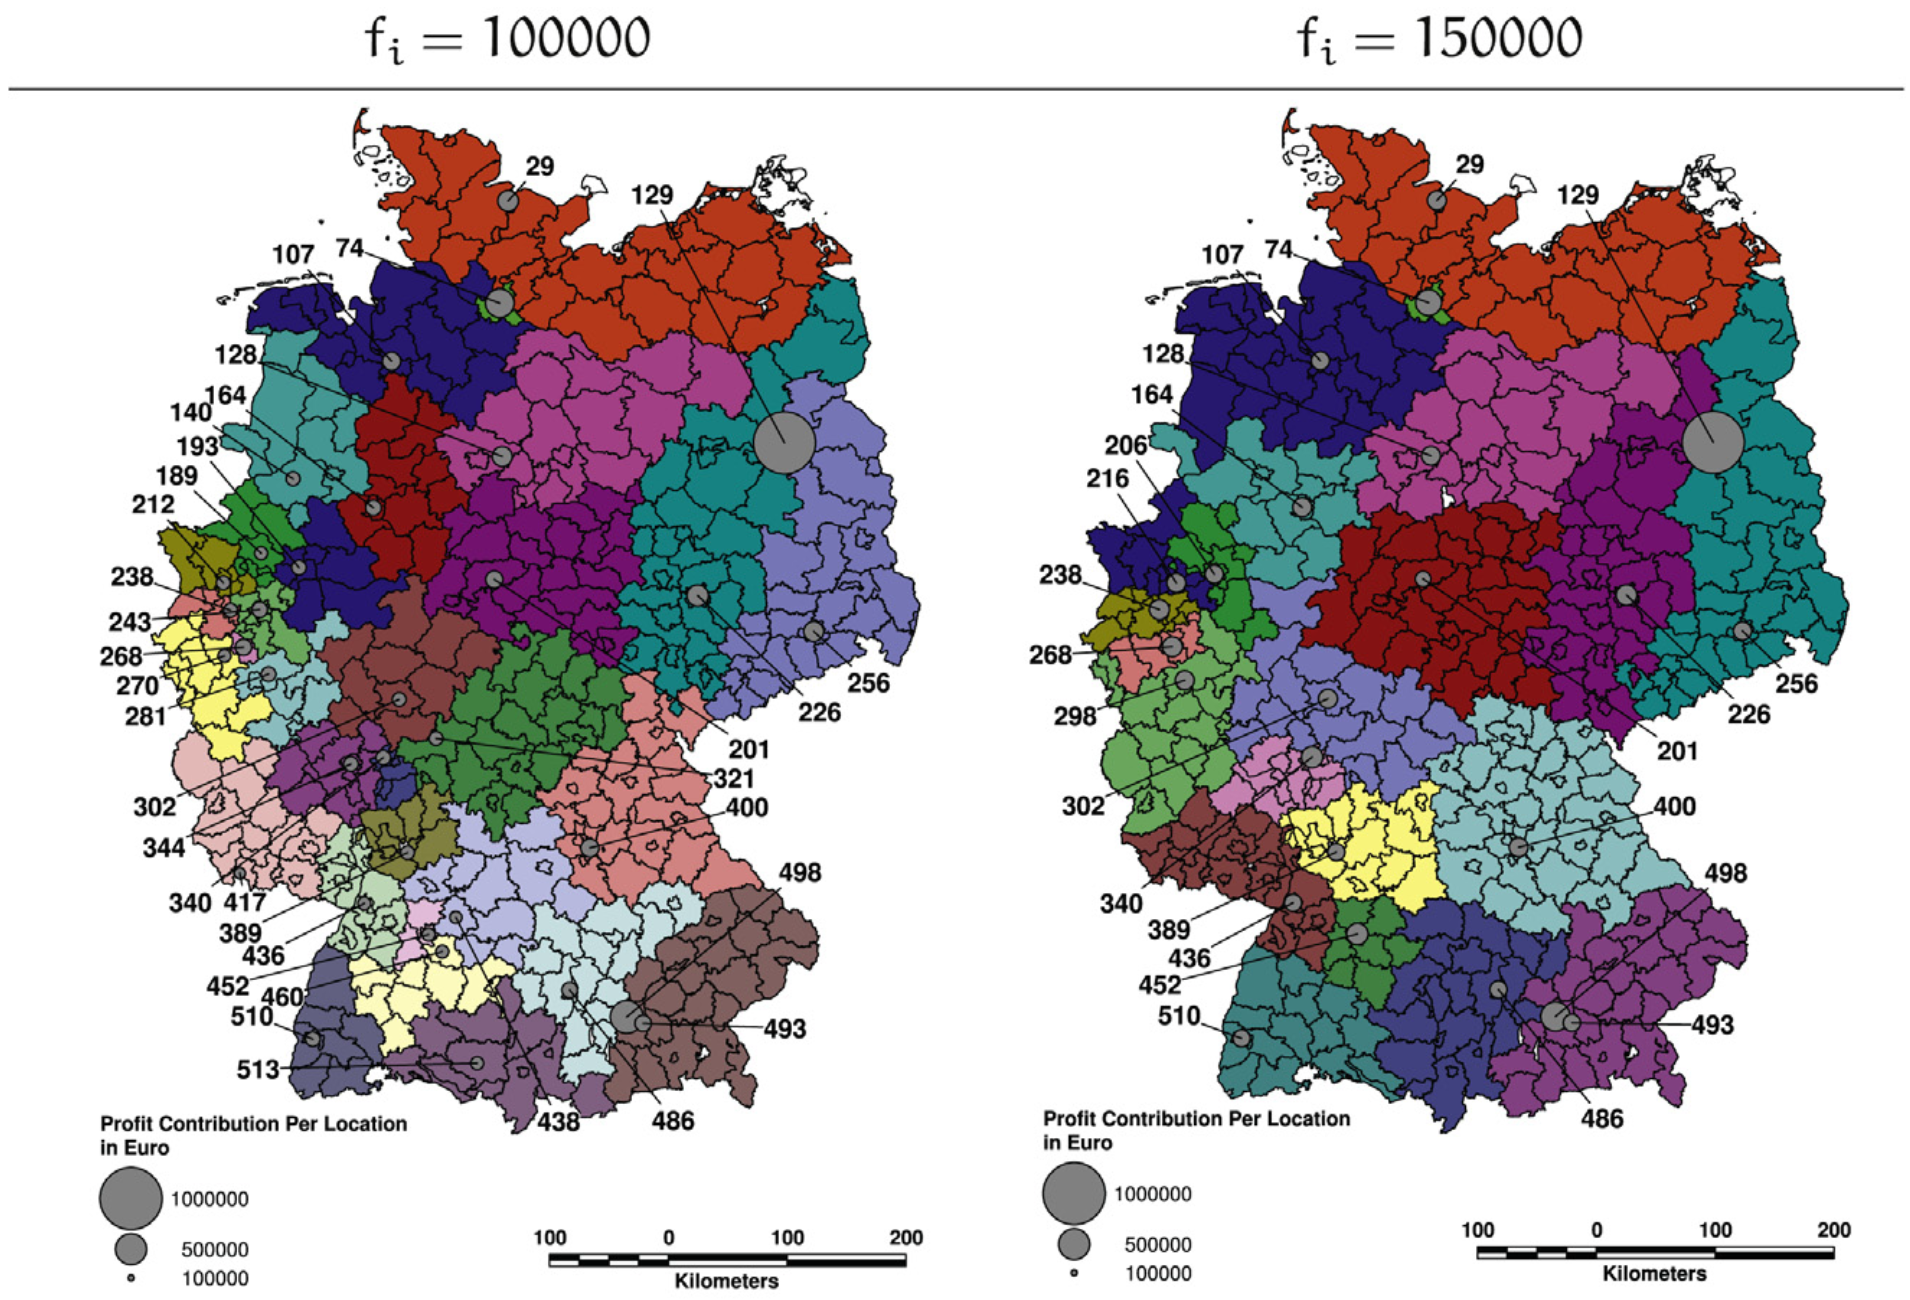
\includegraphics[width=.75\textwidth]{map1.png}
\end{frame}

\begin{frame}{\textbf{Case study: Pharmaceutical industry}}
\centering 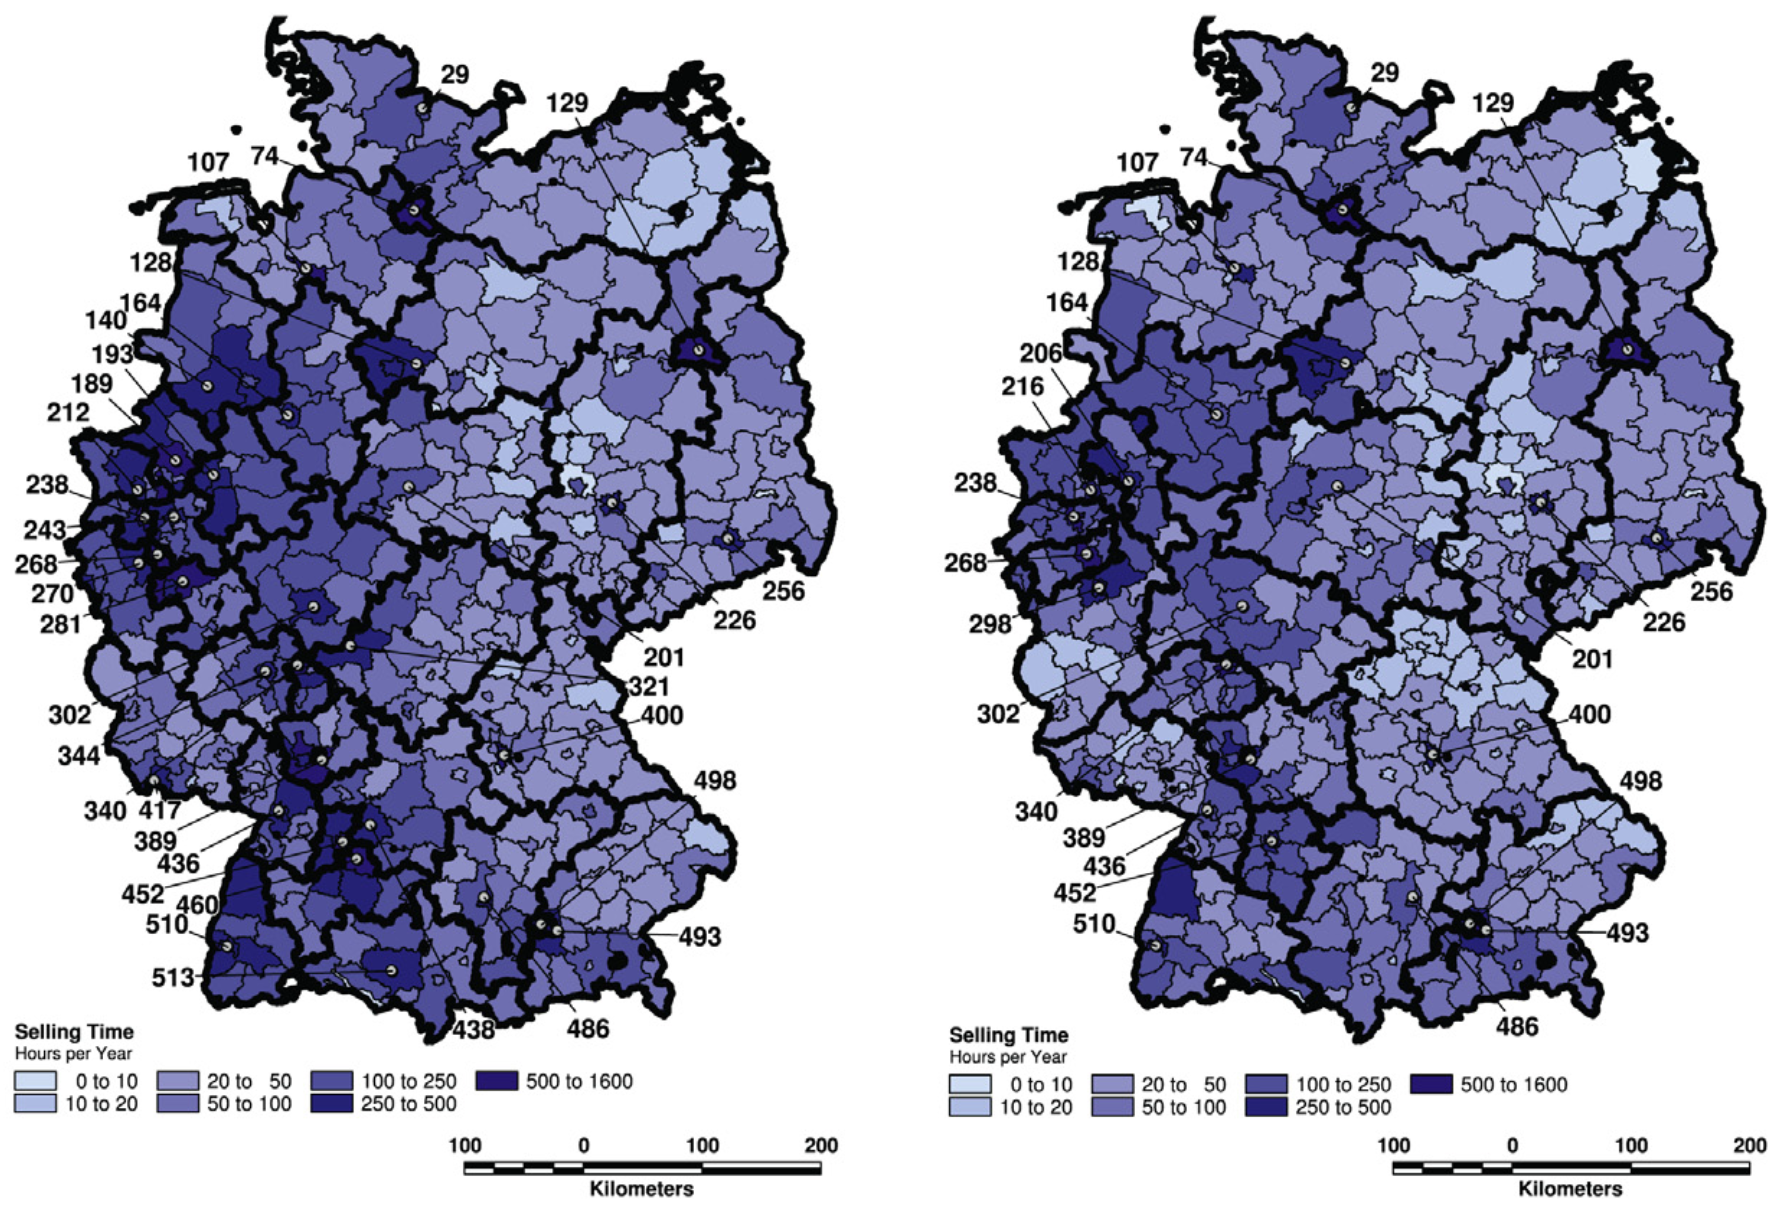
\includegraphics[width=.75\textwidth]{map2.png}
\end{frame}

\begin{frame}{\textbf{Case study: Pharmaceutical industry}}
\centering 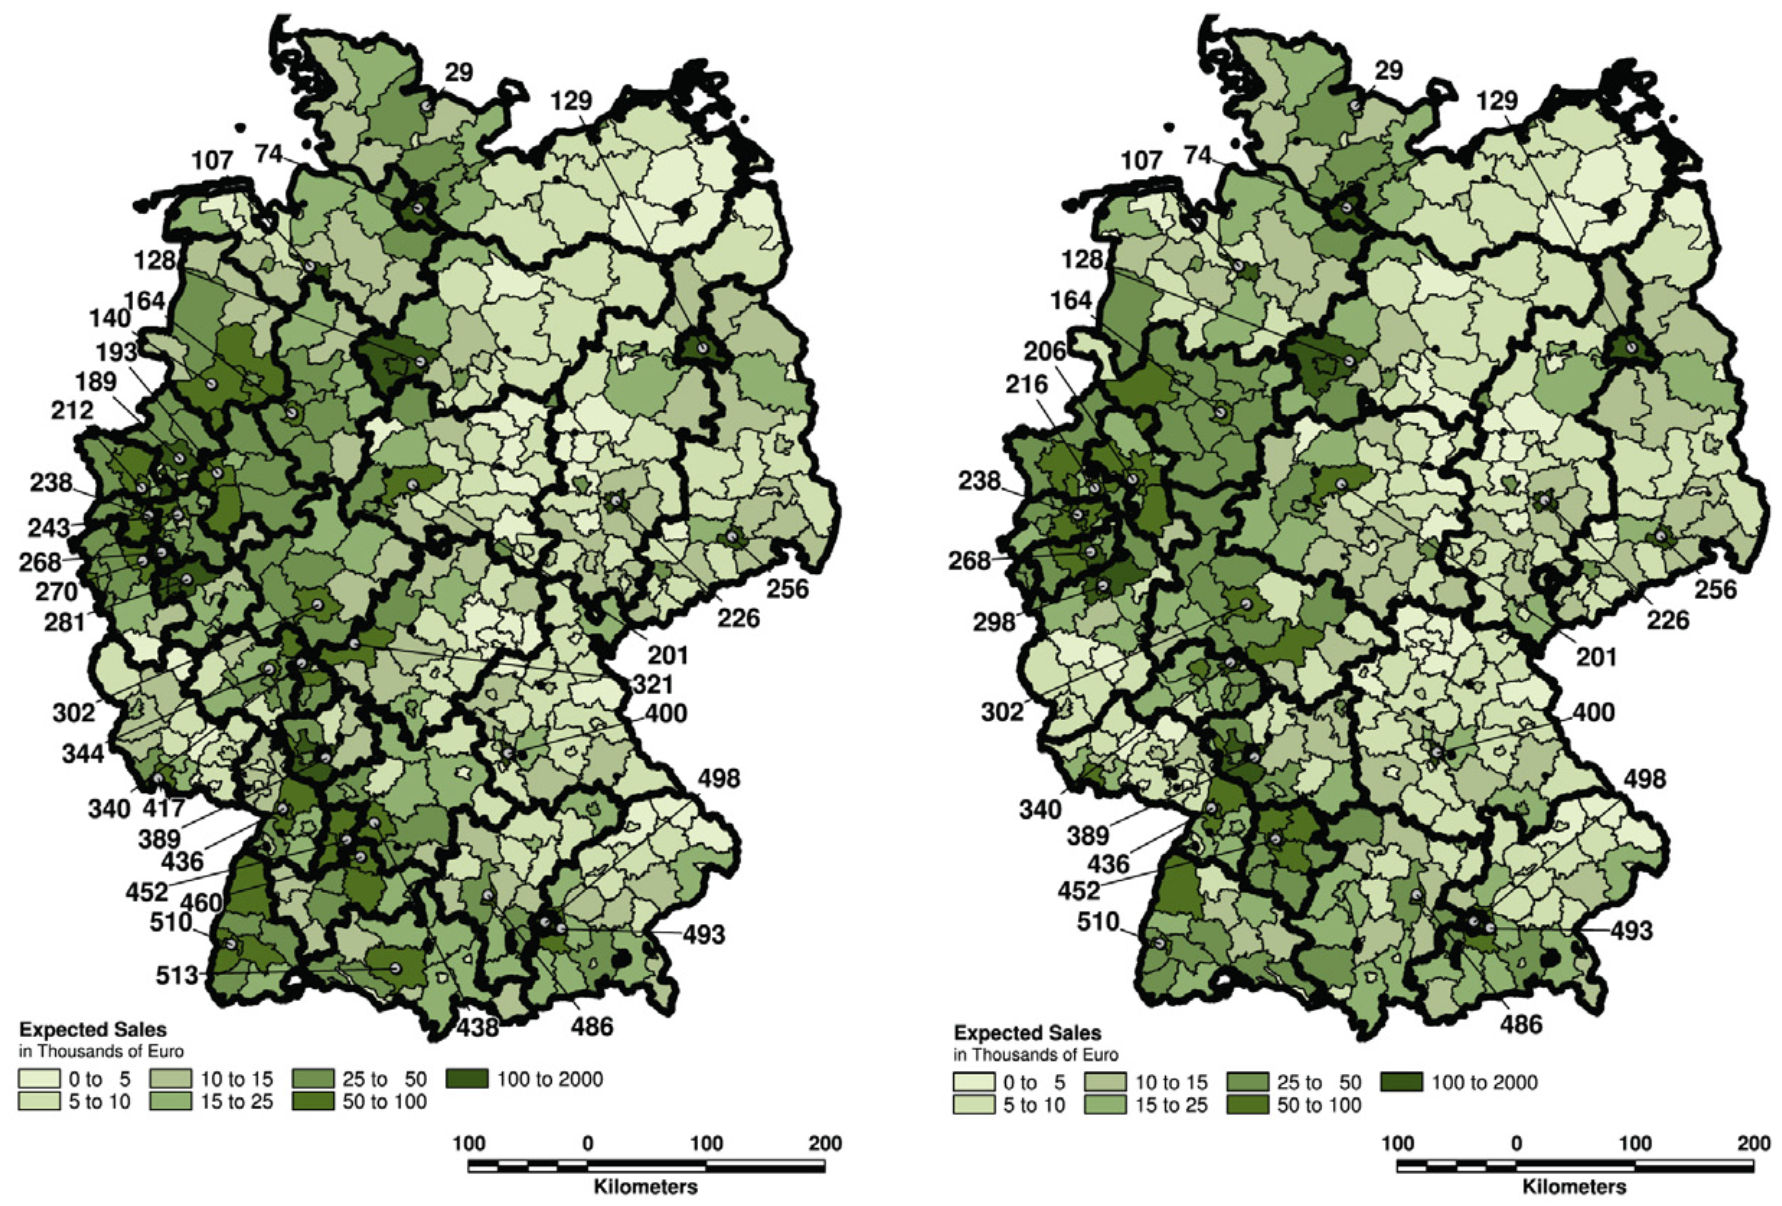
\includegraphics[width=.75\textwidth]{map3.png}
\end{frame}

\begin{frame}
  \centering
 \Large  \textbf{One more thing!}
\end{frame}

\begin{frame}{\textbf{Profit vs. Fairness}}
\centering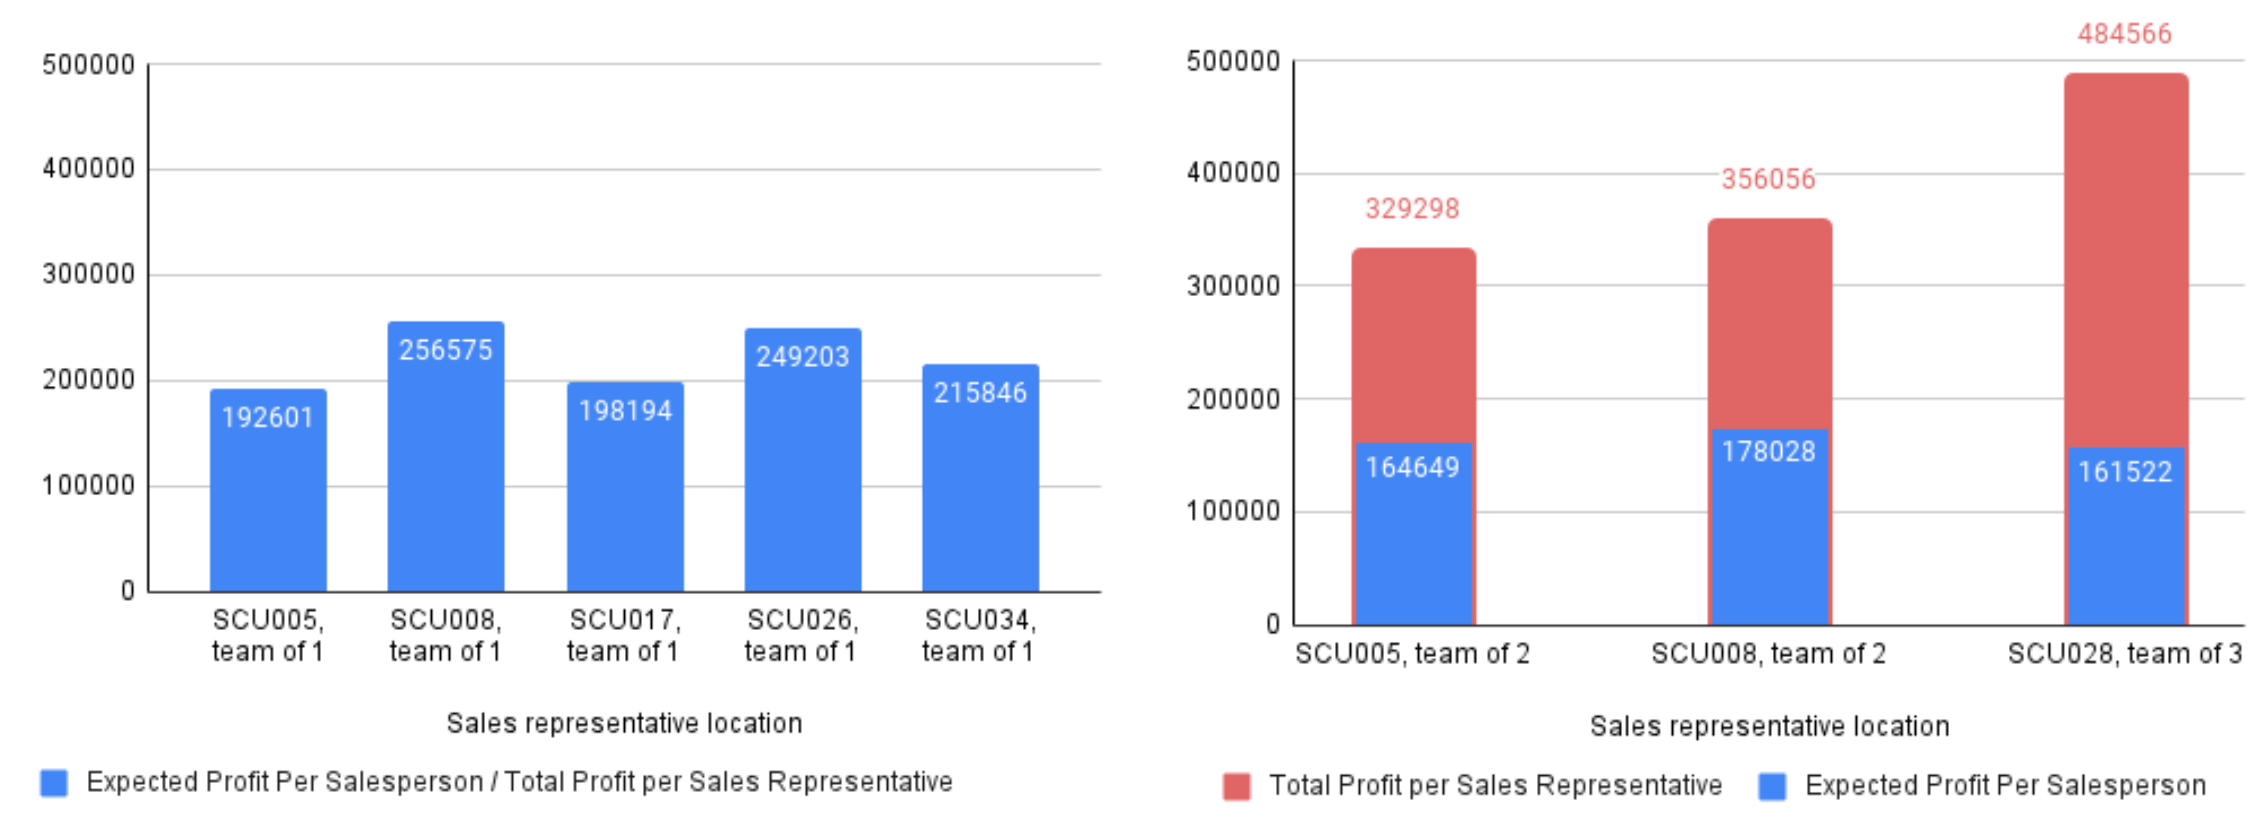
\includegraphics[width=0.95\textwidth]{singleVsmulti.png}
\end{frame}


\begin{frame}{\textbf{Profit vs. Fairness}}
\centering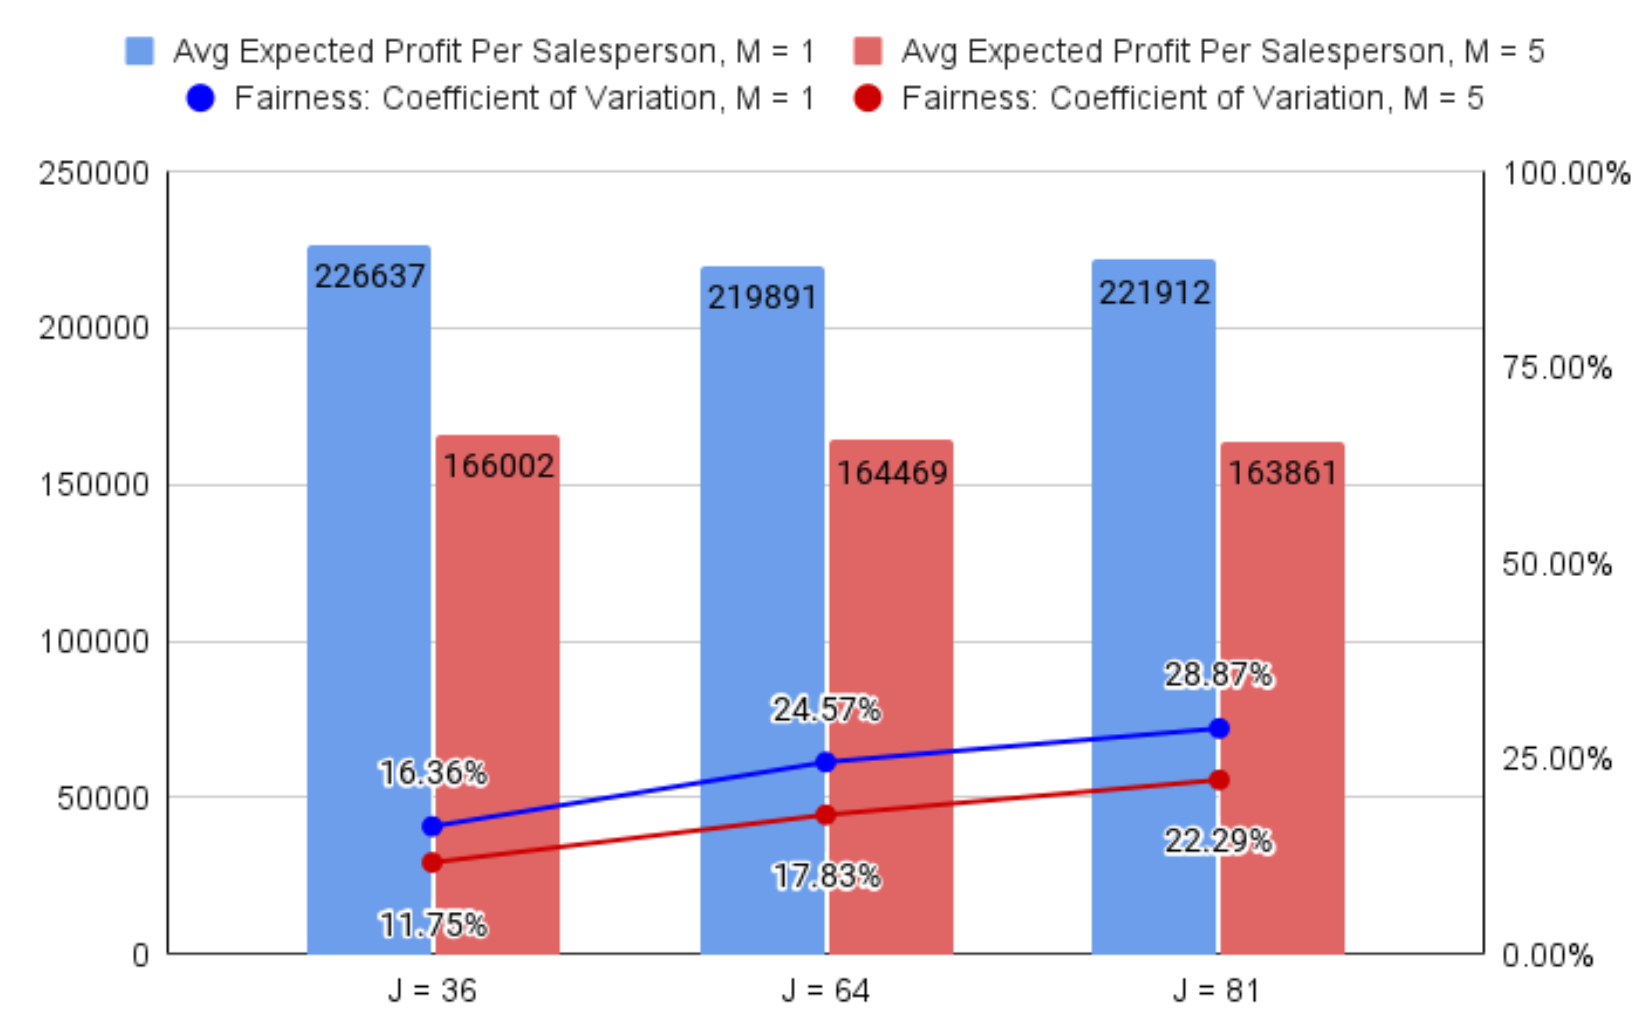
\includegraphics[width=0.8\textwidth]{fairness_1.png}
\end{frame}

\begin{frame}{\textbf{Profit vs. Fairness}}
\centering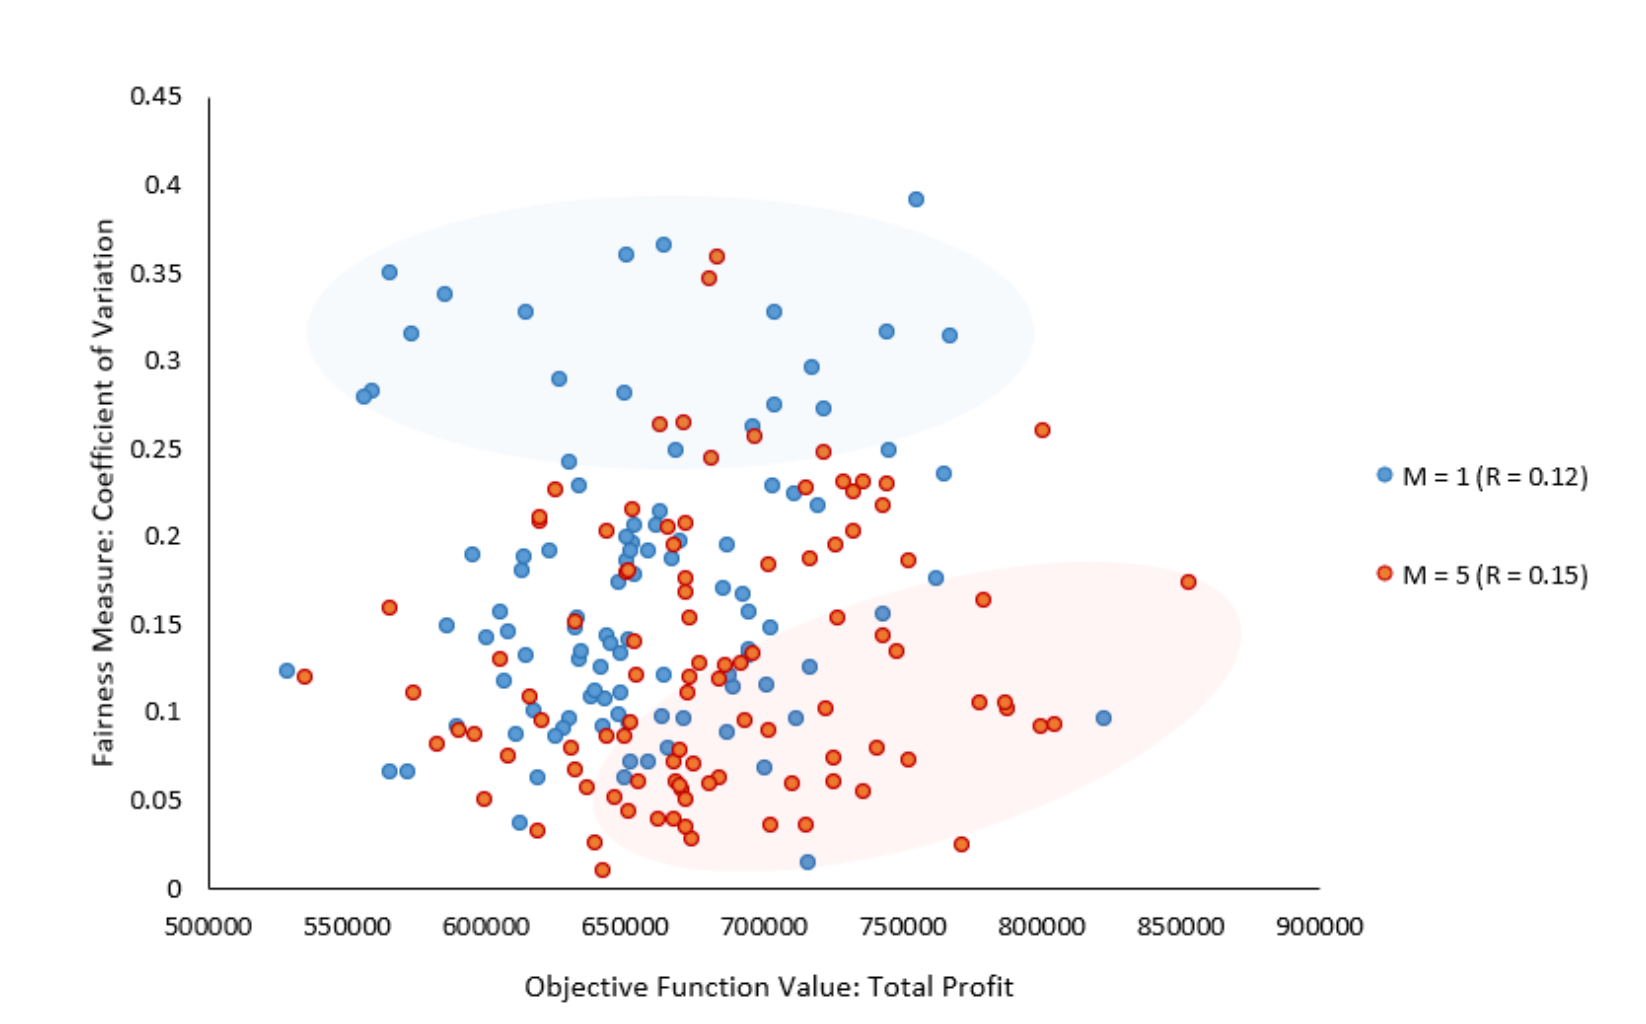
\includegraphics[width=0.85\textwidth]{fairness_2.png}
\end{frame}

\begin{frame}{\textbf{Profit vs. Fairness}}
\centering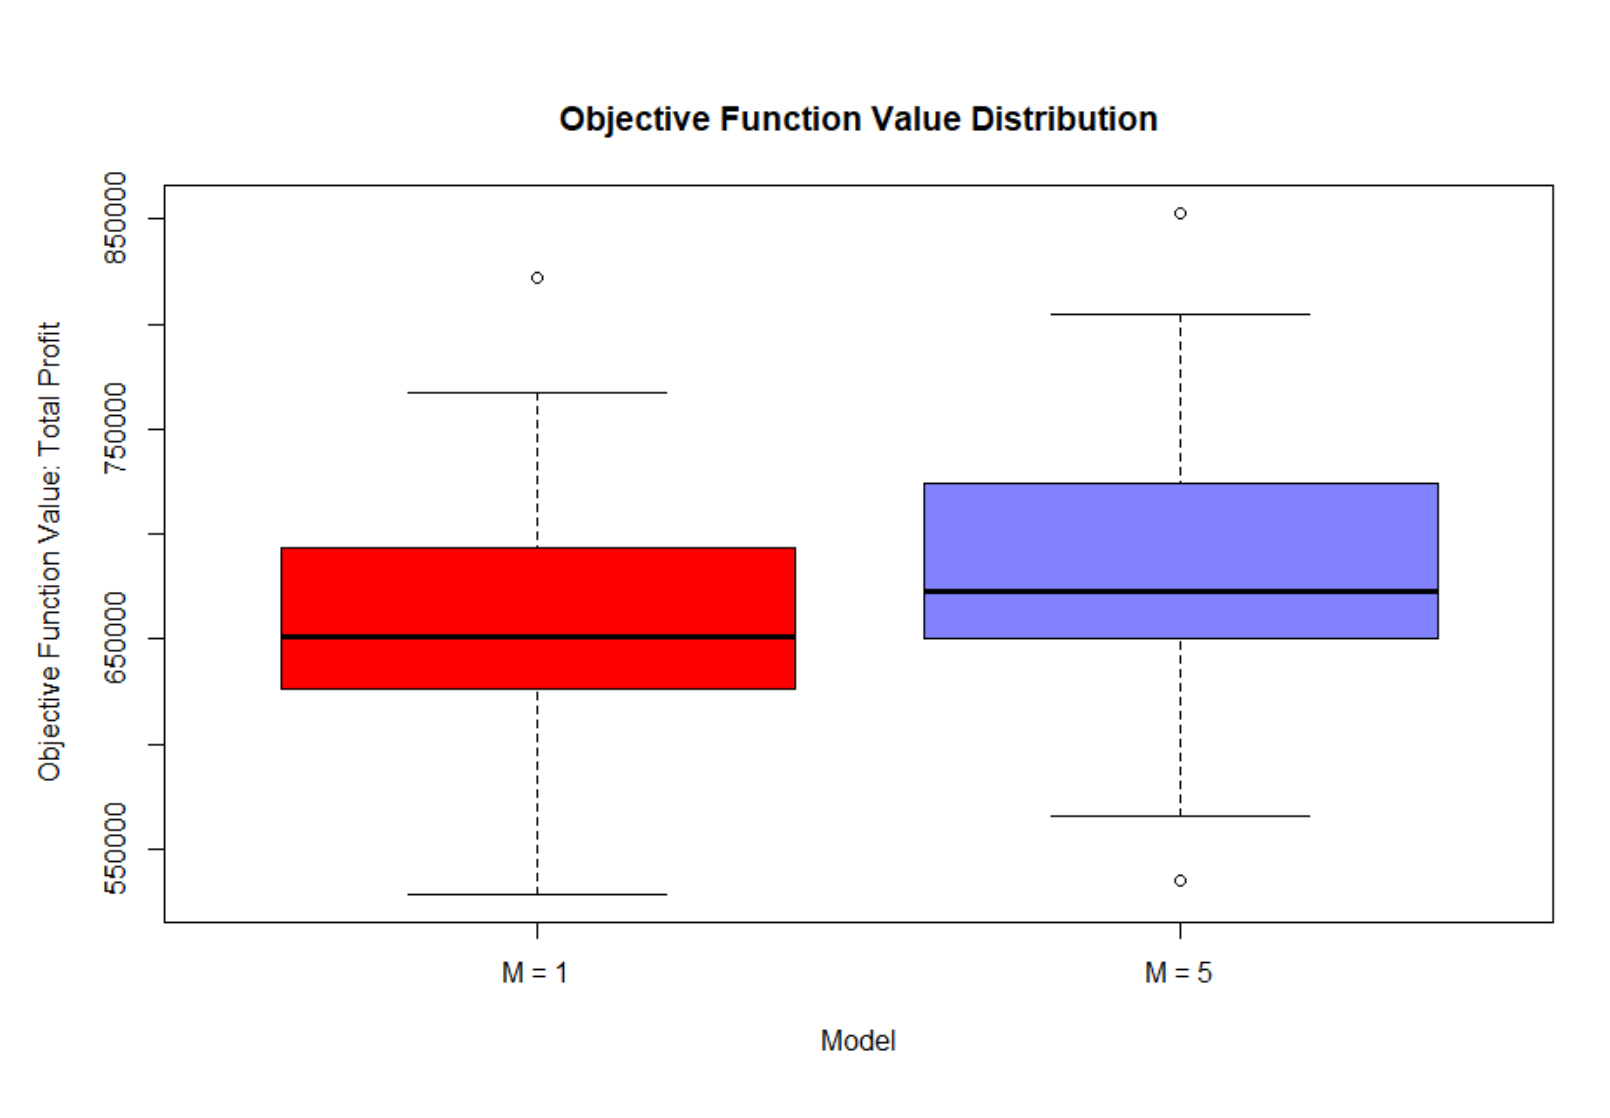
\includegraphics[width=0.45\textwidth]{obj.png}
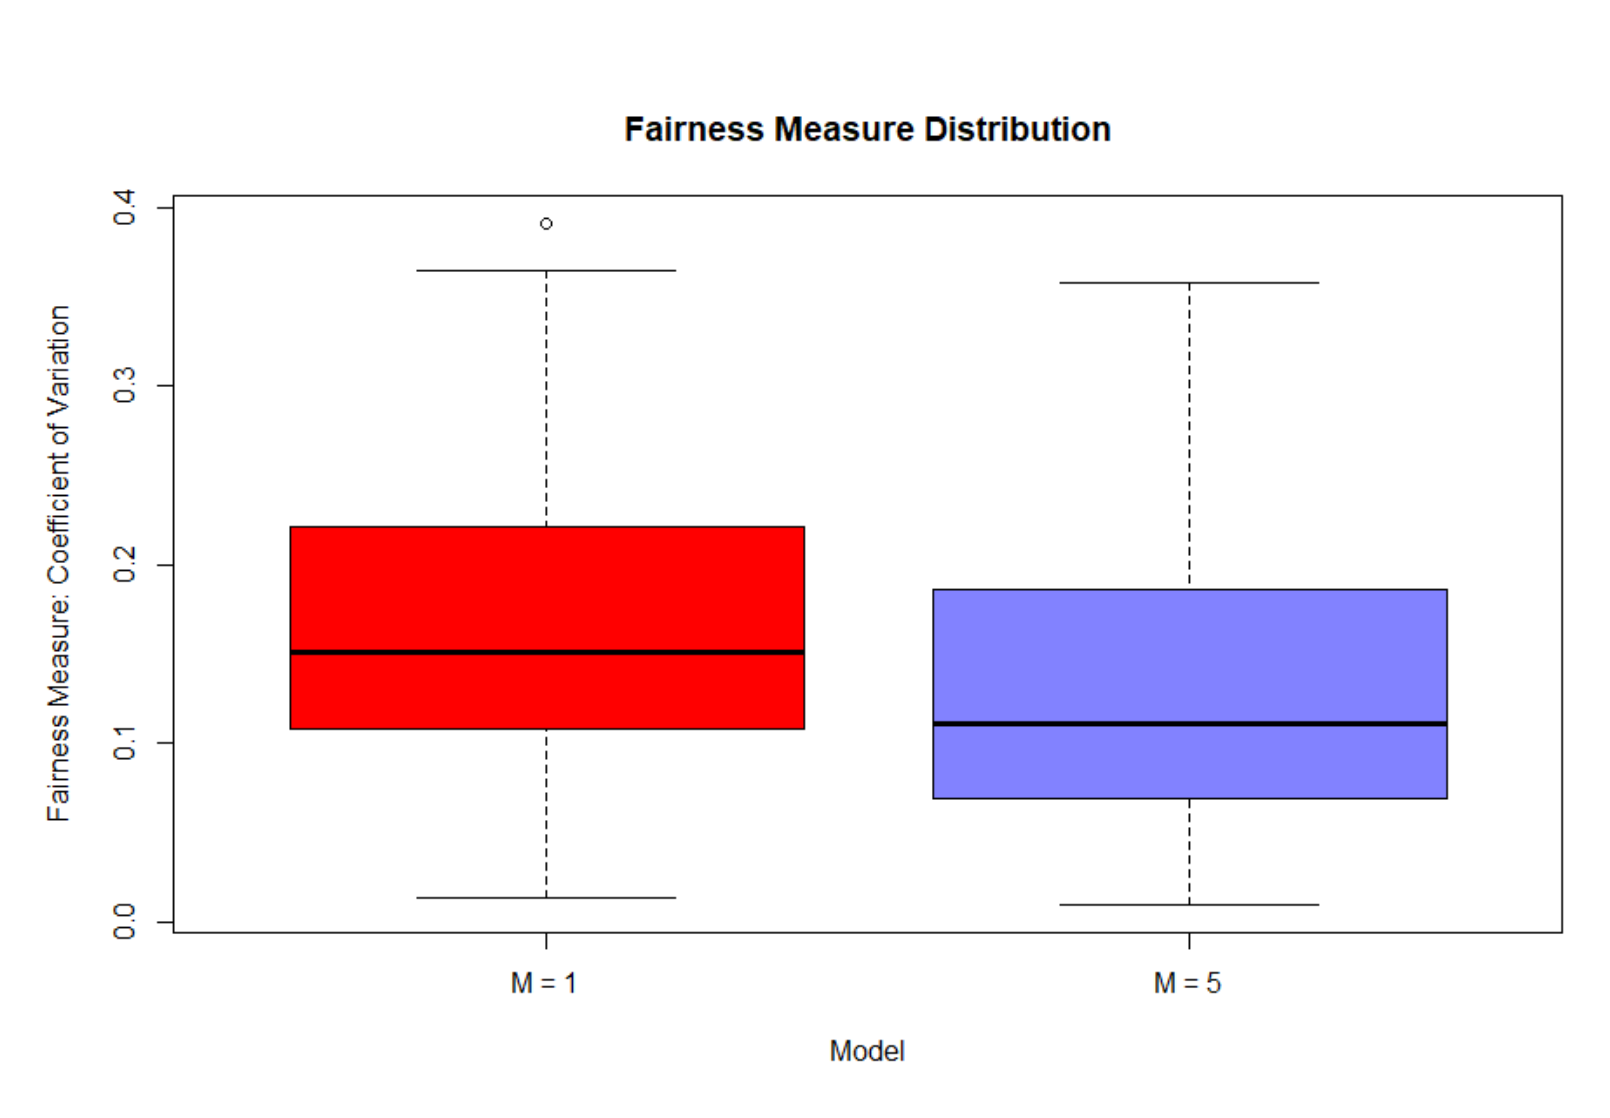
\includegraphics[width=0.45\textwidth]{fair.png}
\end{frame}

\begin{frame}
  \centering
 \Large  \textbf{Be fair and profitable}
\end{frame}

\end{document}

